\documentclass[twoside,12pt]{book}

\usepackage{gensymb}
\usepackage[resetlabels]{multibib}
\usepackage[T1]{fontenc}
\usepackage{graphicx}
\usepackage{multirow}
\usepackage{amsmath}
\usepackage{amssymb}
\usepackage{appendix}                % provides subappendices
\usepackage{etoolbox}                % to add sub appendices to toc
\AtBeginEnvironment{subappendices}{
\addcontentsline{toc}{chapter}{Appendices}
\counterwithin{figure}{section}
\counterwithin{table}{section}
\counterwithin{equation}{section}
}
\usepackage[capitalize]{cleveref}                % simplify references to Eqs., Figs., Tabs.
%\usepackage{natbib}
\newcommand{\ifprivate}{\iftrue}     % activate this line for a private version
%\newcommand{\ifprivate}{\iffalse}    % activate this line for a public version

\input{manualstyle}
%
\sloppy\raggedbottom
\pagestyle{headings}
\graphicspath{ {./figs/} {../../tools/nuclear_scattering/figs/} }
                % to add other graphics paths, just add other {./...} items
\usepackage[font={small}]{caption}

\newcommand{\mathAA}{\mathring{\mathrm{A}}}
\renewcommand{\eqref}[1]{Eq.~(\ref{#1})}
%
\begin{document}
%
\bibliographystyle{unsrt}
%
%%%%%%%%%%%%%
% Titlepage %       Remark: for printing the titlepage font cmr17 scaled
%%%%%%%%%%%%%               \magstep7 is required.
%
\begin{titlepage}
\newfont{\titlefont}{cmr17 scaled\magstep5}
\newfont{\authorfont}{cmbx12 scaled\magstep2}
%
\begin{center}
{
\vspace*{4cm}
%
\titlefont
Nuclear Scattering \\[1ex]
Theoretical Background \\[3cm]
%
\authorfont
G. Hobler \\[3cm]
}
%
Institute of Solid-State Electronics,
TU Wien, AUSTRIA \\[1ex]

%December 2009 \\ \vspace*{4cm}
%
\today
%
\end{center}

\end{titlepage}
%
%%%%%%%%%%%%%%%%%%%%%%
% Inhaltsverzeichnis %
%%%%%%%%%%%%%%%%%%%%%%
%
\tableofcontents
\thispagestyle{empty}
%
%%%%%%%%%%%%%%%%%%%%
% Nuclear Stopping %
%%%%%%%%%%%%%%%%%%%%
%
\chapter{Nuclear Stopping}
\label{k:sn}
%
\section{Binary Collision Physics}
\label{s:bcp}
% Binary Collision Physics

In the binary collision approximation (BCA), the interaction of an energetic atom (``ion'' or ``projectile'', index 1) with a target atom (``recoil'', index 2) is treated as a sequence of isolated events, the binary collisions.
In each collision, the trajectories are approximated by their asymptotes.
Incoming and outgoing asymptote are the straight lines that are fitted to the trajectories long enough before and after the collision, respectively, assuming that there is no interaction with any other target atom.
They are indicated in \cref{fig:sn_trajectories} by dashed lines.
%
\begin{figure}[htbp]
    \centering
    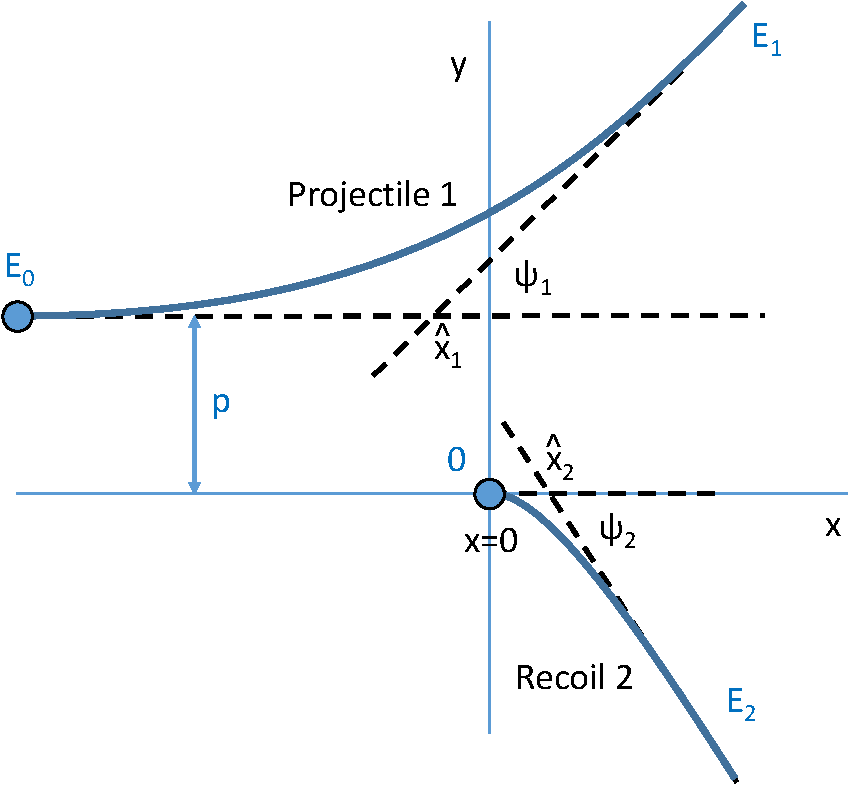
\includegraphics[scale=0.6]{trajectories.pdf}
    \caption{Ion and recoil trajectory and their asymptotes.
        The initial ion energy is $E$; $T_\mathrm{n}$ is transfered from the ion to the recoil during the collision.
        The energy transfer $T_\mathrm{n}$ and the scattering angles $\psi$ and  $\psi_\mathrm{R}$ depend on the initial ion energy $E$ and the impact parameter $p$.
        The origin of the coordinate system is chosen in the intial recoil position, and the $x$ axis is parallel to the direction of the incoming ion.
        \label{fig:sn_trajectories}
    }
\end{figure}
%
The outgoing trajectories are characterized by the scattering angle of the ion, $\psi$, the recoil angle $\psi_\mathrm{R}$, and the intersection points of the asymptotes, which are given by $(x_1,p)$ and $(x_2,0)$ in the coordinate system of \cref{fig:sn_trajectories}.
These characteristics depend on the ion energy $E$ before the collision, the impact parameter $p$ (the distance of the target atom before the collision from the incoming ion asymptote), and the interatomic potential $V(r)$ which is assumed to depend on the internuclear distance only.
The interatomic potential depends on the properties of the projectile and the recoil, i.e., the masses $M_1$ and $M_2$ and atomic numbers $Z_1$ and $Z_2$.
During the collision, the ion transfers energy $T_\mathrm{n}$ to the recoil, so the ion energy after the collision is $E - T_\mathrm{n}$, and the recoil energy is $T_\mathrm{n}$, if we assume the collision to be elastic and the recoil is at rest before the collision.

In this section we present the results of the classical theory of scattering for the scattering angles $\psi$ and $\psi_\mathrm{R}$, for the energy transfer $T_\mathrm{n}$, and for the coordinates $x_1$ and $x_2$ of the intersection points of the trajectory asymptotes, compare \cref{fig:sn_trajectories}.
Derivations can be found in Ref.~\cite{Eck91}.

In the classical theory of scattering \cite{Bohr1948,ZBL85} the scattering angles $\psi$ and $\psi_\mathrm{R}$ and the energy transfer $T_\mathrm{n}$ are expressed in terms of the scattering angle $\theta$ in the center-of-mass (CM) system
%
\begin{equation}
    \label{eq:sn_physics_psi}
    \tan \psi = \frac{ \sin\theta }{ \cos\theta + \frac{M_1}{M_2} }, \quad
    \psi_\mathrm{R} = \frac{\pi - \theta}{2} ~,
\end{equation}
%
\begin{equation}\label{eq:sn_physics_dE}
    T_\mathrm{n} = \frac{ 4 M_1 M_2 }{ (M_1 + M_2)^2 } \, E \,
        \sin^2 \frac{\theta}{2} ~.
\end{equation}
%
$\theta$ is given by \cite{Lan90}%
%
\footnote{We do not write $\theta$ explicitly because for very small $\theta$ this would result in a loss of accuracy in cases where actually $\pi - \theta$ is needed, if $\theta$ were first calculated by the difference of $\pi$ and the integral, and then $\pi - \theta$ were calculated as the difference between $\pi$ and $\theta$. Note that $\sin \frac{\theta}{2} = \cos \frac{\pi - \theta}{2}$, $\cos \frac{\theta}{2} = \sin \frac{\pi - \theta}{2}$.}
%
\begin{equation}
    \label{eq:sn_physics_theta}
    \pi - \theta = 2 \, p \int_{r_0}^\infty
        \frac{ \mathrm{d}r }{
            r^2 \sqrt{ 1 - \frac{ V(r) }{ E_\mathrm{c} } - \frac{ p^2 }{ r^2 } } } ~.
\end{equation}
%
$r_0$ denotes the distance of closest approach between the ion and the recoil, which is given by the root of the expression under the square root, i.e.,
%
\begin{equation}
    \label{eq:sn_physics_r0}
    1 - \frac{ V(r_0) }{ E_\mathrm{c} } - \frac{ p^2 }{ r_0^2 } = 0
\end{equation}
%
The numerical solution of \cref{eq:sn_physics_r0} is discussed in Section~\ref{s:apsis}.
$E_\mathrm{c}$ denotes the energy in the center-of-mass system
%
\begin{equation}
    \label{eq:sn_physics_Ec}
    E_\mathrm{c} = \frac{ M_2 }{ M_1 + M_2 } \, E .
\end{equation}
%
The coordinates of the intersection points of the trajectory asymptotes may be expressed in terms of $\theta$ and the so-called time integral $\tau$. In the coordinate system of \cref{fig:sn_trajectories} these points are at $(\hat{x}_1,p)$ and $(\hat{x}_2,0)$ with%
%
\footnote{
    More sophisticated formulae that take electronic energy loss in the middle of the collision into account are presented in Ref.~\cite{Eck91}.
    They may be used in IMSIL if desired, but the added accuracy is deemed marginal.
}
%
\begin{equation}
    \label{eq:sn_recoil_turning}
    \hat{x}_2 = \frac{ 2 M_1 }{ M_1 + M_2 } \, (p \, \tan \frac{\theta}{2} - \tau)
\end{equation}
%
and
%
\begin{equation}
    \label{eq:sn_proj_turning}
    \hat{x}_1 = \hat{x}_2 - p \, \tan \frac{\theta}{2}.
\end{equation}
%
The time integral $\tau$ is given by \cite{Rob97}%
%
\footnote{
    A different formula is used in Ref.~\cite{Eck91}. We prefer \cref{eq:sn_tau}, since it is somewhat simpler to evaluate, and it can also be used for attractive interatomic potentials.
}
%
\begin{equation}
    \label{eq:sn_tau}
    \tau = r_0 - \int_{r_0}^\infty \left[
        \frac{ 1 }{ \sqrt{ 1 - \frac{ V(r) }{ E_\mathrm{c} }
                - \frac{ p^2 }{ r^2 } } }
        - 1 \right] \mathrm{d}r.
\end{equation}
%
Note, in spite of its name, the time integral $\tau$ has units of a length.



%
\section{Scattering Quantities for Screened Coulomb Potentials}
\label{s:screen}
% Scattering Quantities for Screened Coulomb Potentials

\subsection{Screened Coulomb Potentials}
%%%%%%%%%%%%%%%%%%%%%%%%%%%%%%%%%%%%%%%%
%
For small internuclear distances $r$, the interaction between two atoms is described by the Coulomb potential.
It is therefore common to write the interatomic potential as a screened Coulomb potential
%
\begin{equation}
    \label{eq:sn_screened_coulomb}
    V(r) = \frac{Z_1 Z_2 e^2}{r} \, \Phi\left( \frac{r}{a_\mathrm{I}} \right)
\end{equation}
%
where the screening function $\Phi$ describes the deviation from the Coulomb potential and $\Phi(r \rightarrow 0) = 1$.
The Coulomb potential is given by
%
\begin{equation}
    \label{eq:sn_coulomb}
    V_\mathrm{Coul} = \frac{1}{4 \pi \varepsilon_0} \frac{Z_1 Z_2 e^2}{r} \approx
        14.3996439 \, \mathrm{eV} \, \frac{Z_1 Z_2}{r[\mathrm{\mathAA}]} \approx
        14.4 \, \frac{Z_1 Z_2}{r[\mathrm{\mathAA}]} \, \mathrm{eV} ~.
\end{equation}
%
The argument of $\Phi$ is usually scaled by a screening length $a_I$, which is chosen as to make $\Phi(r/a_\mathrm{I})$ approximately independent of the atom species.
The most common choices of $a_\mathrm{I}$ are according to Firsov \cite{Fir58}
%
\begin{equation}
    \label{eq:sn_aF}
    a_\mathrm{F} = \frac{ 0.46850 \mathAA }{ \left( Z_1^{1/2} + Z_2^{1/2} \right) ^ {2/3} } ~,
\end{equation}
%
Lindhard \cite{Lin68}
%
\begin{equation}
    \label{eq:sn_aL}
    a_\mathrm{L} = \frac{ 0.46850 \mathAA }{ \left( Z_1^{2/3} + Z_2^{2/3} \right) ^ {1/2} } ~,
\end{equation}
%
and ZBL \cite{ZBL85}
%
\begin{equation}
    \label{eq:sn_aZBL}
    a_\mathrm{ZBL} = \frac{ 0.46850 \mathAA }{ Z_1^{0.23} + Z_2^{0.23} } ~.
\end{equation}

For the screening function $\Phi$, a sum of exponentials
%
\begin{equation}
    \label{eq:sn_sum_exp}
    \Phi(R) = \sum_{i=1}^n a_i \exp(-b_i R)
\end{equation}
%
is often used, where \(a_i\) and \(b_i\) are coefficients.
The requirement \(\Phi(0) = 1\) results in \(\sum_i a_i = 1\).
The values of the coefficients for common potentials potential are listed in \cref{tab:sn_screen_coefs}.
The Moliere \cite{Bie80} and KrC \cite{Wil77} screening function are meant to be used with the Firsov screening length, while the ZBL scrrening function \cite{ZBL85} is used with the ZBL screening length.
%
\begin{table}
    \caption{Coefficients of the sum or exponentials, \cref{eq:sn_sum_exp}, for the Moliere \cite{Mol47}, KrC \cite{Wil77}, and ZBL potential \cite{ZBL85}.}
    \label{tab:sn_screen_coefs}
    \centering
    \begin{tabular}{|cc|cc|cc|}
        \hline
        \multicolumn{2}{|c|}{Moliere} & \multicolumn{2}{c|}{KrC} & \multicolumn{2}{c|}{ZBL} \\
        $a_i$ & $b_i$ & $a_i$    & $b_i$    & $a_i$   & $b_i$ \\
        \hline
        0.1   &  6    & 0.335381 & 1.919249 & 0.18175 & 3.1998 \\
        0.55  & 1.2   & 0.473674 & 0.637174 & 0.50986 & 0.94229 \\
        0.35  & 0.3   & 0.190945 & 0.278544 & 0.28022 & 0.4029 \\
              &       &          &          & 0.02817 & 0.20162 \\
        \hline
    \end{tabular}
\end{table}

Atom-pair specific interatomic potentials have also been proposed:
The coefficients for pair-specific ZBL interatomic potentials are contained in the POTCOEF03.DAT file of the Data folder of SRIM-2013 \cite{SRIM-2013}.%
%
\footnote{According to the version history that comes up when pushing the “SRIM-2013.00” button in the SRIM-2013 Main Window, the pair-specific potentials seem to have been introduced in SRIM-2003.00. They are most likely not used by the Monte Carlo TRIM code of SRIM.
}
%
More recently, pair-specific NLH potentials \cite{Nor25} have been proposed, which are fits to all-electron density functional theory (DFT) calculations.%
%
\footnote{The NLH potentials are not meant to be used for binary collision approximation simulations as they have not been fitted to the low-energy parts of the interatomic potential.
}
%

The sum-of-exponentials screening function, \cref{eq:sn_sum_exp}, has infinite range.
In reality, the interatomic potential goes to zero at some internuclear distance $r_\mathrm{max}$, and is negative for $r > r_\mathrm{max}$, resulting in an attractive part of the potential.
The DFT data can be well fitted by a combination of a sum-of-exponentials and a linear function up to $r = r_\mathrm{max}$ \cite{Hob24}
%
\begin{equation}
    \label{eq:sn_NLHlin}
    \Phi(R) = \sum_{i=1}^n a_i \left[ \exp(-b_i R) - \exp(-b_i R_\mathrm{max}) \right]
        - d \left( 1 - \frac{ R }{ R_\mathrm{max} } \right) ~,
\end{equation}
%
where $R_\mathrm{max} = r_\mathrm{max} / a_\mathrm{I}$.
A simple choice for $r > r_\mathrm{max}$ is $\Phi(R) = 0$, resulting in a finite-range interatomic potential.
An advantage of finite-range interaction from a computational point of view is that there is a clear criterion for what atoms the ion interacts with as it travels in the target.
Because of the linear term in \cref{eq:sn_NLHlin} we call the potential with this screening function the NLHlin potential.

\begin{figure}
    \centering
    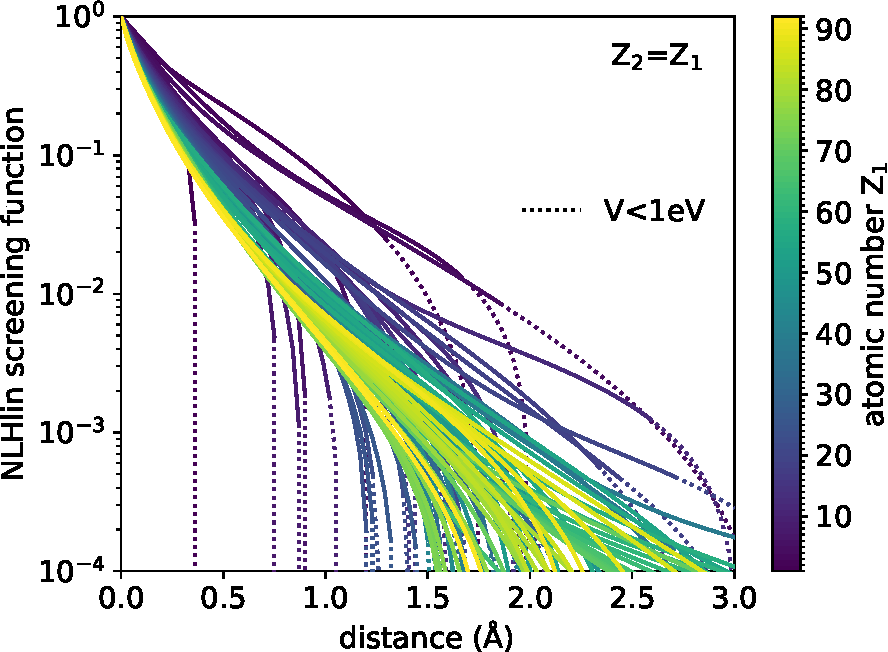
\includegraphics[scale=0.5]{nlhlin_unscaled.pdf} ~~
    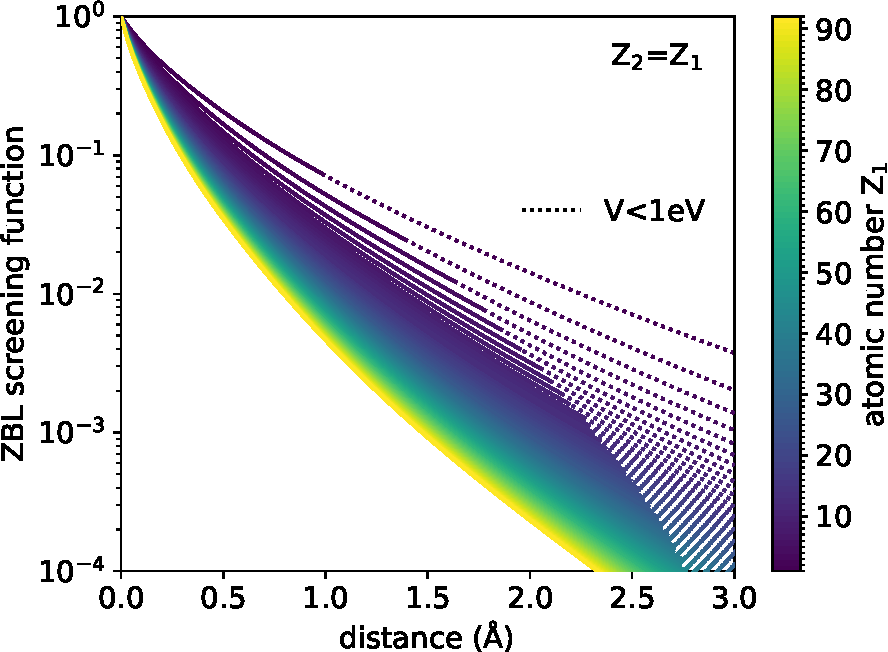
\includegraphics[scale=0.5]{zbl_unscaled.pdf}
    \caption{NLHlin (left) and ZBL (right) screening function for homonuclear atom pairs ($Z1=Z_2$) as a function of internuclear distance in {\AA}ngst{\o}ms.}
    \label{fig:sn_screen}
\end{figure}
%
In \cref{fig:sn_screen} the NLHlin and the ZBL potential are shown for homonuclear atom pairs ($Z1=Z_2$) as a function of the unscaled internuclear distance $r$. The ZBL screening function expectedly does not describe the drop-off towards the maximum range and overestimates the tails at least for some of the lighter elements.

\begin{figure}
    \centering
    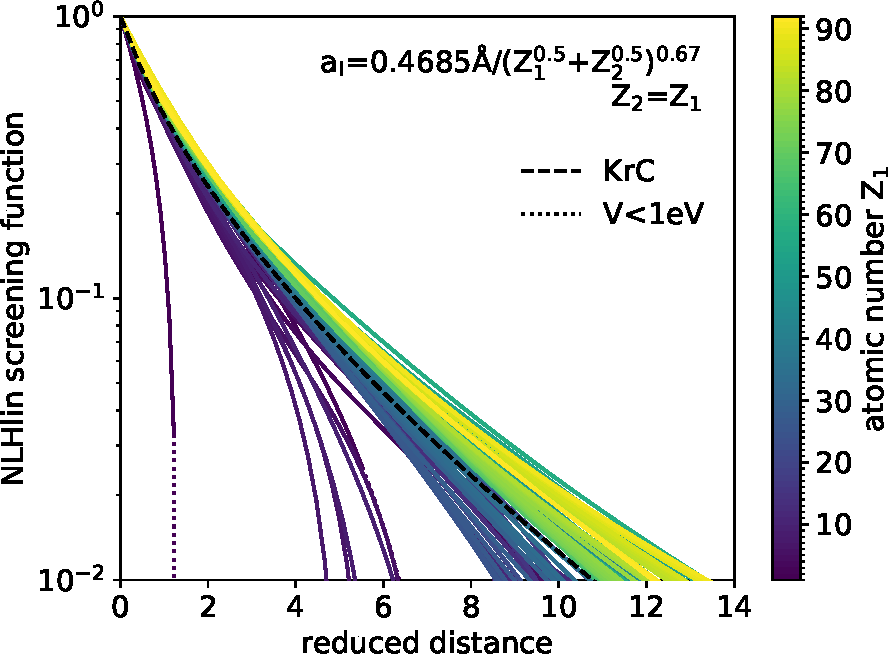
\includegraphics[scale=0.5]{nlhlin_p0.5_p0.67.pdf} ~~
    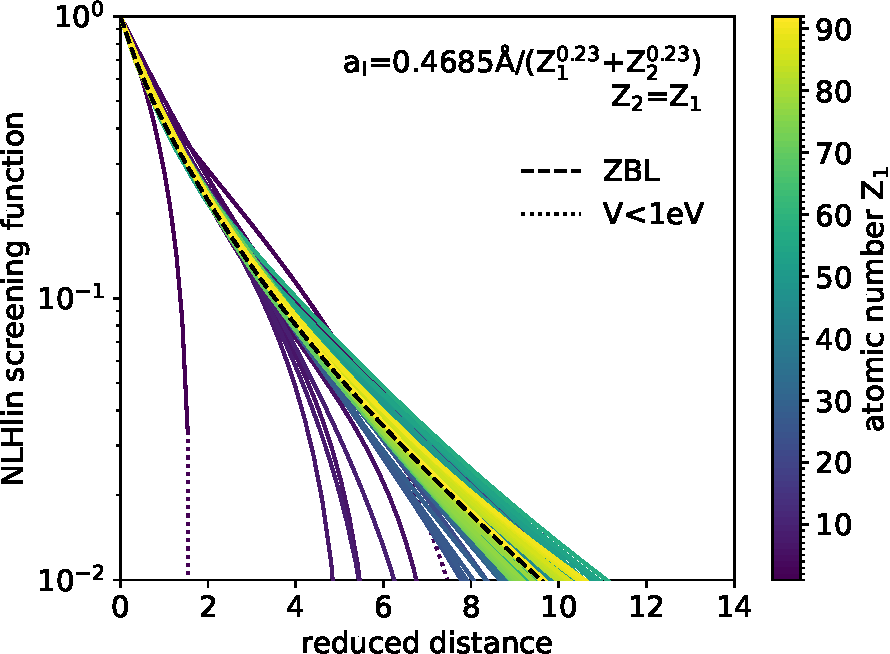
\includegraphics[scale=0.5]{nlhlin_p0.23_p1.pdf}
    \caption{NLHlin screening function for homonuclear atom pairs ($Z_1=Z_2$) as a function of internuclear distance scaled with the Firsov screening length \cref{eq:sn_aF} (left) and the ZBL  screening length \cref{eq:sn_aZBL} (right).}
    \label{fig:sn_screen_scaled}
\end{figure}
%
It is interesting to attempt finding a screening length that compresses the screening function to a single function. Simple formulae such as \crefrange{eq:sn_aF}{eq:sn_aZBL} cannot be expected to describe the range $r_\mathrm{max}$ of the potentials because it mainly depends on the number of valence electrons of the elements. However, one can try to compress the screening functions at small separations, where the potential mainly depends on the core electrons. \Cref{fig:sn_screen_scaled} shows the NLHlin screening function $\Phi(R)$ as a function of the reduced distance $R=r/a_\mathrm{F}$ (left) and $R=r/a_\mathrm{ZBL}$ (right) using the Firsov and ZBL screening length, respectively, for homo-nuclear atom pairs. As can be seen by comparing the two plots, the ZBL screening length does a better job of compressing the functions than the Firsov screening length. Using the Firsov screening length maps the screening functions of heavy elements to larger values than those for light elements, and leaves a larger straggle in the screening functions. Also shown in \cref{fig:sn_screen_scaled} are the KrC and ZBL screening functions. To some degree, they represent an average of the individual screening functions using the respective screening lengths.

A slight improvement can be obtained by changing the power from 0.23 to 0.25 (not shown). It turns out that using screening lengths of the form
%
\begin{equation*}
    a_\mathrm{I} = \frac{ 0.46850 \mathAA }{ \left( Z_1^x + Z_2^x \right) ^ y }
\end{equation*}
%
yields similar compressions as long as $x y$ remains constant. Comparing different combination of $x$ and $y$ with $xy=0.25$ indicates a slight advantage for
%
\begin{equation}
    \label{eq:sn_aNLH}
    a_\mathrm{NLH} = \frac{ 0.46850 \mathAA }{ \left( Z_1^{1/2} + Z_2^{1/2} \right) ^ {1/2} } ~,
\end{equation}
%
in particular for very dislike elements (such as $Z_1=1$ or $Z_1=92$ combined with all other $Z_2$).
%
The NLHlin screening functions as a function of reduced internuclear distance $R=r/a_\mathrm{NLH}$ are shown in \cref{fig:sn_screen_NLH} for the homo-nuclear case (left) and for Cu targets and all ions (right).
%
\begin{figure}
    \centering
    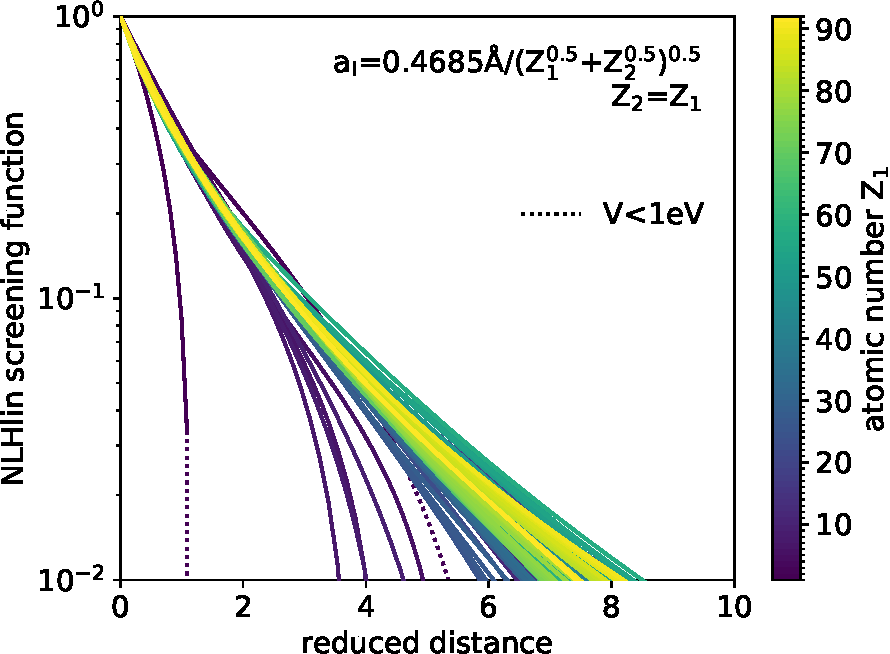
\includegraphics[scale=0.5]{nlhlin_p0.5_p0.5.pdf} ~~
    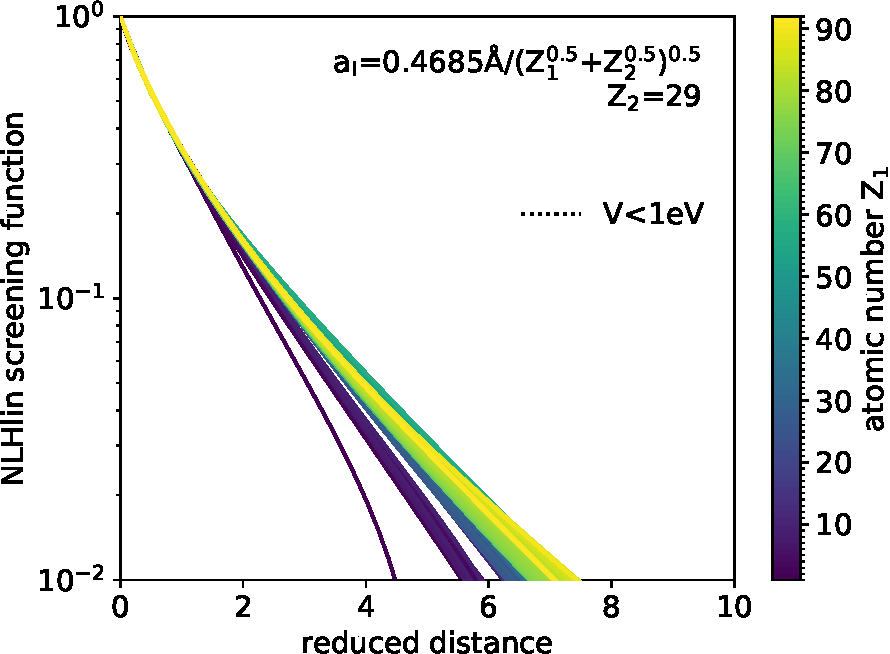
\includegraphics[scale=0.5]{nlhlin_p0.5_p0.5_Cu.pdf}
    \caption{NLHlin screening function as a function of internuclear distance scaled with the proposed screening lengths \cref{eq:sn_aNLH} for the homo-nuclear case (left) and for Cu target atoms ($Z_2=29$, right).}
    \label{fig:sn_screen_NLH}
\end{figure}

\subsection{Scattering Quantities in Terms of the Screening Function}
%%%%%%%%%%%%%%%%%%%%%%%%%%%%%%%%%%%%%%%%%%%%%%%%%%%%%%%%%%%%%%%%%%%%%
%
For a screened Coulomb potential, the equation for the distance of closest approach $R_0$ can be written in terms of reduced lengths
%
\begin{equation}
    \label{eq:sn_reduced_lengths}
    P = p/a_\mathrm{I}, \quad R = r/a_\mathrm{I}, \quad R_0 = r_0/a_\mathrm{I}, \quad T = \tau/a_\mathrm{I} ~,
\end{equation}
%
reduced energy
%
\begin{equation}
    \label{eq:sn_reduced_energy}
    \varepsilon = E \left/ \left( \frac{ M_1 + M_2 }{ M_2 }
    V_\mathrm{coul}(a_\mathrm{I}) \right) \right.
\end{equation}
%
and the screening function $\Phi(R)$ as
%
\begin{equation}
    \label{eq:sn_apsis}
    1 - \frac{ 1 }{ \varepsilon R_0 } \Phi(R_0) - \frac{ P^2 }{ R_0^2 } = 0 ~.
\end{equation}

The scattering angle in the CM system $\theta$, \cref{eq:sn_physics_theta}, and the time integral $\tau$, \cref{eq:sn_tau}, can be written as
%
\begin{equation}
    \label{eq:sn_reduced_theta}
    \pi - \theta(\varepsilon,P) = 2 \, P \int_{R_0}^\infty
        \frac{ \mathrm{d}R }{ R^2 \, g(R) }
\end{equation}
%
and
%
\begin{equation}
    \label{eq:sn_reduced_tau}
    T(\varepsilon,P) = R_0 - \int_{R_0}^\infty \left[
    \frac{ 1 }{ g(R) } - 1 \right] \mathrm{d}R.
\end{equation}
%
with
%
\begin{equation}
    \label{eq:sn_reduced_g}
    g(R) = \sqrt{ 1 - \frac{ 1 }{ \varepsilon R } \Phi(R)
        - \frac{ P^2 }{ R^2 } } .
\end{equation}

The advantage of introducing reduced parameters lies in the fact that given a universal screening function $\Phi(R)$, \crefrange{eq:sn_apsis}{eq:sn_reduced_g} depend only via \cref{eq:sn_reduced_lengths,eq:sn_reduced_energy} on the atom species.
This may be used in the development and testing of numerical algorithms, and to draw general conclusions in terms of the reduced impact parameter $P$ and energy $\varepsilon$.
We therefore use \crefrange{eq:sn_apsis}{eq:sn_reduced_g} in the following, although formulations in terms of actual lengths (in \AA) can simply be obtained by setting $a_\mathrm{I} = 1 \mathAA$ and adjusting the coefficients of $\Phi$.


\section{Calculation of the Apsis of Collision}
\label{s:apsis}
% Apsis of Collision

The apsis of collision is the distance of closest approach during a collision.
The reduced apsis of collision $R_0$ is the solution of \cref{eq:sn_apsis}.
For actually solving this equation with Newtons method, it is convenient to define the function $f(R) = R \, g^2(R)$ so that $R_0$ is the solution of:
%
\begin{equation}
    \label{eq:sn_apsis_eq}
    f(R) = R - \frac{1}{\varepsilon} \Phi(R) - \frac{P^2}{R} = 0.
\end{equation}
%
For screening functions given by a sum of exponentials, \cref{eq:sn_sum_exp}, and also for the finite-range screening function \cref{eq:sn_NLHlin}, the first derivative is always negative, \(\Phi'(R)<0\), and the second derivative is always positive, \(\Phi''(R)>0\).
It follows that \(f'(R)>0\) and \(f''(R)<0\) for all values of \(R\).
As a consequence, Newton’s method is guaranteed to converge if the initial condition \(R_{0,0}\) is chosen to the left of the solution \(R_0\) (\(R_{0,0} < R_0\)).

\subsubsection{Obtaining an initial condition}
%%%%%%%%%%%%%%%%%%%%%%%%%%%%%%%%%%%%%%%%%%%%%%
%
For purely repulsive potentials \(R_0 > P\). Therefore, \(P\) is to the left of \(R_0\), and
%
\begin{equation}
    \label{eq:sn_apsis_ic_p}
    R_0^\mathrm{(0,P)} = P
\end{equation}
%
is a possible initial condition, guaranteeing convergence of Newton’s method.
It turns out that convergence with initial condition \cref{eq:sn_apsis_ic_p} is slow for large scattering angles (i.e., small impact parameters $P$).
Therefore, a second lower boundary to $R_0$ is desirable.

For a head-on collision ($P = 0$), \cref{eq:sn_apsis_eq} reduces to
%
\begin{equation}
    \label{eq:sn_apsis_ic_eps}
    R_0^{(0,\varepsilon)} - \frac{ 1 }{ \varepsilon } \Phi(R_0^{(0,\varepsilon)}) = 0 ~.
\end{equation}
%
where we have replaced \(R\) by \(R_0^{(0,\varepsilon)}\), since we want to use this equation to obtain an alternative initial condition for $R_0$.
This equation also can be solved by iteration only.
However, it is easy to produce a table \(\varepsilon = \varepsilon(R_0^{(0,\varepsilon)})\) by calculating $\varepsilon$ from given values of $R_0^{(0,\varepsilon)}$, and to obtain a value of \(R_0^{(0,\varepsilon)}\) for a given $\varepsilon$ by interpolation in the inverse table \(R_0^{(0,\varepsilon)}(\varepsilon)\).
If the interpolation is done cubic, the derivatives \(\mathrm{d} R_0^{(0,\varepsilon)} / \mathrm{d} \varepsilon\) need to be tabulated as well. They are obtained by differentiating \cref{eq:sn_apsis_ic_eps} with respect to $\varepsilon$ and reinserting $\varepsilon$ from \cref{eq:sn_apsis_ic_eps}:
%
\begin{equation}
    \frac{ \mathrm{d} R_0^{(0,\varepsilon)} }{ \mathrm{d} \varepsilon } =
        - \frac{ (R_0^{(0,\varepsilon)})^2 }{ \Phi(R_0^{(0,\varepsilon)}) - R_0^{(0,\varepsilon)} \, \Phi'(R_0^{(0,\varepsilon)}) } ~.
\end{equation}
%
Note that $\Phi'(R) < 0$ and therefore $\mathrm{d} R_0^{(0,\varepsilon)} / \mathrm{d} \varepsilon < 0$ for all $R_0^{(0,\varepsilon)}$.%
%
\footnote{It can be shown that $\mathrm{d}^2 R_0^{(0,\varepsilon)} / \mathrm{d} \varepsilon^2 > 0$. Therefore it is advisable to use cubic rather than linear interpolation, since linear interpolation would in general overestimate $R_0^{(0,\varepsilon)}$, which could result in $R_0^{(0,\varepsilon)} > R_0$.
}

To set up the table, it seems more convenient to select values for $\varepsilon$ than for $R_0^{(0,\varepsilon)}$, since the range of \(\varepsilon\) required is known to be between the implant and the trajectory cutoff energy.
It is also possible to choose the \(\varepsilon\) limits generously, e.g. by \(\varepsilon_\mathrm{min} = 10^{-8}\) and \(\varepsilon_\mathrm{max} = 10^4\), which then would allow to use a precomputed table for all simulations.

If we desire to determine $R_0^{(0,\varepsilon)}(\varepsilon_i)$ for $\varepsilon_i = \varepsilon_\mathrm{max}/2^i$, $i = 0 \ldots n$, and $\varepsilon_\mathrm{max}/2^n \le \varepsilon_\mathrm{min} < \varepsilon_\mathrm{max}/2^{n-1}$, we can start with determining the \(R_0^{(0,\varepsilon)}\) value corresponding to \(\varepsilon_{max}\) by Newton iteration of \cref{eq:sn_apsis_eq} with $P=0$.
An initial condition for the iteration, which is to the left of the solution, is \(R_0^{(0,\varepsilon,0)} = 1/\varepsilon_\mathrm{max}\), which follows from \cref{eq:sn_apsis_ic_eps} together with \(\Phi(R_0^{(0,\varepsilon,0)}) \le 1\). Once \(R_0^{(0,\varepsilon)}(\varepsilon_\mathrm{max})\) has been determined, \(R_0^{(0,\varepsilon)}(\varepsilon_\mathrm{max}/2)\) is determined in the same way, using \(R_0^{(0,\varepsilon)}(\varepsilon_\mathrm{max})\) as initial condition, then \(R_0^{(0,\varepsilon)}(\varepsilon_\mathrm{max}/4)\) using \(R_0^{(0,\varepsilon)}(\varepsilon_\mathrm{max}/2)\) as initial condition and so on, until \(\varepsilon_\mathrm{max}/2^n \le \varepsilon_\mathrm{min}\).

$R_0^{(0,\varepsilon)}$ can also be taken as an initial condition for $P > 0$. This can be seen by
bringing the second and third term of \cref{eq:sn_apsis_eq} to the right-hand side and writing $R_0$ instead of $R$ (since the equation is fulfilled for $R = R_0$):
%
\begin{equation*}
    R_0 = \frac{1}{\varepsilon} \Phi(R_0) + \frac{P^2}{R_0} .
\end{equation*}
%
Similarly, we can rewrite \cref{eq:sn_apsis_ic_eps}
%
\begin{equation*}
    R_0^{(0,\varepsilon)} = \frac{1}{\varepsilon} \Phi(R_0^{(0,\varepsilon)}) .
\end{equation*}
%
We can easily prove that $R_0^{(0,\varepsilon)} \ge R_0$ is not possible for any $P > 0$. If $R_0^{(0,\varepsilon)} \ge R_0$ were true for some $P > 0$, because of $\mathrm{d} \Phi / \mathrm{d} R < 0$
%
\begin{equation}
    R_0 = \frac{1}{\varepsilon} \Phi(R_0) + \frac{P^2}{R_0}
        \ge \frac{1}{\varepsilon} \Phi(R_0^{(0,\varepsilon)}) + \frac{P^2}{R_0}
        = R_0^{(0,\varepsilon)} +  \frac{P^2}{R_0}
\end{equation}
%
for that $P$.
Since $P^2 / R_0 > 0$, this would mean that $R_0 > R_0^{(0,\varepsilon)}$ which contradicts the assumption $R_0^{(0,\varepsilon)} \ge R_0$.
Consequently, $R_0^{(0,\varepsilon)}$ must be smaller than $R_0$ for all $P > 0$.
So when $R_0^{(0,\varepsilon)}$ is used as an initial condition for the Newton iteration, the iteration is guaranteed to converge.

Now, as we can use both $R_0^{(0,P)}$ and $R_0^{(0,\varepsilon)}$ as initial conditions, we can choose the larger one
%
\begin{equation}
    \label{eq:sn_apsis_ic}
    R_0^{(0)} = \max( R_0^{(0,P)}, R_0^{(0,\varepsilon)} ) ,
\end{equation}
%
and we will do so as it is closer to the final solution $R_0$ than the smaller one.
\Cref{eq:sn_apsis_ic} can then be used as the initial condition in a Newton iteration
%
\begin{equation}
    \label{eq:sn_apsis_newton}
    R_0^{(i+1)} = R_0^{(i)} - f(R_0^{(i)})/f'(R_0^{(i)})
\end{equation}
%
It guarantees convergence of the iterations for screening functions with $\Phi'(R) < 0$ and $\Phi''(r) > 0$.

\subsubsection{Convergence}
%%%%%%%%%%%%%%%%%%%%%%%%%%%
%
\Cref{fig:iter-apsis} shows the number of iterations required to reach a relative accuracy of \(10^{-3}\) between the last two calculated values of \(R_0\) for the universal ZBL and the NLHlin potential.
Usually this means that the last value is accurate to \(10^{-6}\), assuming quadratic convergence has been reached.

\begin{figure}[htbp]
    \centering
    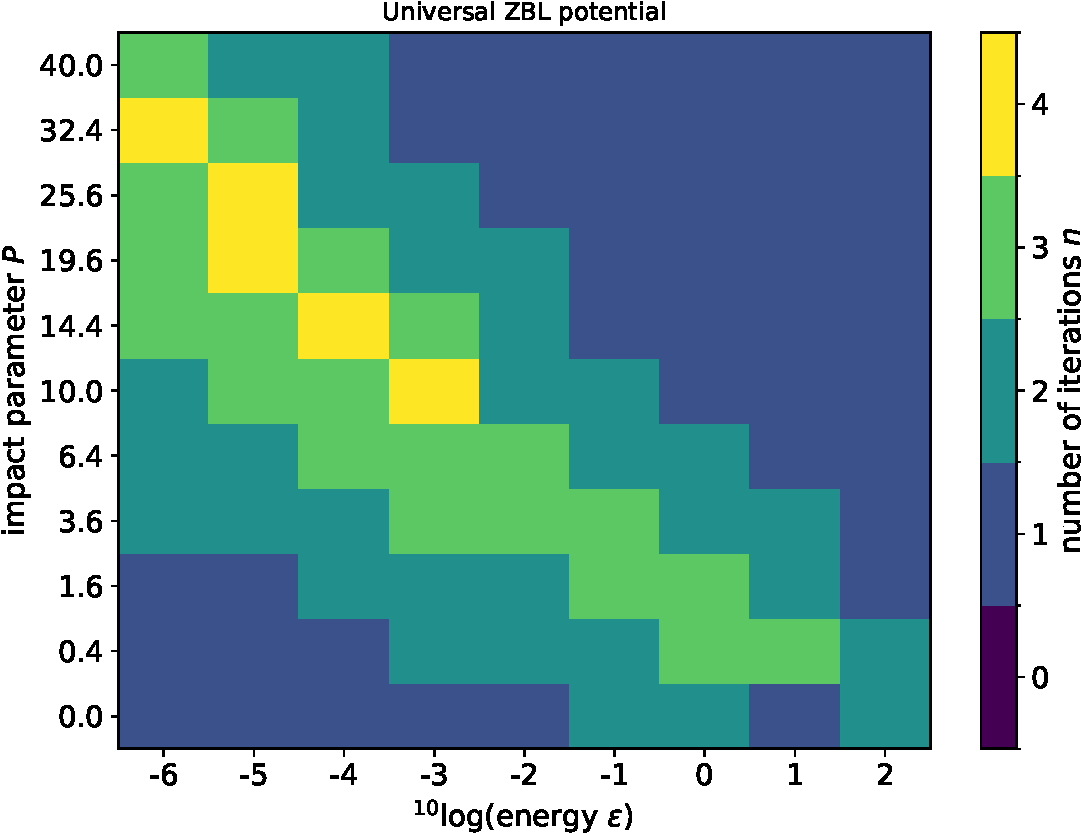
\includegraphics[scale=0.41]{ZBLuniv_iter_apsis.pdf} ~~
    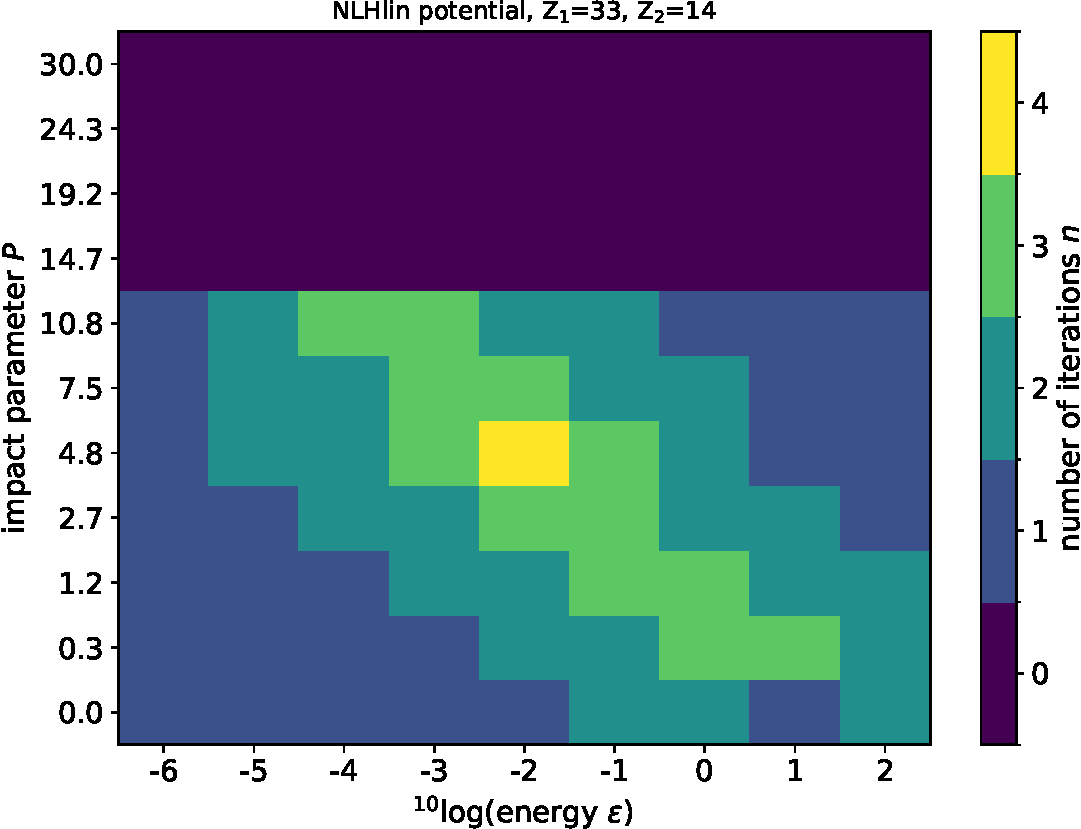
\includegraphics[scale=0.41]{NLHlin_iter_apsis.pdf}
    \caption{Number of iterations required to reach a relative accuracy of \(10^{-3}\) in \(R_0\) as a function of energy and impact parameter.
    Left: Universal ZBL potential.
    Right: NLHlin potential for As-Si using \cref{eq:sn_aNLH} as the screening length.
    The reduced impact parameters $P$ have been chosen as to cover the same range of unscaled impact parameters $p$.
    }
    \label{fig:iter-apsis}
\end{figure}

For combination of low energies and small impact parameters as well as for combinations of high energies and large impact parameters only 1-2 iterations are necessary. This is because in these cases either $R_0^{(0,P)}$ or $R_0^{(0,\varepsilon)}$ already is a good approximation to $R_0$. In other combination of $\varepsilon$ and $P$ up to 4 iterations are necessary.


\section{Calculation of the Scattering Angle in the CM System}
\label{s:cmangle}
% Scattering Angle in the CM System

\subsubsection{Change of variables}
%%%%%%%%%%%%%%%%%%%%%%%%%%%%%%%%%%%
%
The integral in \cref{eq:sn_reduced_theta} is of the form
%
\begin{equation}
    \label{eq:sn_integration_integral_R}
    \int_{R_0}^\infty F(R) \, \mathrm{d}R ~,
\end{equation}
%
where \(R_0\) is a pole of $F(R)$, which is obtained by solving \cref{eq:sn_apsis}, see Section~\ref{s:apsis}.
Having a numerically determined pole of the integrand as an integration boundary is inconvenient, so the first step of calculating the scattering integrals is to change the integration variable.
One possibility is \cite{Eck91}
%
\begin{equation}
    \label{eq:sn_transform1}
    R = \frac{ R_0 }{ (1-u^2) } ~,
\end{equation}
%
which yields
%
\begin{equation}
    \label{eq:sn_integration_integral_u1}
    \int_{R_0}^\infty F(R) \, \mathrm{d}R =
        2 R_0 \int_0^1 F \left( \frac{ R_0 }{ 1-u^2 } \right)
        \frac{ u \, \mathrm{d}u }{ (1-u^2)^2 } ~.
\end{equation}
%
With \cref{eq:sn_reduced_theta}
%
\begin{equation*}
    \pi - \theta = 2 \, P \int_{R_0}^\infty
        \frac{ \mathrm{d}R }{ R^2 \, g(R) }
\end{equation*}
%
we obtain
%
\begin{equation}
    \label{eq:sn_cmangl_legendre_theta_u}
    \pi - \theta = \frac{ 4 P }{ R_0 } \int_0^1
        \frac{ u \, \mathrm{d}u }{ g \left( \frac{ R_0 }{ 1-u^2 } \right) } ~,
\end{equation}
%
where $g(R)$ is given by \cref{eq:sn_reduced_g}
%
\begin{equation*}
    g(R) = \sqrt{ 1 - \frac{ 1 }{ \varepsilon R } \Phi(R)
        - \frac{ P^2 }{ R^2 } } ~.
\end{equation*}
%
In the following we show that the integrand is well-behaved in the interval $[0, 1]$.

\subsubsection{Rewriting the integrand}
%%%%%%%%%%%%%%%%%%%%%%%%%%%%%%%%%%%%%%%
%
It is still tricky to evaluate the integrand of \cref{eq:sn_cmangl_legendre_theta_u} near $u = 0$ (corresponding to $R \approx R_0$), since the evaluation of $g \left ( \frac{ R_0 }{ 1-u^2 } \right)$ heavily depends on the accuracy of the numerically determined value of $R_0$.
To avoid potential problems arising from this we subtract \cref{eq:sn_apsis}
%
\begin{equation*}
    1 - \frac{1}{\varepsilon R_0} \Phi(R_0) - \frac{P^2}{R_0^2} = 0
\end{equation*}

from the expression under the square root of
%
\begin{equation}
    \label{eq:sn_cmangl_legendre_g_u}
    g \left( \frac{ R_0 }{ 1-u^2 } \right) =
    \sqrt{ 1 - \frac{ 1 }{ \varepsilon R_0 }
        \Phi\left( \frac{ R_0 }{ 1-u^2 } \right) (1-u^2)
        - \frac{ P^2 }{ R_0^2 } (1-u^2)^2 } ~,
\end{equation}
%
which yields
%
\begin{equation}
    \label{eq:sn_cmangl_legendre_g_chi}
    g \left( \frac{ R_0 }{ 1-u^2 } \right) =
        \sqrt{ \frac{ R_0 }{ \varepsilon P^2 } \,
               \frac{ \Phi(R_0) - \Phi\left( \frac{ R_0 }{ 1-u^2 } \right) \, (1-u^2) }{ u^2 }
               + ( 2 - u^2 ) } ~.
\end{equation}
%
\Cref{eq:sn_cmangl_legendre_g_chi} can be rewritten
%
\begin{equation}
    \label{eq:sn_cmangl_legendre_g_G}
    g \left( \frac{ R_0 }{ 1-u^2 } \right) =
        u \frac{P}{R_0} \, G(u)
\end{equation}
%
with
%
\begin{equation}
    \label{eq:sn_cmangl_legendre_G_chi}
    G(u) = \sqrt{ \rho \, \chi(u) + (2-u^2) } ~,
\end{equation}
%
~
%
\begin{equation}
    \label{eq:sn_cmangl_legendre_chi}
    \chi(u) = \frac{ \Phi(R_0) - \Phi\left( \frac{ R_0 }{ 1-u^2 } \right) \, (1-u^2) }{ u^2 } ~,
\end{equation}
%
and
%
\begin{equation}
    \label{eq:sn_cmangl_legendre_rho}
    \rho = \frac{ R_0 }{ \varepsilon P^2 } ~.
\end{equation}

\(\chi(u)\) is well-behaved with
%
\begin{equation}
    \label{eq:sn_cmangl_legendre_chi_lim}
    \lim_{u \rightarrow 0} \chi(u) = \Phi(R_0) - R_0 \Phi'(R_0) , \qquad
    \chi(1) = \Phi(R_0) ~.
\end{equation}
%
The former is obtained by l’Hospital’s rule.
Rounding errors can be minimized by replacing \cref{eq:sn_cmangl_legendre_chi} by \cref{eq:sn_cmangl_legendre_chi_lim} for $u$ smaller than the square root of the floating point precision.
It is also easily seen that $\chi(u)$ is always positive for repulsive potentials ($\Phi'(R) < 0$ for $R \ge R_0$).
\(\chi(u)\) is plotted in \cref{fig:sn_cmangl-legendre-chi-plot} for some values of \(R_0\).
%
\begin{figure}[htbp]
    \centering
    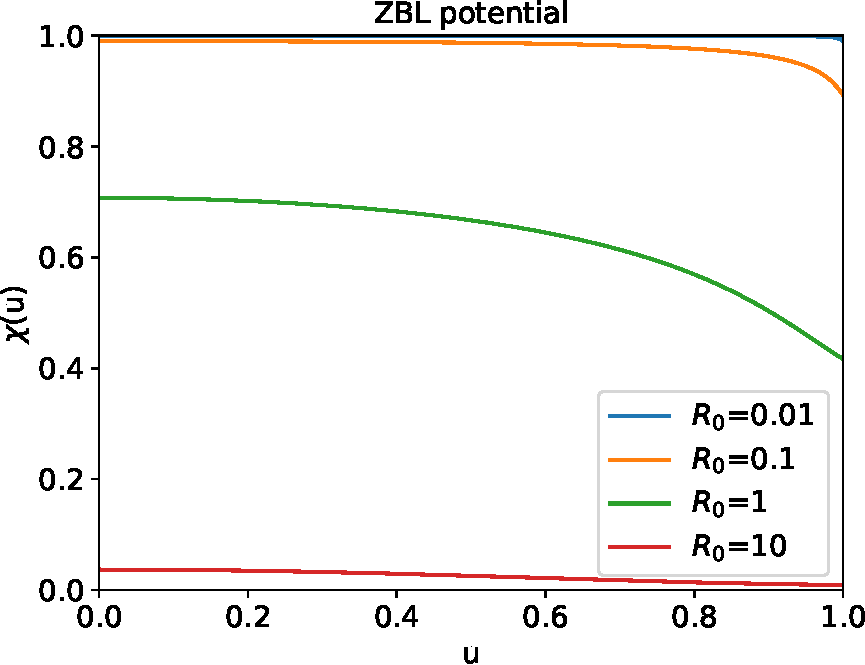
\includegraphics[scale=0.5]{chi_ZBL.pdf} ~~
    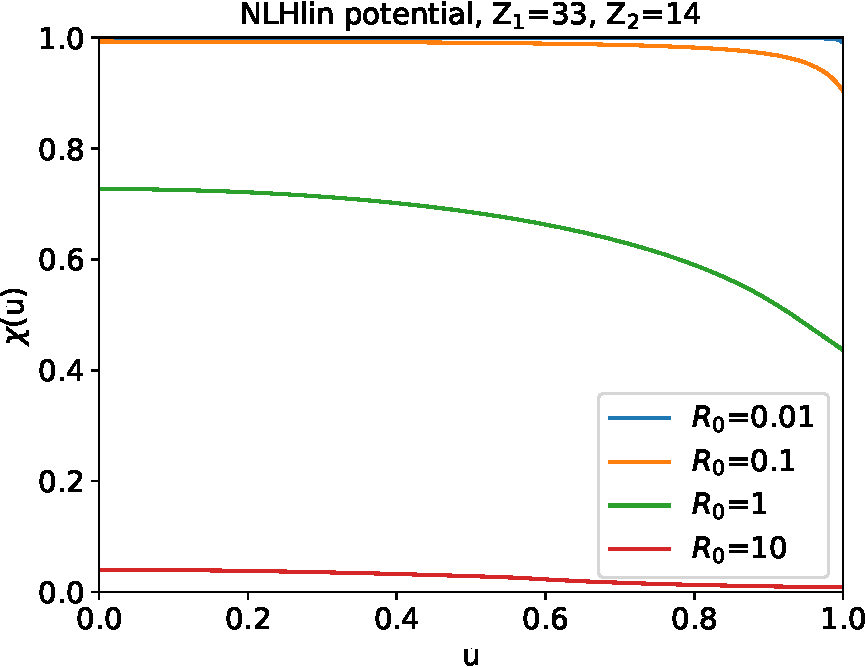
\includegraphics[scale=0.5]{chi_NLHlin_As_Si.pdf}
    \caption{Function \(\chi(u)\) according to \cref{eq:sn_cmangl_legendre_chi} for the ZBL universal potential (left) and the NLHlin potential for the atom pair As-Si (right).}
    \label{fig:sn_cmangl-legendre-chi-plot}
\end{figure}

\Cref{eq:sn_cmangl_legendre_theta_u} may now be rewritten
%
\begin{equation}
    \label{eq:sn_cmangl_legendre_theta_chi}
    \pi - \theta = 4 \int_0^1  \frac{ 1 }{ G(u) } \, \mathrm{d}u .
\end{equation}
%
The integrand has no poles, and the integral is amenable to standard methods of numerical quadrature.

$G(u)$ evaluates to infinity for $P = 0$. To avoid handling infinite values, we define
%
\begin{equation}
    \label{eq:sn_H_def}
    H(u) = P \, G(u) = \sqrt{\frac{R_0}{\varepsilon} \chi(u) + P^2 (2-u^2)} \, .
\end{equation}
%
Then \cref{eq:sn_cmangl_legendre_theta_chi} can be rewritten
%
\begin{equation}
    \label{eq:sn_cmangl_legendre_theta_H}
    \pi - \theta = 4 P \int_0^1  \frac{ 1 }{ H(u) } \, \mathrm{d}u .
\end{equation}
%
Apart from showing $\theta = \pi$, this explicitly shows that $\pi - \theta \sim P$ for small impact parameters.

\subsubsection{Integration using Gauss-Legendre quadrature}
%%%%%%%%%%%%%%%%%%%%%%%%%%%%%%%%%%%%%%%%%%%%%%%%%%%%%%%%%%%
%
Using Gauss-Legendre quadrature, we can approximate \cref{eq:sn_cmangl_legendre_theta_chi} by
%
\begin{equation}
    \label{eq:sn_cmangl_legendre_theta_chi_approx_plain}
    \pi - \theta \approx
        4 \sum_{i=1}^n \frac{ \tilde{w}_i }{ G(\tilde{u}_i) }
\end{equation}
%
with \(\tilde{u}_i\) and \(\tilde{w}_i\) from \cref{eq:sn_legendre_transform}. With $a=0$ and $b=1$ they read
%
\begin{equation}
    \label{eq:sn_gauss_legendre_transform_infinite}
    \tilde{u}_i = \frac{ u_i + 1 }{ 2 }, \qquad
    \tilde{w} = \frac{ w_i }{ 2 }.
\end{equation}

\Cref{eq:sn_cmangl_legendre_theta_chi_approx_plain}, however, has the problem that $\theta$ does not tend to zero exactly as $P \rightarrow \infty$ or $\varepsilon \rightarrow \infty$, since the right-hand side only approximates $\pi$.
Note that for \(\rho \rightarrow 0\) the integral in \cref{eq:sn_cmangl_legendre_theta_chi} becomes
%
\begin{equation}
    \label{eq:sn_cmangl_legendre_pi}
    \int_0^1 \frac{ 1 }{ \sqrt{ 2-u^2 } } \, \mathrm{d}u = \frac{ \pi }{ 4 } ~,
\end{equation}
%
and \(\theta \rightarrow 0\) as it should.
Since the integrand is not a polynomial, the Legendre approximation of the integral will not exactly evaluate to \(\pi/4\), and \cref{eq:sn_cmangl_legendre_theta_chi_approx_plain} will not tend to $\pi$ as \(\rho \rightarrow 0\).
This may be fixed by scaling the integral to the correct value of \(\pi/4\):
%
\begin{equation}
    \label{eq:sn_cmangl_legendre_theta_chi_approx}
    \pi - \theta \approx
        \frac{ \pi }{ \pi_\mathrm{num}/4 }
        \sum_{i=1}^n \frac{ \tilde{w}_i }{ G(\tilde{u}_i) }
\end{equation}
%
with
%
\begin{equation}
    \label{eq:sn_cmangl_legendre_pinum}
    \frac{\pi_\mathrm{num}}{4} =
        \sum_{i=1}^n \frac{ \tilde{w}_i  }{ \sqrt{ 2-\tilde{u}_i^2 } }
\end{equation}
%
Since the sum in \cref{eq:sn_cmangl_legendre_theta_chi_approx} evaluates to \(\pi_\mathrm{num}/4\) for \(\rho \rightarrow 0\), $\pi - \theta$ tends to $\pi$ and \(\theta \rightarrow 0\).
At the same time, for \(\rho \rightarrow \infty\) (i.e., for $\varepsilon \rightarrow 0$ or $P \rightarrow 0$), $G(u) \rightarrow \infty$, and the sum in \cref{eq:sn_cmangl_legendre_theta_chi_approx} goes to zero and \(\theta \rightarrow \pi\) as it should.

In terms of the function $H(u)$, \cref{eq:sn_H_def}, \cref{eq:sn_cmangl_legendre_theta_chi_approx} reads
%
\begin{equation}
    \label{eq:sn_cmangl_legendre_theta_H_approx}
    \pi - \theta \approx
        \frac{ \pi }{ \pi_\mathrm{num}/4 }  \,
        P \sum_{i=1}^n \frac{ \tilde{w}_i }{ H(\tilde{u}_i) }
\end{equation}

One can also apply this correction to the Gauss-Legendre approximation of \cref{eq:sn_cmangl_legendre_theta_u}:
%
\begin{equation*}
    %\label{eq:sn_cmangl_legendre_theta_g_approx}
    \pi - \theta \approx
        \frac{ \pi }{ \pi_\mathrm{num}/4 } \, \frac{ P }{ R_0 }
        \sum_{i=1}^n
        \frac{ \tilde{w}_i \tilde{u}_i
        }{ g \left( \frac{ R_0 }{ 1-\tilde{u}_i^2 } \right) } \, .
\end{equation*}
%
This expression is not numerically equivalent to \cref{eq:sn_cmangl_legendre_theta_chi_approx}.
It does not require the evaluation of \(\Phi(R_0)\), which might represent a noticable saving of computation time if few abscissas are used.
For few abscissas, the results are very similar.
With increasing number of abscissas, the results are increasingly dependent on the accuracy of the apsis \(R_0\).
The term under the square root of $g(\frac{R_0}{1-u^2})$, \cref{eq:sn_cmangl_legendre_g_chi}, or $G(u)$, \cref{eq:sn_cmangl_legendre_G_chi}, may even become negative, if the accuracy of \(R_0\) is low and the number of abscissas is large.

\subsubsection{Modifications for finite-range screened Coulomb potentials}
%%%%%%%%%%%%%%%%%%%%%%%%%%%%%%%%%%%%%%%%%%%%%%%%%%%%%%%%%%%%%%%%%%%%%%%%%
%
If $\Phi(R) = 0$ for $R$ larger than some $R_\mathrm{max}$,
%
\begin{equation}
    \Phi(R) = 0 \quad \text{for} \quad R \ge R_\mathrm{max}
\end{equation}
%
then for $P \ge R_\mathrm{max}$ we trivially have $\theta = 0$.
Otherwise the integral in \cref{eq:sn_reduced_theta} must be divided in two parts:
%
\begin{equation}
    \label{eq:sn_reduced_theta_finite}
    \pi - \theta =
        2 \, P \int_{R_0}^\infty \frac{ \mathrm{d}R }{ R^2 \, g(R) } =
        2 \, P \int_{R_0}^{R_\mathrm{max}} \frac{ \mathrm{d}R }{ R^2 \, g(R) } +
        2 \, P \int_{R_\mathrm{max}}^{\infty} \frac{ \mathrm{d}R }{ R^2 \, g(R) } ~.
\end{equation}
%
The second term on the right-hand side may be evaluated analytically using $g(R)$ with $\Phi(R) = 0$
%
\begin{equation}
    \label{eq:sn_g_phi=0}
    g(R) = \sqrt{ 1 - \frac{ P^2 }{ R_0^2 }}
\end{equation}
%
and \cite[2.275.4]{Gra80}
%
\begin{equation}
    \label{eq:sn_reduced_theta_finite_2}
    2 \, P \int_{R_\mathrm{max}}^{\infty} \frac{ \mathrm{d}R }{ R^2 \, g(R) } =
        2 \, P \int_{R_\mathrm{max}}^{\infty}
            \frac{ \mathrm{d}R }{ R^2 \sqrt{ 1 - \frac{P^2}{R^2}} } =
        2 \arcsin \frac{P}{R_\mathrm{max}} ~.
\end{equation}
%
Note that for $R_\mathrm{max} \rightarrow \infty$, this term vanishes.

Applying the substitution \cref{eq:sn_transform1} to the remaining integral yields
%
\begin{equation}
    \pi - \theta =
        4 \int_0^{u_\mathrm{max} } \frac{ \mathrm{d}u }{G(u)} +
        2 \arcsin \frac{P}{R_\mathrm{max}}
\end{equation}
%
with
%
\begin{equation}
    \label{eq:sn_umax}
    u_\mathrm{max} = \sqrt{ 1 - \frac{ R_0 }{ R_\mathrm{max} } } ~,
\end{equation}

The integral can be evaluated by Gauss-Legendre quadrature
%
\begin{equation}
    \label{eq:sn_cmangl_legendre_theta_chi_finite_approx_plain}
    \pi - \theta =
        4 \sum_{i=1}^n \frac{ \tilde{w}_i }{G(\tilde{u}_i)} +
        2 \arcsin \frac{P}{R_\mathrm{max}}
\end{equation}
%
with
%
\begin{equation}
    \label{eq:sn_gauss_legendre_transform_finite}
    \tilde{u}_i = u_\mathrm{max} \frac{ u_i + 1 }{ 2 }, \qquad
    \tilde{w}_i = u_\mathrm{max} \frac{ w_i }{ 2 }
\end{equation}
%
which follows from \cref{eq:sn_legendre_transform} with $a=0$ and $b=u_\mathrm{max}$.

As with \cref{eq:sn_cmangl_legendre_theta_chi_approx_plain}, for numerical reasons $\rho \rightarrow 0$ might not exactly result in $\theta \rightarrow 0$ as it should.
Unlike for infinite-range potentials, this does not happen for $P \rightarrow \infty$, because for $P > R_\mathrm{max}$ we have the trivial solution $\theta = 0$.
Also for $P = R_\mathrm{max}$ there is no problem because the first term evaluates to zero and the second term evaluates to $\pi$.
But for very high energies $\varepsilon \rightarrow \infty$ and not too small $P$, $\rho$ can become very small.
In that case,
%
\begin{equation}
    \lim_{\varepsilon \rightarrow \infty} \left[
        4 \int_{0}^{u_\mathrm{max}} \frac{ \mathrm{d} u}{G(u)} \right] =
        4 \int_{0}^{u_\mathrm{max}} \frac{ \mathrm{d} u}{\sqrt{2-u^2}} =
        4 \arcsin \frac{u_\mathrm{max}}{\sqrt{2}} = 2 \arccos \frac{R_0}{R_\mathrm{max}}
\end{equation}
%
One can therefore numerically correct \cref{eq:sn_cmangl_legendre_theta_chi_finite_approx_plain} by
%
\begin{equation}
    \label{eq:sn_cmangl_legendre_theta_chi_finite}
    \pi - \theta =
        2 \, \frac{\arccos (R_0 / R_\mathrm{max})}{\frac{1}{2} \arccos_\mathrm{num}} \,
            \sum_{i=1}^n \frac{ \tilde{w}_i }{G( \tilde{u}_i)}
        + 2 \arcsin \frac{P}{R_\mathrm{max}}
\end{equation}
%
with
%
\begin{equation}
    \frac{1}{2} \arccos_\mathrm{num} =
        \sum_{i=1}^n \frac{ \tilde{w}_i }{\sqrt{2 - \tilde{u}_i^2}} \, .
\end{equation}
$\theta$ tends to 0 as $\varepsilon \rightarrow \infty$, since $\rho \rightarrow 0$ and $R_0 \rightarrow P$, and $\arccos x + \arcsin x = \pi/2$. Contrary to $\pi_\mathrm{num}$, \cref{eq:sn_cmangl_legendre_pinum}, the second sum in \cref{eq:sn_cmangl_legendre_theta_chi_finite} depends on $\varepsilon$ and $P$ via $u_\mathrm{max}$ and $R_0$.

For $P = 0$, $\rho \rightarrow \infty$ and therefore $G(u) \rightarrow \infty$, and both terms vanish. So there is no problem in evaluating \cref{eq:sn_cmangl_legendre_theta_chi_finite} for head-on collisions.
Contrary to $\pi_\mathrm{num}/4$, \cref{eq:sn_cmangl_legendre_pinum}, $\frac{1}{2} \arccos_\mathrm{num}$ depends on $\varepsilon$ and $P$ via $u_\mathrm{max}$ and $R_0$.

In terms of the function $H(u)$, \cref{eq:sn_H_def}, \cref{eq:sn_cmangl_legendre_theta_chi_finite} reads
%
\begin{equation}
    \label{eq:sn_cmangl_legendre_theta_H_finite}
    \pi - \theta =
        2 \, \frac{\arccos (R_0 / R_\mathrm{max})}{\frac{1}{2}\arccos_\mathrm{num}} \,
        P \sum_{i=1}^n \frac{ \tilde{w}_i }{H( \tilde{u}_i)}
        + 2 \arcsin \frac{P}{R_\mathrm{max}} \, .
\end{equation}
%
Also for finite-range interatomic potentials, $\pi - \theta \sim P$ for small P, since $\arcsin x \approx x$ for small $x$.

\subsubsection{Convergence}
%%%%%%%%%%%%%%%%%%%%%%%%%%%
%
\begin{figure}[htbp]
    \centering
    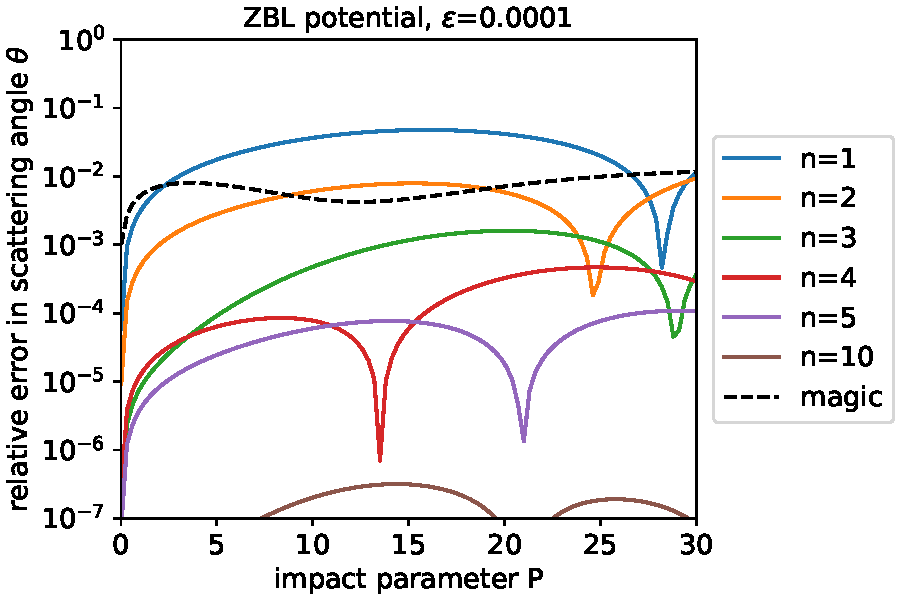
\includegraphics[scale=0.5]{error_legendre_theta_eps1e-4_zbl.pdf} ~~
    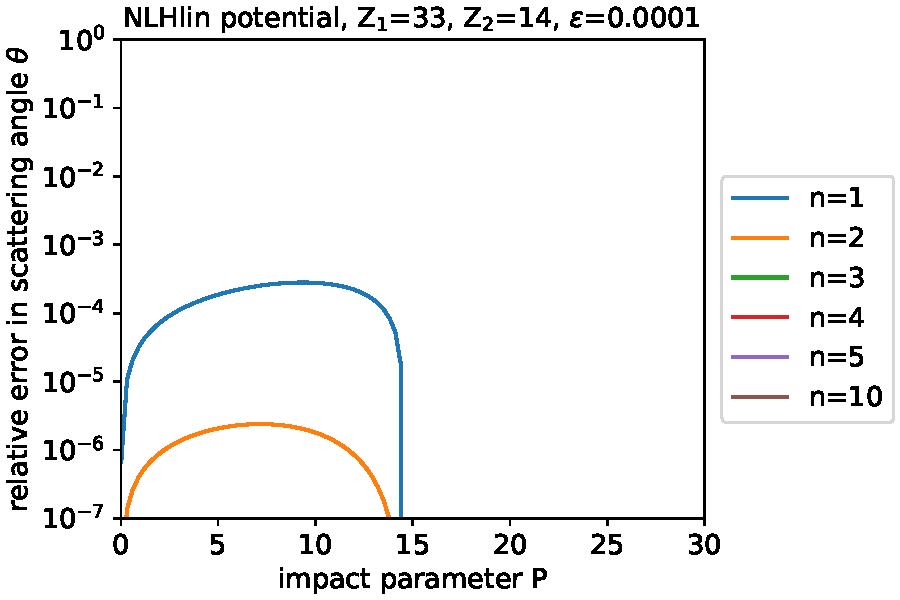
\includegraphics[scale=0.5]{error_legendre_theta_eps1e-4_nlhlin.pdf} \\ \smallskip
    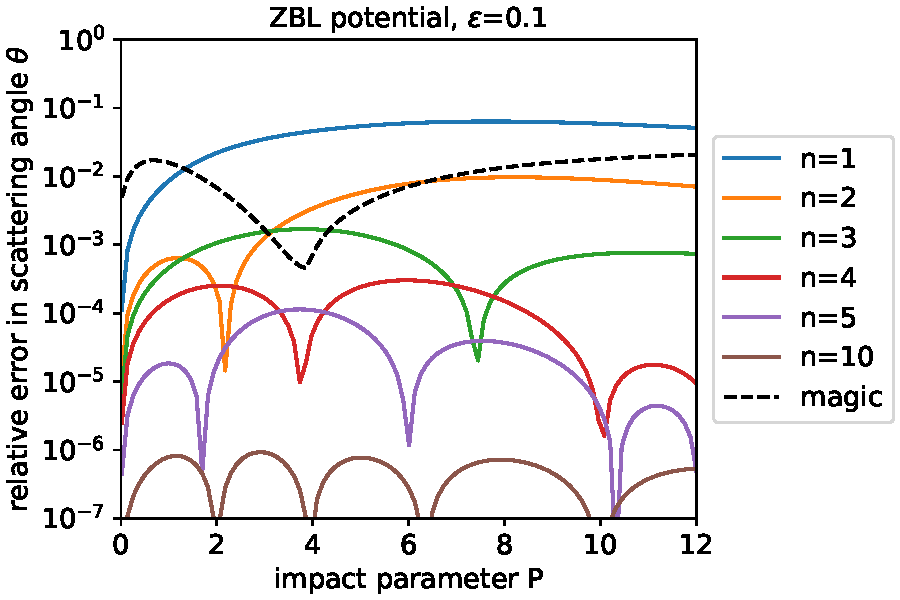
\includegraphics[scale=0.5]{error_legendre_theta_eps0.1_zbl.pdf} ~~
    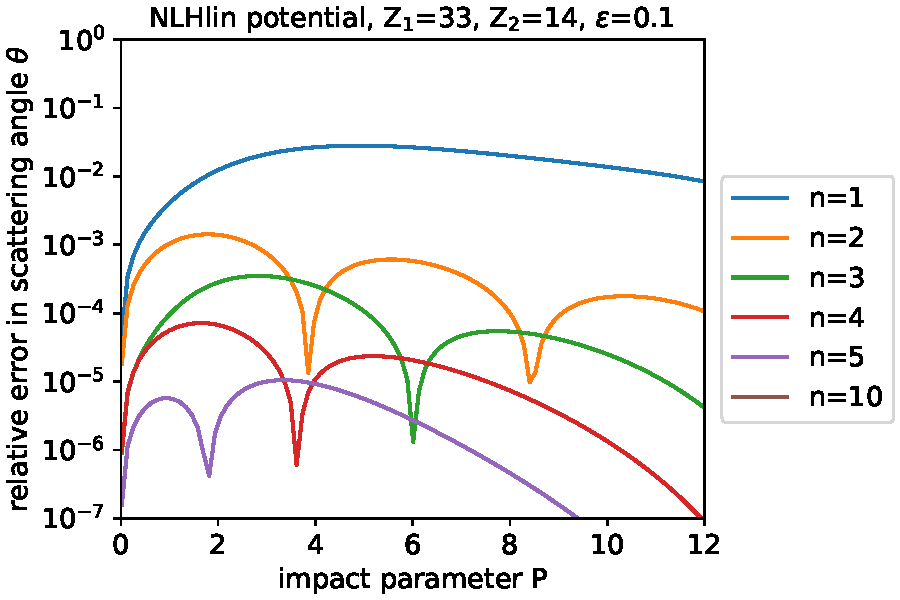
\includegraphics[scale=0.5]{error_legendre_theta_eps0.1_nlhlin.pdf} \\ \smallskip
    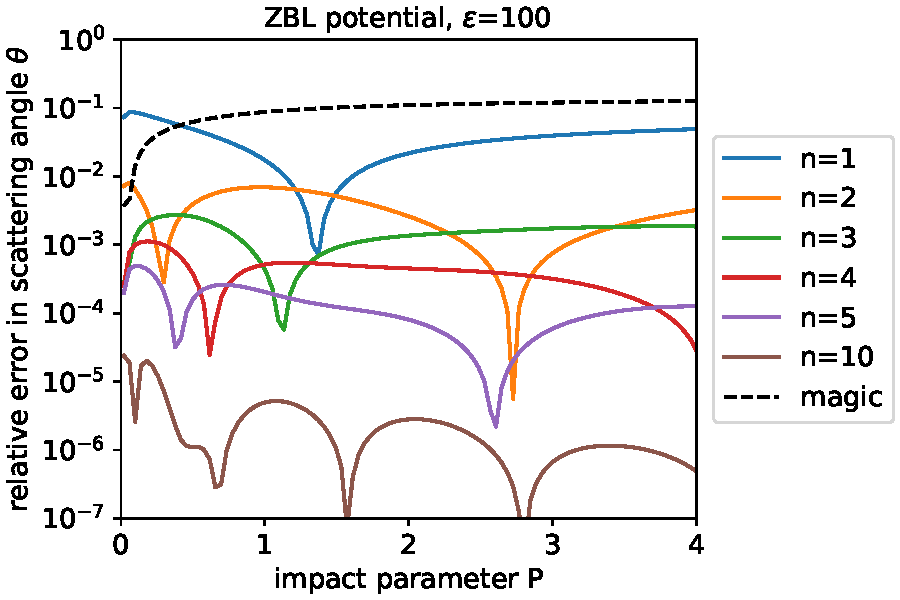
\includegraphics[scale=0.5]{error_legendre_theta_eps100_zbl.pdf} ~~
    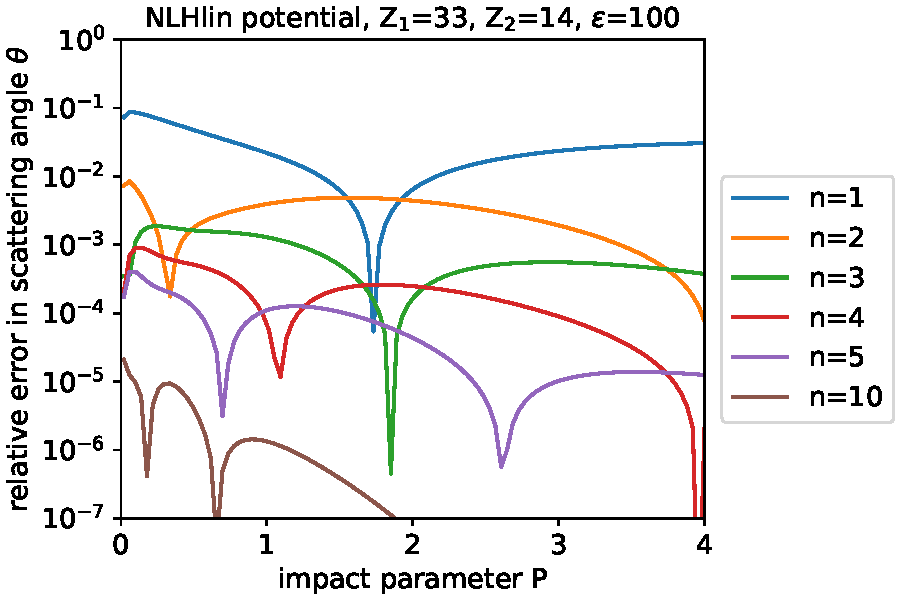
\includegraphics[scale=0.5]{error_legendre_theta_eps100_nlhlin.pdf}
    \caption{Relative errors in \(\theta\) of n-point Gauss-Legendre quadrature as a function of reduced impact parameter for three energies using \cref{eq:sn_cmangl_legendre_theta_chi_finite} with the number of abscissae $n=1$,2, 3, 4, 5, and 10.
        As interatomic potentials the universal ZBL potential (left) and the NLHlin potential for $Z_1=33$ and $Z_2=14$ were used together with a screening length given by \cref{eq:sn_aNLH}.
        For the ZBL potential the results of Biersack's magic formula \cite{Bie80} (check!) are also included with dashed lines.
        The reference simulations were evaluated using \cref{eq:sn_cmangl_legendre_theta_chi_finite} with 32-point Gauss-Legendre quadrature.
        The relative accuracy of the apsis is better than \(10^{-3}\).}
    \label{fig:error-legendre-theta}
\end{figure}
%
In \cref{fig:error-legendre-theta}, the relative errors in \(\theta\) as calculated by \cref{eq:sn_cmangl_legendre_theta_chi_finite} are shown as a function of reduced impact parameter $P$ for reduced energies \(\varepsilon = 10^{-4}\), \(\varepsilon = 10^{-1}\), and \(\varepsilon = 100\), and different numbers of abscissae $n$ in the Gauss-Legendre quadrature.
The results for the ZBL potential are shown in the left column, while those for the NLHlin potential are found in the right column.
For the ZBL potential, the result of Biersacks magic formula \cite{Bie80} (check!) are also shown.
Notably, the accuracy of the magic formula, about 1~\%, is already reached with only $n=2$ abscissae in the Gauss-Legendre quadrature.
An accuracy 10$^{-4}$--10$^{-3}$ is reached with $n = 4$.
For the NLHlin potential, convergence is even faster in general.

\textbf{TODO: Magic formula}

\section{Calculation of the Time Integral}
\label{s:time}
% Time Integral

\subsubsection{Infinite-range screened Coulomb potentials}
%%%%%%%%%%%%%%%%%%%%%%%%%%%%%%%%%%%%%%%%%%%%%%%%%%%%%%%%%%
%
The integral in \cref{eq:sn_reduced_tau} for the calculation of the time integral is also of the form \cref{eq:sn_integration_integral_R}. Applying the same substitution of variables \cref{eq:sn_transform1} to \cref{eq:sn_reduced_tau}, one obtains
%
\begin{equation}
    \label{eq:sn_tau_u}
    T = R_0 - 2 R_0 \int_0^1
        \left[ \frac{ 1 }{ g \left( \frac{ R_0 }{ 1-u^2 } \right) } - 1 \right]
        \frac{ u }{ (1-u^2)^2 }
        \, \mathrm{d}u
\end{equation}
%
with $g(\frac{R_0}{1-u^2})$ as given by \cref{eq:sn_cmangl_legendre_g_u}.
Combining the two terms in brackets in \cref{eq:sn_tau_u} and multiplying numerator and denominator with $1 + g(\frac{R_0}{1-u^2})$ gives
%
\begin{equation}
    \label{eq:sn_tau_u1}
    T = R_0 - 2 R_0 \int_0^1
        \frac{ 1 - g^2 \left( \frac{ R_0 }{ 1-u^2 } \right) }{
               g \left( \frac{ R_0 }{ 1-u^2 } \right)
               \left[ 1 + g \left( \frac{ R_0 }{ 1-u^2 } \right) \right] }
        \frac{ u }{ (1-u^2)^2 }
        \, \mathrm{d}u .
\end{equation}
%
Inserting \cref{eq:sn_cmangl_legendre_g_u} in the numerator and \cref{eq:sn_cmangl_legendre_g_G} in the demoninator, and using \crefrange{eq:sn_cmangl_legendre_G_chi}{eq:sn_cmangl_legendre_rho} yields
%
\begin{equation}
    \label{eq:sn_tau_G}
    T = R_0 - 2 P \int_0^1
        \frac{ 1 + \rho \, \frac{ 1 }{ 1-u^2 } \, \Phi \left( \frac{R_0}{1-u^2} \right) }{
               G(u) \left[ 1 + u \frac{P}{R_0} G(u) \right] }
        \, \mathrm{d}u ~.
\end{equation}
%
Note that the term $\frac{ 1 }{ 1-u^2 } \, \Phi \left( \frac{R_0}{1-u^2} \right)$ does not diverge if $R\, \Phi(R) \rightarrow 0$ as $R \rightarrow \infty$, in other words, if $\Phi(R)$ decays faster that $1/R$.

Using Gauss-Legendre quadrature, the time integral may be approximated by
%
\begin{equation}
    \label{eq:sn_tau_G_legendre}
    T = R_0 - 2 P \sum_{i-1}^n \tilde{w}_i
        \frac{ 1 + \rho \, \frac{ 1 }{ 1-\tilde{u}_i^2 } \, \Phi \left( \frac{R_0}{1-\tilde{u}_i^2} \right) }{
        G(\tilde{u}_i) \left[ 1 + \tilde{u}_i \frac{P}{R_0} G(\tilde{u}_i) \right] } ~.
\end{equation}
%
with $\tilde{u}_i$ and $\tilde{w}_i$ defined in \cref{eq:sn_gauss_legendre_transform_infinite}.
In terms of the function $H(u)$, \cref{eq:sn_H_def}, \cref{eq:sn_tau_G_legendre} reads
%
\begin{equation}
    \label{eq:sn_tau_H_legendre}
        T = R_0 - 2 \sum_{i-1}^n \tilde{w}_i
        \frac{ P^2 + \frac{R_0}{\varepsilon} \, \frac{ 1 }{ 1-\tilde{u}_i^2 } \, \Phi \left( \frac{R_0}{1-\tilde{u}_i^2} \right) }{
        H(\tilde{u}_i) \left[ 1 + \frac{\tilde{u}_i}{R_0} H(\tilde{u}_i) \right] } ~.
\end{equation}
%
which explicitly shows that the second term does not vanish for $P \rightarrow 0$.

\subsubsection{Finite-range screened Coulomb potentials}
%%%%%%%%%%%%%%%%%%%%%%%%%%%%%%%%%%%%%%%%%%%%%%%%%%%%%%%%
%
For finite-range screened Coulomb potentials we are interested only in $P < R_\mathrm{max}$ since for $\theta = 0$ the outgoing asymptote is identical with the incoming asymptote independent of the time integral.
Like for the scattering angle, we split the integral in \cref{eq:sn_reduced_tau} in two parts:
%
\begin{equation}
    \label{eq:sn_reduced_tau_finite}
    T = R_0 -
        \int_{R_0}^{R_\mathrm{max}} \left[ \frac{ 1 }{ g(R) } - 1 \right] \mathrm{d}R -
        \int_{R_\mathrm{max}}^\infty \left[ \frac{ 1 }{ g(R) } - 1 \right] \mathrm{d}R ~.
\end{equation}
%
The second integral may be evaluated analytically using \cref{eq:sn_g_phi=0}
%
\begin{equation}
    T = R_0 -
        (R_\mathrm{max} - \sqrt{ R_\mathrm{max}^2 - P^2 }) -
        \int_{R_\mathrm{max}}^\infty \left[ \frac{ 1 }{ g(R) } - 1 \right] \mathrm{d}R ~.
\end{equation}

Applying the substitution \cref{eq:sn_transform1} to the remaining integral, using the identity
%
\begin{equation*}
    \frac{1}{g} - 1 = \frac{1-g}{g} = \frac{1-g^2}{g(1+g)}
\end{equation*}
%
and Eqs.~(\ref{eq:sn_cmangl_legendre_g_u}), (\ref{eq:sn_cmangl_legendre_g_G}), (\ref{eq:sn_cmangl_legendre_G_chi}), and (\ref{eq:sn_cmangl_legendre_rho})
we obtain
%
\begin{equation}
    \label{eq:sn_reduced_tau_finite_G_legendre}
    T = R_0 -
        (R_\mathrm{max} - \sqrt{ R_\mathrm{max}^2 - P^2 }) - 2 P \int_0^{u_\mathrm{max}}
        \frac{ 1 + \rho \, \frac{ 1 }{ 1-u^2 } \, \Phi \left( \frac{R_0}{1-u^2} \right) }{
            G(u) \left[ 1 + u \frac{P}{R_0} G(u) \right] }
        \, \mathrm{d}u \\
\end{equation}
%
with $u_\mathrm{max}$ as defined in \cref{eq:sn_umax}.

Using Gauss-Legendre quadrature, the time integral may finally be approximated by
%
\begin{equation}
    \label{eq:sn_cmangl_legendre_tau_chi_finite}
    T = R_0 - R_\mathrm{max} + \sqrt{ R_\mathrm{max}^2 - P^2 } -
    2 P \sum_{i=1}^n \tilde{w}_i
    \frac{ 1 + \rho \, \frac{ 1 }{ 1-\tilde{u}_i^2 } \, \Phi \left( \frac{R_0}{1-\tilde{u}_i^2} \right) }{
        G(\tilde{u}_i) \left[ 1 + \tilde{u}_i \frac{P}{R_0} G(\tilde{u}_i) \right] } ~.
\end{equation}
%
with $\tilde{u}_i$ and $\tilde{w}_i$ defined in \cref{eq:sn_gauss_legendre_transform_finite}.
In terms of the function $H(u)$, \cref{eq:sn_H_def}, \cref{eq:sn_cmangl_legendre_tau_chi_finite} reads
%
\begin{equation}
    \label{eq:sn_cmangl_legendre_tau_H_finite}
    T = R_0 - R_\mathrm{max} + \sqrt{ R_\mathrm{max}^2 - P^2 } -
        2 \sum_{i=1}^n \tilde{w}_i
        \frac{ P^2 + \frac{R_0}{\varepsilon} \, \frac{ 1 }{ 1-\tilde{u}_i^2 } \, \Phi \left( \frac{R_0}{1-\tilde{u}_i^2} \right) }{
        H(\tilde{u}_i) \left[ 1 + \frac{\tilde{u}_i}{R_0} H(\tilde{u}_i) \right] } ~.
\end{equation}


\subsubsection{Convergence}
%%%%%%%%%%%%%%%%%%%%%%%%%%%
%
\begin{figure}[htbp]
    \centering
    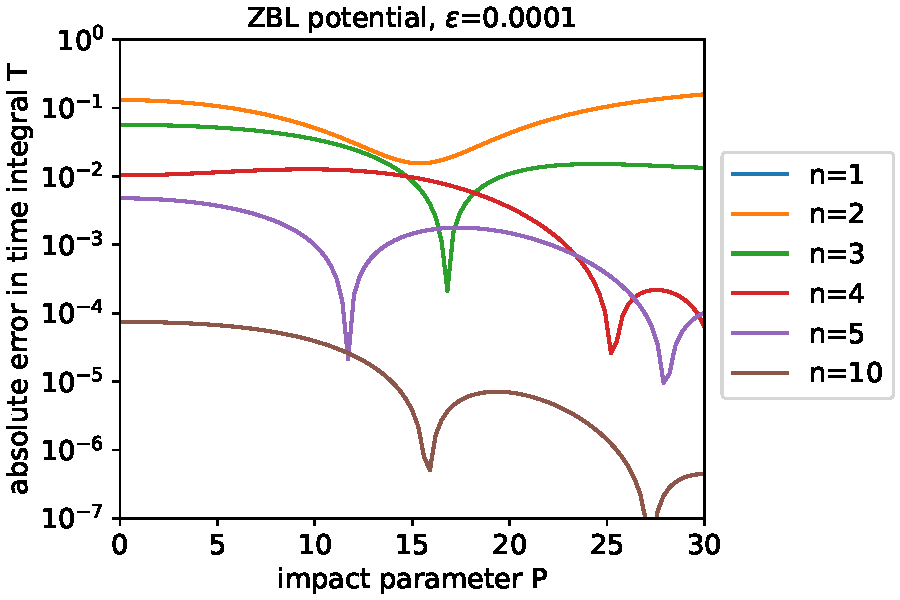
\includegraphics[scale=0.5]{error_legendre_tau_eps1e-4_zbl.pdf} ~~
    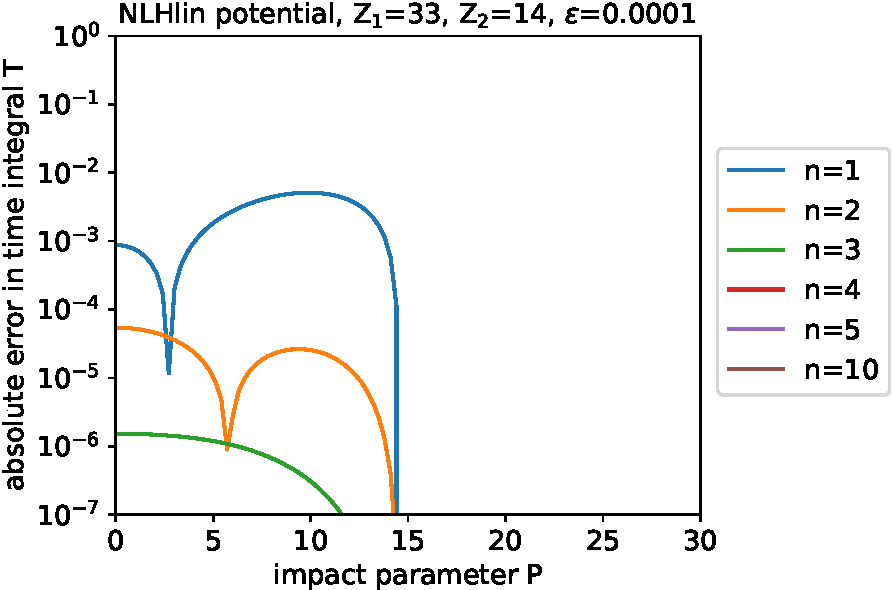
\includegraphics[scale=0.5]{error_legendre_tau_eps1e-4_nlhlin.pdf} \\ \smallskip
    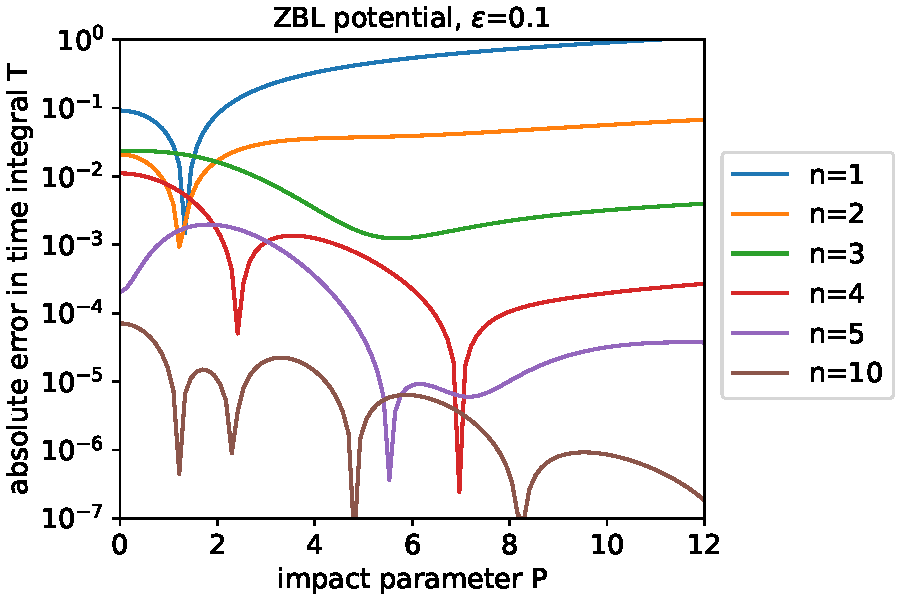
\includegraphics[scale=0.5]{error_legendre_tau_eps0.1_zbl.pdf} ~~
    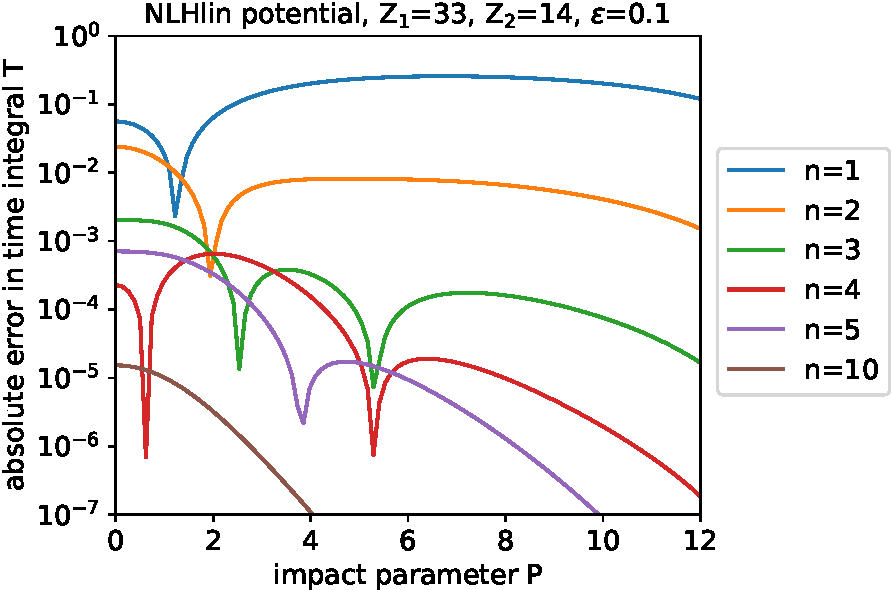
\includegraphics[scale=0.5]{error_legendre_tau_eps0.1_nlhlin.pdf} \\ \smallskip
    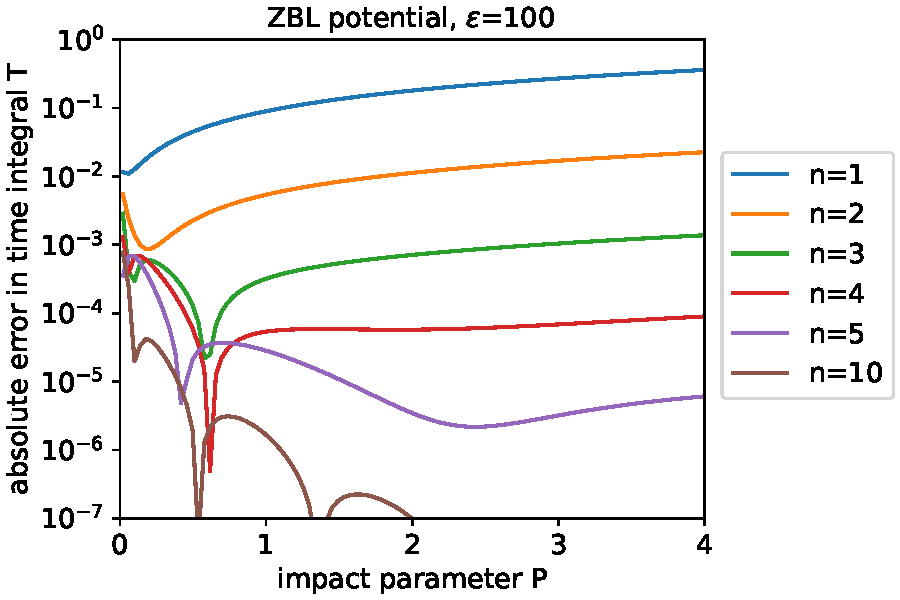
\includegraphics[scale=0.5]{error_legendre_tau_eps100_zbl.pdf} ~~
    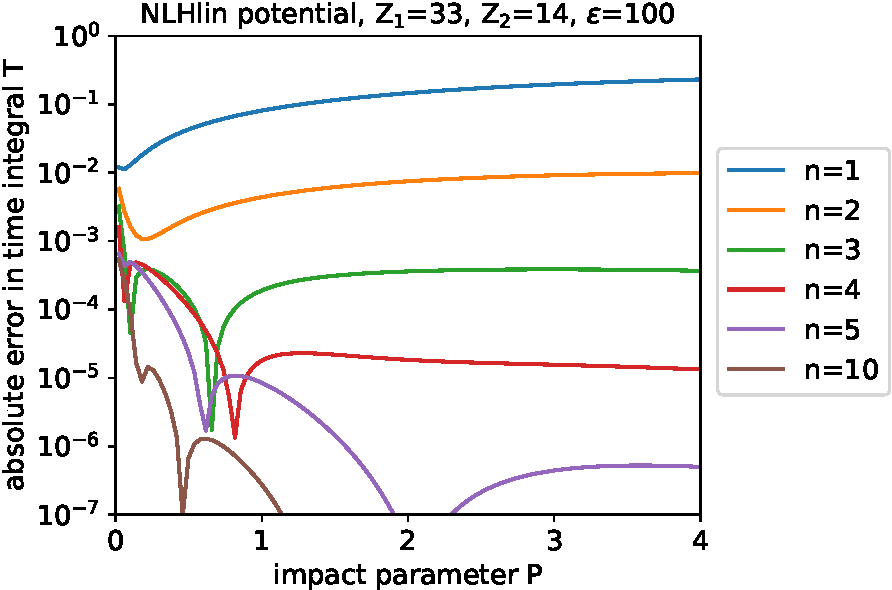
\includegraphics[scale=0.5]{error_legendre_tau_eps100_nlhlin.pdf}
    \caption{Relative errors in the time integral \(T = \tau/a_\mathrm{I}\) of n-point Gauss-Legendre quadrature as a function of reduced impact parameter for three energies using \cref{eq:sn_cmangl_legendre_tau_chi_finite} with the number of abscissae $n=1$,2, 3, 4, 5, and 10.
        As interatomic potentials the universal ZBL potential (left) and the NLHlin potential for $Z_1=33$ and $Z_2=14$ were used together with a screening length $a_\mathrm{I}$ given by \cref{eq:sn_aNLH}.
        The reference simulations were evaluated using \cref{eq:sn_cmangl_legendre_tau_chi_finite} with 32-point Gauss-Legendre quadrature.
        The relative accuracy of the apsis is better than \(10^{-3}\).}
    \label{fig:error-legendre-tau}
\end{figure}
%
In \cref{fig:error-legendre-tau}, the relative errors in \(T = \tau/a_\mathrm{I}\) as calculated by \cref{eq:sn_cmangl_legendre_tau_chi_finite} are shown as a function of reduced impact parameter $P$ for reduced energies \(\varepsilon = 10^{-4}\), \(\varepsilon = 10^{-1}\), and \(\varepsilon = 100\), and different numbers of abscissae $n$ in the Gauss-Legendre quadrature.
The results for the ZBL potential are shown in the left column, while those for the NLHlin potential are found in the right column.
An accuracy of at least 1\% is reached with $n = 4$.
For the NLHlin potential, convergence is even faster in general.

In summary, 4-point Gauss-Legendre quadrature allows the calculation of the scattering angle with an accuracy of  better than 10$^{-3}$ and the calculation of the time integral with an accuracy of better than 1\%.
Using the same number of abscissae for the calculation of both quantities has the advantage that the $\Phi \left( \frac{R_0}{1-u^2} \right)$ values evaluated for the scattering angle can be reused for the time integral.



\section{Nuclear Stopping Cross Section and Straggling}
\label{s:stopping}
% Nuclear Stopping Cross Section and Straggling

\subsubsection{Nuclear stopping cross section}
%%%%%%%%%%%%%%%%%%%%%%%%%%%%%%%%%%%%%%%%%%%%%%
%
When a projectile travels a distance $\mathrm{d} r$ in a target with randomly arranged atoms of atomic density $N$ (units: atoms/\AA$^3$), it passes by $2 \pi p \, \mathrm{d} p \, \mathrm{d} r N$ atoms at distances between $p$ and $p + \mathrm{d} p$. According to \cref{eq:sn_physics_dE}, in a collision with impact parameter $p$, the projectile transfers the energy
%
\begin{equation}
    \label{eq:sn_sn_dE}
    T_\mathrm{n} = \gamma \, E \, \sin^2 \frac{\theta}{2} ~, \quad
    \gamma = \frac{ 4 M_1 M_2 }{ (M_1 + M_2)^2 }
\end{equation}
%
to the target atom, where $\theta = \theta(E, p)$ can be calculated as described in \cref{s:cmangle}. The average total energy loss $- \overline{\mathrm{d} E}$ of the projectile to target nuclei while traveling a distance $\mathrm{d} r$ therefore is
%
\begin{equation}
    - \overline{\mathrm{d} E} = \int_0^\infty T_\mathrm{n}(E,p) \,
        2 \pi p \, \mathrm{d} p \, \mathrm{d} r N
\end{equation}
%
The average energy loss to nuclei per path length (also called ``stopping force'') therefore is
%
\begin{equation}
    \label{eq:sn_sndef}
    - \overline{\left( \frac{ \mathrm{d} E }{ \mathrm{d} r } \right)}_\mathrm{n} =
        N \, S_\mathrm{n}(E)
\end{equation}
%
where the stopping cross section (also called ``stopping power'') is given by
%
\begin{equation}
    S_\mathrm{n}(E) = \pi \int_0^\infty T_\mathrm{n}(E,p) \, 2p \, \mathrm{d} p =
        \pi \gamma E \int_0^\infty \sin^2 \frac{\theta}{2} \, 2p \, \mathrm{d} p ~.
\end{equation}
%
In terms of the reduced quantities Eqs.~(\ref{eq:sn_reduced_lengths}) and (\ref{eq:sn_reduced_energy}) the stopping cross section may be written
%
\begin{equation}
    \label{eq:sn_sn1}
    S_\mathrm{n}(E) = \pi \gamma (E/\varepsilon) a_\mathrm{I}^2 \, s_\mathrm{n}(\varepsilon)
\end{equation}
%
with the reduced nuclear stopping cross section
%
\begin{equation}
    s_\mathrm{n}(\varepsilon) = \varepsilon \int_0^\infty \sin^2 \frac{\theta(\varepsilon,P)}{2} \, 2 P \, \mathrm{d} P
\end{equation}
%
With Eqs.~(\ref{eq:sn_reduced_energy}) and (\ref{eq:sn_coulomb}), \cref{eq:sn_sn1} can be rewritten
%
\begin{equation}
    \label{eq:sn_sn}
    S_\mathrm{n}(E) =  \pi \frac{ 4 M_1 }{ M_1 + M_2 } Z_1 Z_2 (14.4 \,\mathrm{eV\mathAA}) \, a_\mathrm{I} \, s_\mathrm{n}(\varepsilon)
\end{equation}

\begin{figure}
    \centering
    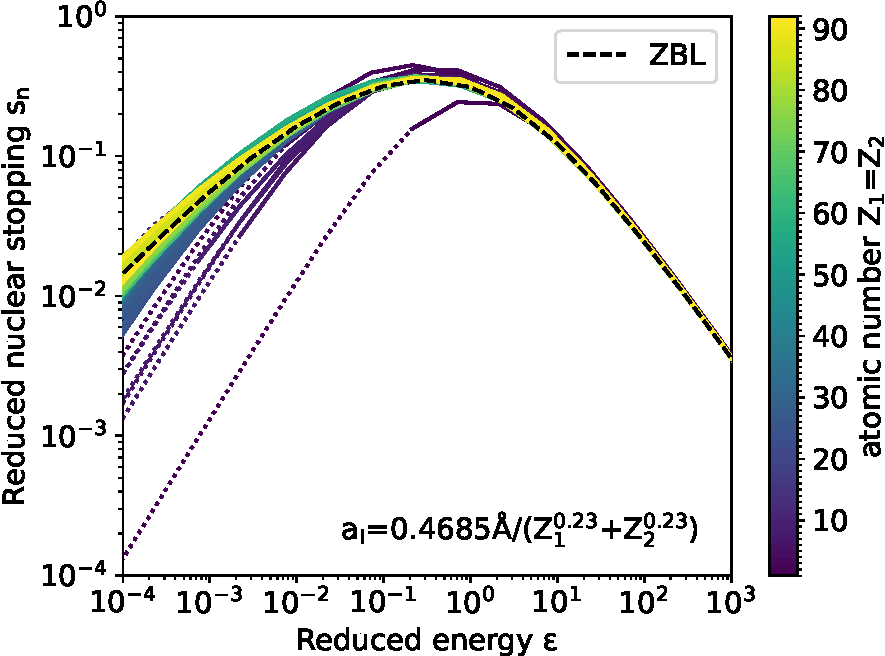
\includegraphics[scale=0.5]{sn_p0.23_p1_homo.pdf} ~~
    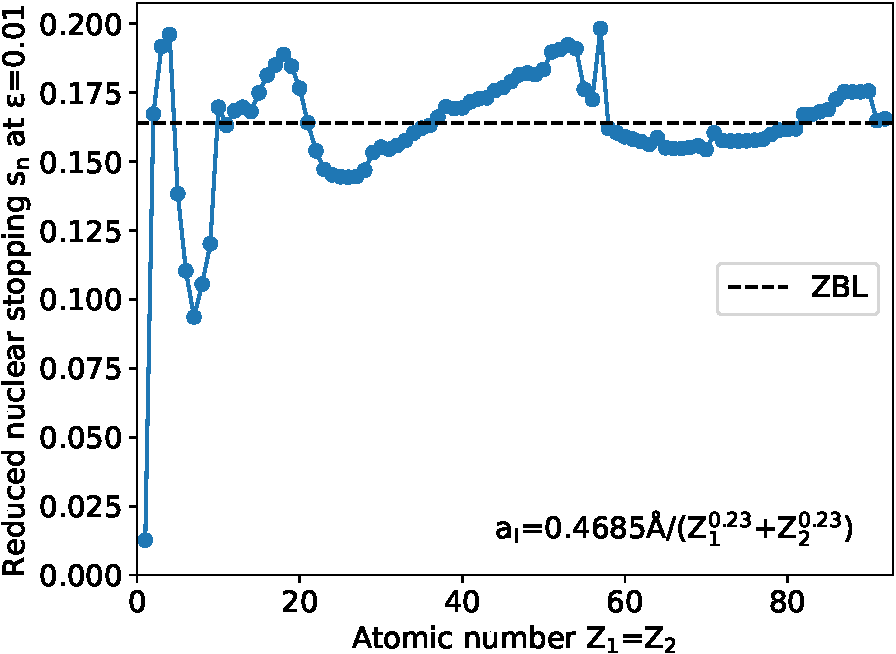
\includegraphics[scale=0.5]{sn_p0.23_p1_homo_e0.01.pdf} ~~ \\[\baselineskip]
    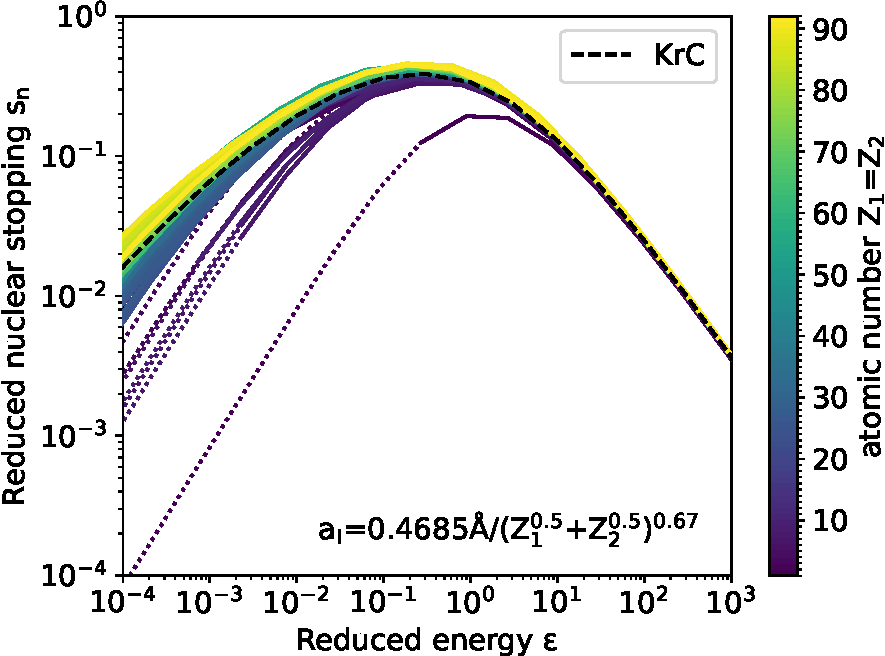
\includegraphics[scale=0.5]{sn_p0.5_p0.67_homo.pdf} ~~
    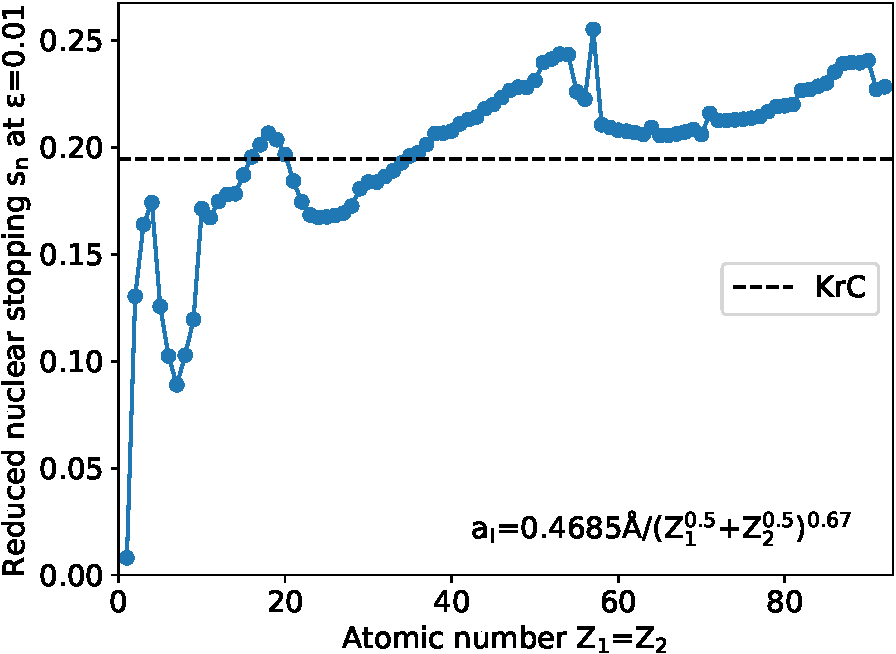
\includegraphics[scale=0.5]{sn_p0.5_p0.67_homo_e0.01.pdf}
    \caption{Reduced nuclear stopping cross section for the NLHlin potential (colored lines) of homonuclear atom pairs ($Z_1=Z_2$) as a function of reduced energy $\varepsilon$ (left) and for $\varepsilon = 0.01$ as a function of atomic number (right).
        Two different screening lengths have been used.
        Upper row: ZBL screening length \cref{eq:sn_aZBL}; lower row: Firsov screening length \cref{eq:sn_aF}
        For comparison, the stopping cross sections of the ZBL potential (upper row) and the KrC potential (lower row) are depicted by black dashed lines.
        Note that these two potentials yield universal reduced stopping cross sections with the respective screening lengths.
        In the left panels the atomic numbers are color-coded.
        The dotted parts of the lines correspond to energies $< 10$~eV.
    }
    \label{fig:sn_sn}
\end{figure}
%
The reduced nuclear stopping cross sections $S_\mathrm{n}$ for the NLHlin potentials are shown as a function of reduced energy $\varepsilon$ in \cref{fig:sn_sn} for homo-nuclear pairs.
Considerable variation is observed, in particular at low energies, which cannot be described by universal interatomic potentials like ZBL and KrC.
Comparing the results for the universal and the NLHlin potentials at $\varepsilon < 1$, the ZBL potential lies at the upper limit of the NLHlin potentials, while the KrC potential better approximates the average of the heavier elements ($Z \gtrsim 40$).
On the other hand, KrC does even worse than ZBL for the lighter elements ($Z \lesssim 20$), which is mainly due to the Firsov screening length (check!).

\begin{figure}
    \centering
    
\includegraphics[scale=0.5]{sn_ratio_homo_zbl_at_e.pdf} ~~
    
\includegraphics[scale=0.5]{sn_ratio_homo_krc_at_e.pdf}
    \caption{Ratio of the stopping cross section calculated using the NLHlin potential and the ZBL potential (left) or KrC potential (right) as a function of atomic number for four different energies. The data has been obtain for the homonuclear case ($Z_1 = Z_2$).}
    \label{fig:sn_sn_ratio}
\end{figure}
%
For the light ions the low values of the reduced energy are of no relevance since they correspond to energies where the BCA breaks down.
It is therefore more instructive to plot the nuclear stopping cross section as a function of the actual energy.
\cref{fig:sn_sn_ratio} shows the ratios of the stopping cross sections calculated using the NLHlin potential and the ZBL potential or KrC potential as a function of atomic number for four different energies for the homonuclear case ($Z_1 = Z_2$).
Compared to when the stopping cross section is plotted for constant reduced energies (\cref{fig:sn_sn}), the deviations from 1 appear more evenly distributed between light and heavy ions.

It is noted that in BCA simulations, impact parameters must be limited by some maximum value $p_\mathrm{max}$.
This value is often chosen relatively small, so that considerable energy loss is neglected at low energies (check!).
Thus, the effective stopping cross section is lowered in the simulation, possibly towards the values for the NLHlin potential, however, in an unsystematic way.

\begin{figure}
    \centering
    
\includegraphics[scale=0.5]{sn_zbl_all_e0.01.pdf} ~~
    
\includegraphics[scale=0.5]{sn_krc_all_e0.01.pdf}
    \caption{Reduced nuclear stopping cross section for the NLHlin potential of all atom pairs as a function of atomic number $Z_1$ at a reduced energy of $\varepsilon = 0.01$.
    Two different screening lengths have been used.
    Left: ZBL screening length \cref{eq:sn_aZBL}; right: Firsov screening length \cref{eq:sn_aF}
    For comparison, the stopping cross sections of the ZBL potential (left) and the KrC potential (right) are depicted by black dashed lines.
    Note that these two potentials yield universal reduced stopping cross sections with the respective screening lengths.
    The atomic numbers $Z_2$ are color-coded.
    }
    \label{fig:sn_sn_all}
\end{figure}
%
The stopping cross sections for all atom pairs at $\varepsilon = 0.02$ are depicted in \cref{fig:sn_sn_all}.
The results are in line with those for the homo-nuclear pairs (\cref{fig:sn_sn}).


\subsubsection{Nuclear straggling}
%%%%%%%%%%%%%%%%%%%%%%%%%%%%%%%%%%
%
It may be shown \cite{Bohr1948} that the variance of the energy loss due to nuclear collisions over a path length $\mathrm{d} r$ in a target with randomly positioned atoms is given by
%
\begin{equation}
    \label{eq:sn_sn_Estraggle}
    \overline{ \left( \mathrm{d} E - \overline{\mathrm{d} E} \right)^2 } =
        \int_0^\infty T_\mathrm{n}^2(E,p) \,
        2 \pi p \, \mathrm{d} p \, \mathrm{d} r N =
    N \mathrm{d} r \, Q_\mathrm{n}(E)
\end{equation}
%
with
%
\begin{equation}
    Q_\mathrm{n}(E) = \int_0^\infty T_\mathrm{n}^2(E,p) \, 2 \pi p \, \mathrm{d} p ~,
\end{equation}
%
which is usually called ``nuclear straggling''. Using \cref{eq:sn_sn_dE}, we obtain
%
\begin{equation}
    Q_\mathrm{n}(E) = \pi \gamma^2 E^2 \int_0^\infty \sin ^4 \frac{\theta}{2} \, 2 p \, \mathrm{d} p ~.
\end{equation}
%
In terms of the reduced quantities Eqs.~(\ref{eq:sn_reduced_lengths}) and (\ref{eq:sn_reduced_energy}) the nuclear straggling may also be written
%
\begin{equation}
    \label{eq:sn_qn1}
    Q_\mathrm{n}(E) = \pi \gamma^2 (E/\varepsilon)^2 a_\mathrm{I}^2 \, q_\mathrm{n}(\varepsilon)
\end{equation}
%
with
%
\begin{equation}
    q_\mathrm{n}(\varepsilon) = \varepsilon^2 \int_0^\infty \sin^4 \frac{\theta(\varepsilon,P)}{2} \, 2 P \, \mathrm{d} P ~.
\end{equation}
%
With Eqs.~(\ref{eq:sn_reduced_energy}) and (\ref{eq:sn_coulomb}), \cref{eq:sn_qn1} can be rewritten
%
\begin{equation}
    \label{eq:sn_qn}
    Q_\mathrm{n}(E) =  \pi \left[ \frac{ 4 M_1 }{ M_1 + M_2 }
        Z_1 Z_2 (14.4 \,\mathrm{eV\mathAA}) \right]^2 \, q_\mathrm{n}(\varepsilon) ~.
\end{equation}

The results for the nuclear straggling for the NLHlin potentials are shown in \cref{fig:sn_qn}.
They compare similarly to the ZBL and KrC potential as the nuclear stopping cross sections.
%
\begin{figure}
    \centering
    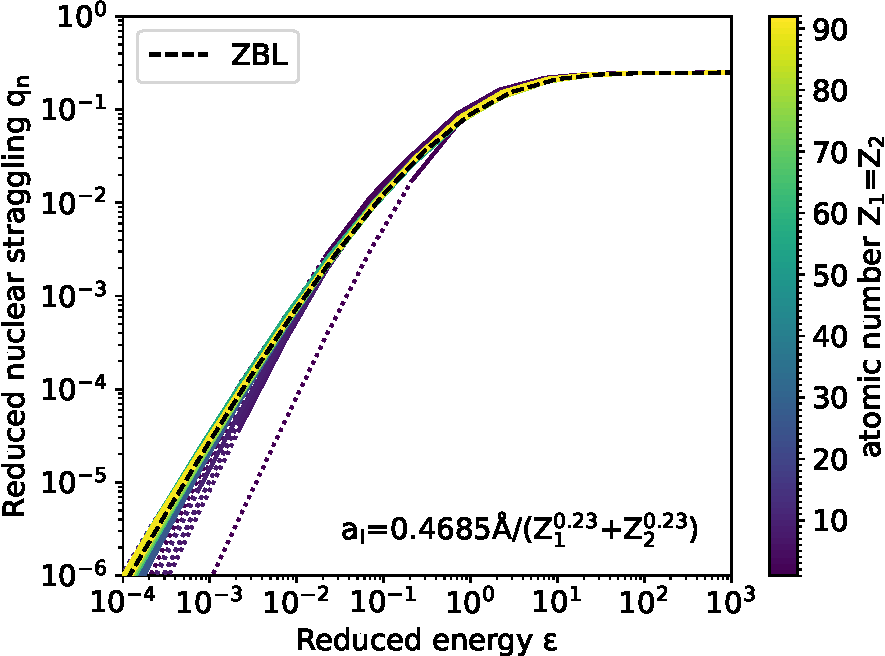
\includegraphics[scale=0.5]{qn_p0.23_p1_homo.pdf} ~~
    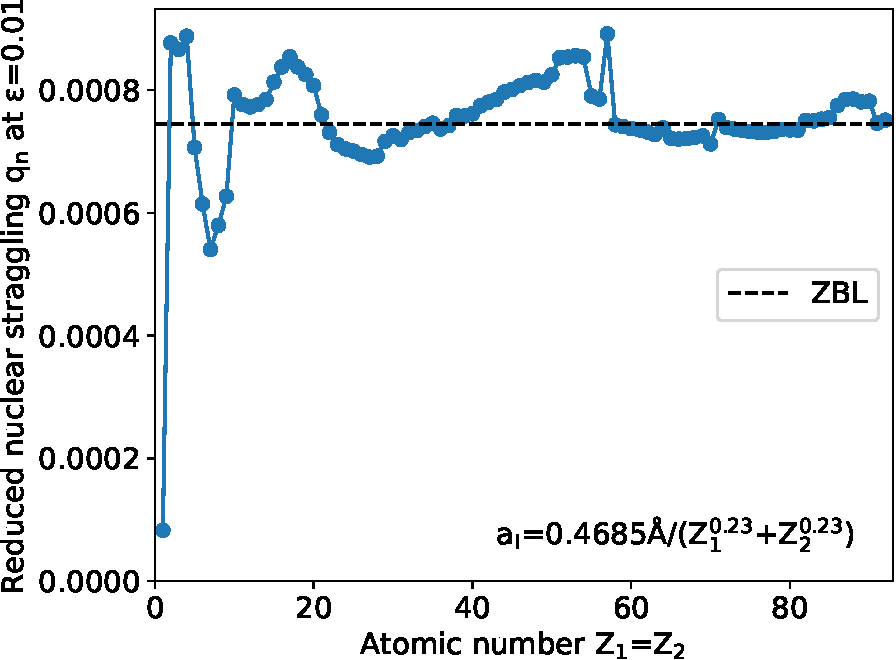
\includegraphics[scale=0.5]{qn_p0.23_p1_homo_e0.01.pdf} \\[\baselineskip]
    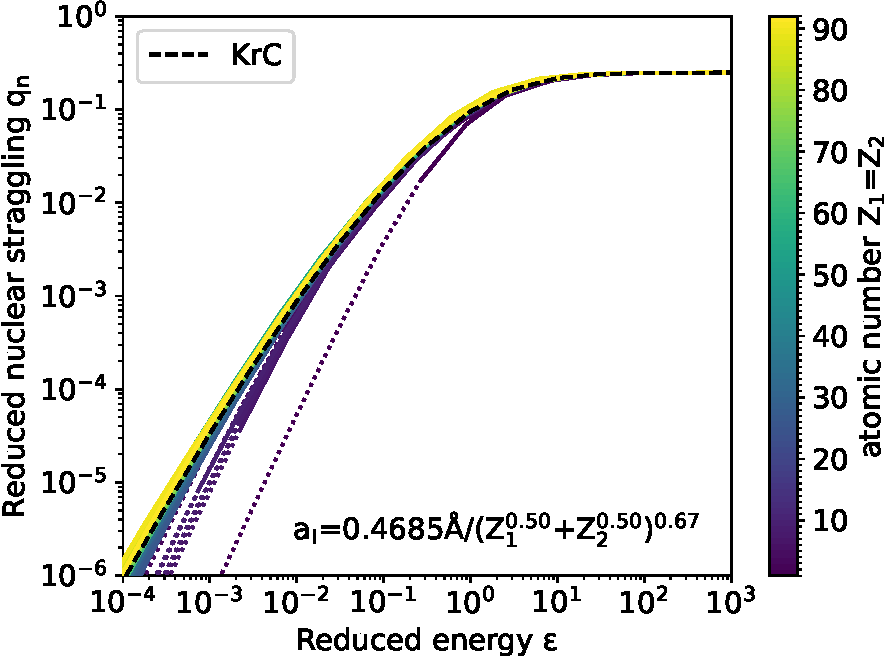
\includegraphics[scale=0.5]{qn_p0.5_p0.67_homo.pdf} ~~
    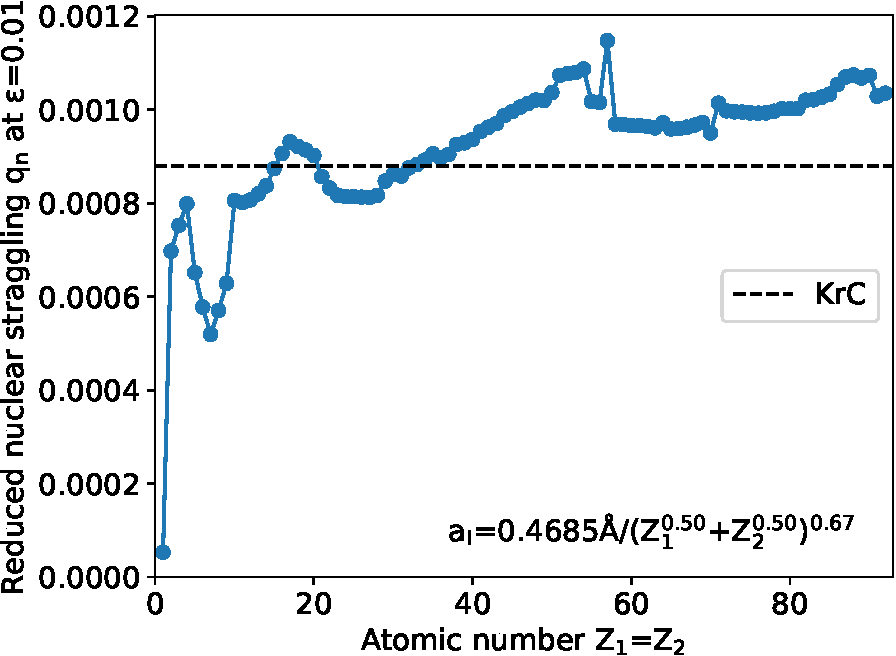
\includegraphics[scale=0.5]{qn_p0.5_p0.67_homo_e0.01.pdf}
    \caption{Reduced nuclear straggling for the NLHlin potential (colored lines) of homonuclear atom pairs ($Z_1=Z_2$) as a function of reduced energy $\varepsilon$ (left) and for $\varepsilon = 0.01$ as a function of atomic number (right).
    Two different screening lengths have been used.
    Upper row: ZBL screening length \cref{eq:sn_aZBL}; lower row: Firsov screening length \cref{eq:sn_aF}
    For comparison, the stopping cross sections of the ZBL potential (upper row) and the KrC potential (lower row) are depicted by black dashed lines.
    Note that these two potentials yield universal reduced stragglings with the respective screening lengths.
    In the left panels the atomic numbers are color-coded.
    The dotted parts of the lines correspond to energies $< 10$~eV.
    }
    \label{fig:sn_qn}
\end{figure}

\subsubsection{Analytic expressions}
%%%%%%%%%%%%%%%%%%%%%%%%%%%%%%%%%%%%
%
The results for the nuclear stopping cross section and straggling can be fitted by analytical expressions within a few percent as proposed in \cite{ZBL85}. For the stopping cross section we use
%
\begin{equation}
    \label{eq:sn_sn_fit}
    s_\mathrm{n}(\varepsilon) = \frac{ \ln(1 + a \, \varepsilon) }{
                          2 ( \varepsilon + b \, \varepsilon^c + d \, \varepsilon^{0.5})}
\end{equation}
%
In \cite{ZBL85} it is suggested to use $s_\mathrm{n} = \ln \varepsilon / 2 \varepsilon$ for $\varepsilon > 30$, which is referred to as ``unscreened nuclear stopping'' without further explanation.
We did not find it necessary to apply this special treatment for high energies, and found actually better fitting of the data using the expression \cref{eq:sn_sn_fit} over the whole energy range (at least) up to $\varepsilon = 10^4$.

For the nuclear straggling we use \cite{ZBL85}
%
\begin{equation}
    \label{eq:sn_qn_fit}
    q_\mathrm{n}(\varepsilon) = \frac{ 1 }{ 4 + a \, \varepsilon^b + c \, \varepsilon^d }
\end{equation}
%
The values $a$, $b$, $c$, and $d$ have been fitted to energies between $\varepsilon = 3 \times 10^{-5}$ and $10^4$ for both nuclear stopping cross section and nuclear straggling for all atom pairs.

\begin{figure}
    \centering
    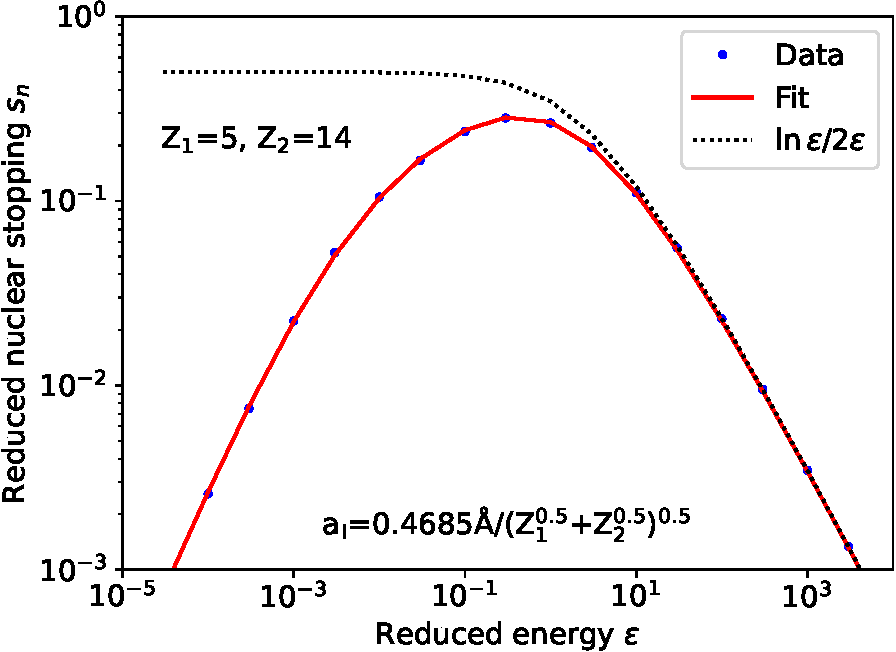
\includegraphics[scale=0.5]{sn_fit_nlhlin_B_Si.pdf} ~~
    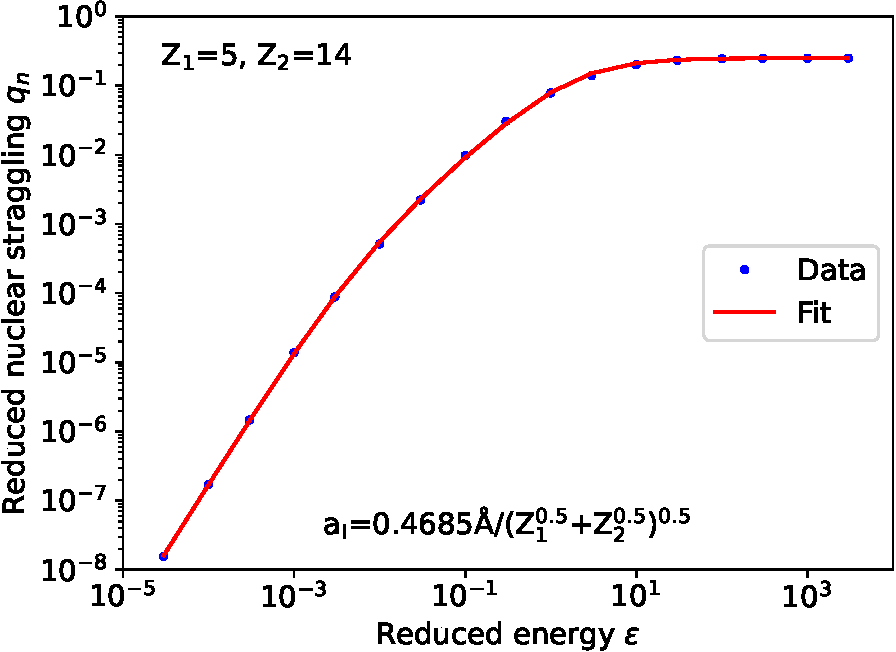
\includegraphics[scale=0.5]{qn_fit_nlhlin_B_Si.pdf}
    \caption{Data and fits for $Z_1 = 5$, $Z_2 = 14$.}
    \label{fig:sn_fit_Z5_14}
\end{figure}
%
\begin{figure}
    \centering
    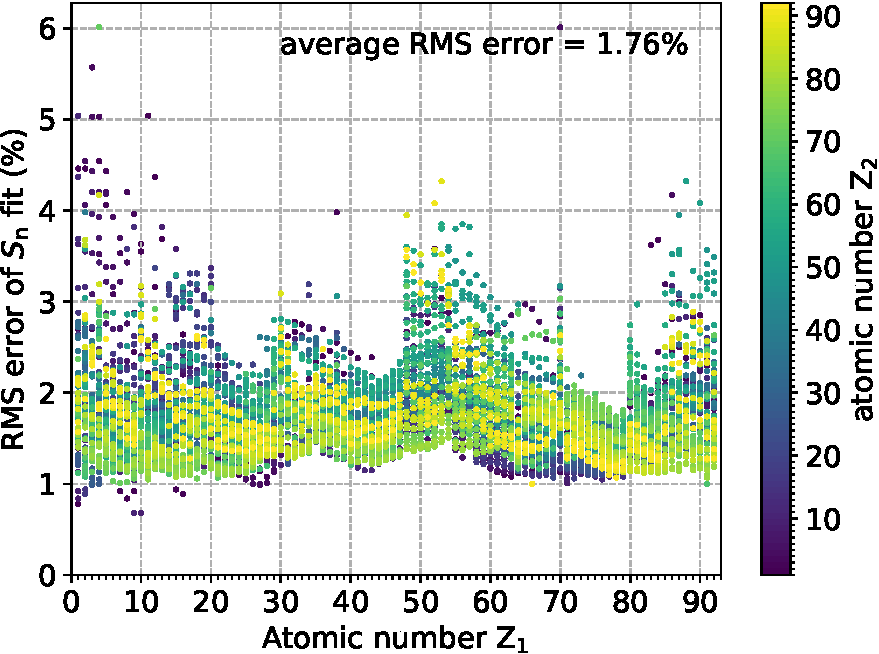
\includegraphics[scale=0.5]{sn_fit_error_nlhlin.pdf} ~~
    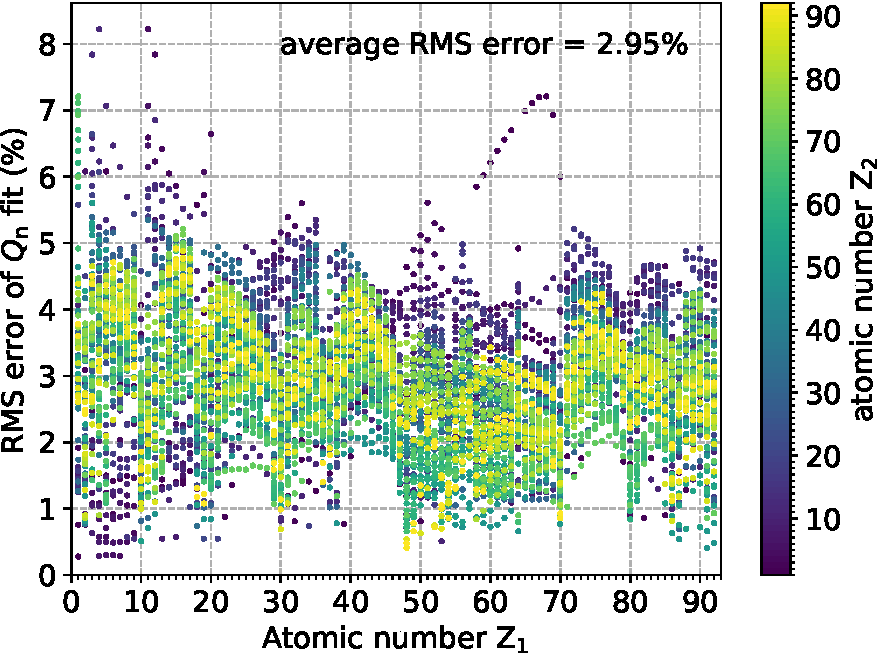
\includegraphics[scale=0.5]{qn_fit_error_nlhlin.pdf}
    \caption{Root-mean-square fit errors of the nuclear stopping cross section (left) and nuclear straggling (right) for all atom pairs.}
    \label{fig:sn_fit_error}
\end{figure}
%
\Cref{fig:sn_fit_Z5_14} shows, as an example the data and fits for $Z_1 = 5$, $Z_2 = 14$.
The root-mean-square fit errors for all atom pairs are shown in \cref{fig:sn_fit_error}.
Most of the fit errors is between 1 and 2.5\% for the nuclear stopping cross section and between 1.5 and 4\% for the nuclear straggling, with a mean of 1.76\% and 2.95\%,respectively, and a few errors up to 6\% and 8\%, respectively.

\section{Range}
\label{s:range}
The range of the ions is determined by both nuclear and electronic stopping. The average energy loss per path length is therefore given by
%
\begin{equation}
    \frac{ \mathrm{d} E' }{ \mathrm{d} r } =
        \left( \frac{ \mathrm{d} E' }{ \mathrm{d} r } \right)_\mathrm{n} +
        \left( \frac{ \mathrm{d} E' }{ \mathrm{d} r } \right)_\mathrm{e} =
        - N (S_\mathrm{n}(E') + S_\mathrm{e}(E'))
\end{equation}
%
where $S_\mathrm{e}$ characterizes the energy loss to electrons but is otherwise defined like $S_\mathrm{n}$. Compared to \cref{eq:sn_sndef}, we have replaced energy $E$ by $E'$ to distinguish the initial energy $E$ from the current energy $E'$. Separation of variables and integration of the path length from $0$ to $R$ and of energy from $E$ to $0$ gives the total path length
%
\begin{equation}
    \label{eq:sn_range}
    R = \int_0^E \frac{ \mathrm{d} E' }{ N (S_\mathrm{n}(E') + S_\mathrm{e}(E'))}
\end{equation}
%
In differential form this reads
%
\begin{equation}
    \label{eq:sn_range_differential}
    \frac{ \mathrm{d} R }{ \mathrm{d} E } =
        \frac{ 1 }{ N (S_\mathrm{n}(E) + S_\mathrm{e}(E))}
\end{equation}
%
We have silently neglected the statistical nature of nuclear stopping by dropping the overbar of \cref{eq:sn_sndef}. Lindhard \cite{Lin63} showed that $R$ is a satisfactory approximation of the mean range along the path.

Projected range is defined by the projection of the stop position of an ion to its initial direction, measured from its initial position. The distribution of projected ranges is what is measured when a depth profile is determined of ions implanted into a flat target at normal incidence, with its origin at the surface. The most basic characteristics of this distribution is the mean penetration depth or mean projected range $R_\mathrm{p}$, which in sloppy parlance is called ``the'' projected range.

It has been shown \cite{Bie82,Ash91}, that an approximation to the projected range can be calculated from
%
\begin{equation}
    \label{eq:sn_rp_differential}
    \frac{ \mathrm{d} R_\mathrm{p} }{ \mathrm{d} E } =
        \frac{ 1 }{ N (S_\mathrm{n}(E) + S_\mathrm{e}(E))}
        \left( 1 - \frac{ \mu N S_\mathrm{n} }{ 2 E } R_\mathrm{p} \right),
        \quad \mu = \frac{ M_2 }{ M_1 }
\end{equation}

\begin{figure}
    \centering
    
\includegraphics[scale=0.5]{rp_As_Si.pdf}
    \caption{Projected range $R_\mathrm{p}$ as a function of energy for the NLHlin potential (solid line) and the ZBL potential (dashed and dotted lines). For the ZBL potential, our own results (dotted line) agree well with those obtained by SRIM \cite{SRIM-2013}.}
    \label{fig:sn_rp_As_Si}
\end{figure}
%
\begin{figure}
    \centering
    
\includegraphics[scale=0.5]{rp_ratio_homo_zbl.pdf} ~~
    
\includegraphics[scale=0.5]{rp_ratio_homo_zbl_at_e}
    \caption{The ratio of the projected ranges calculated with the NLHlin and ZBL potentials as a function of energy (left) and as a function of atomic number (right) for homonuclear atom pairs.}
    \label{fig:sn_rp_ratio_homo_zbl}
\end{figure}
%
\begin{figure}
    \centering
    
\includegraphics[scale=0.5]{rp_ratio_homo_krc.pdf} ~~
    
\includegraphics[scale=0.5]{rp_ratio_homo_krc_at_e}
    \caption{The ratio of the projected ranges calculated with the NLHlin and KrC potentials as a function of energy (left) and as a function of atomic number (right) for homonuclear atom pairs.}
    \label{fig:sn_rp_ratio_homo_krc}
\end{figure}
%
Using tabulated $S_\mathrm{e}$ values from SRIM \cite{SRIM-2013}, the projected ranges have been calculated as a function of energy.
Results for As in Si are shown in \cref{fig:sn_rp_As_Si}.
The ratios of the projected ranges obtained with the NLHlin potentials and the ZBL potential are shown in \cref{fig:sn_rp_ratio_homo_zbl} as a function of implantation energy.
The ratios of the projected ranges obtained with NLHlin and KrC potential is depicted in \cref{fig:sn_rp_ratio_homo_krc}.
Very significant deviations between the NLHlin and the conventional potentials can be seen except for the noble gases ($Z=2,10,18,36,54,86$).
Comparing Figs.~\ref{fig:sn_rp_ratio_homo_zbl} and \ref{fig:sn_rp_ratio_homo_krc}, KrC performs much better than ZBL for heavy atoms, while KrC performs poorer for lighter elements.

\begin{figure}
    \centering
    
\includegraphics[scale=0.5]{rp_ratio_all_zbl_at_e.pdf} ~~
    
\includegraphics[scale=0.5]{rp_ratio_all_krc_at_e.pdf}
    \caption{Projected range ratio with respect to ZBL (left) and KrC (right) for all combinations of $Z_1$ and $Z_2$.}
    \label{fig:sn_ratio_all}
\end{figure}

\newpage
\begin{subappendices}
    \section{Gauss-Legendre Quadrature}
    \label{s:gauss-legendre}
    % Gauss-Legendre Quadrature

Gauss-Legendre quadrature approximates the integral
%
\begin{equation}
    \label{eq:sn_legendre_formula}
    \int_{-1}^1 h(u) \, \mathrm{d}u \approx \sum_{i=1}^n w_i h(u_i)
\end{equation}
%
where the abscissas \(u_i\) are the roots of the Legendre polynomial \(P_n(u)\) and the weights \(w_i\) are given by \cite[25.4.29]{Abr72}
%
\begin{equation}
    \label{eq:sn_legendre_weights}
    w_i = \frac{ 2 }{ (1-u_i^2) [P_n'(u_i)]^2 }
\end{equation}
%
The roots and abscissas are usually not calculated but taken from tabulated values, e.g. \cite{Hol10a}.

Adjustment of the integration boundaries may be achieved by a linear transformation of the integration variable:
%
\begin{equation*}
    \int_a^b h(u) \, \mathrm{d}u =
        \frac{ b-a }{ 2 } \int_{-1}^1 h \left( \frac{ (b-a) u + (b+a) }{ 2 } \right)
        \, \mathrm{d}u \approx
        \sum_{i=1}^n \tilde{w}_i \, h \left( \tilde{u} \right)
\end{equation*}
%
with
%
\begin{equation}
    \label{eq:sn_legendre_transform}
    \tilde{u}_i = \frac{ (b-a) u_i + (b+a) }{ 2 } , \qquad
        \tilde{w}_i = \frac{ b-a }{ 2 } w_i ~.
\end{equation}
%
Gauss-Legendre quadrature integrates polynomials of order \(< 2n\) exactly, so it is most accurate if all derivatives up to order \(2n-1\) exist and higher derivatives are small.


    \section{Impulse approximation}
    \label{sn:impulse}
    For high enough energies $E$ or small enough scattering angles, it may be assumed that the incoming projectile moves on a straight line at constant velocity.
To apply this approximation, a few notes on the center-of-mass system are necessary.
The transformation of the two-body system into the center-of-mass system, whose origin is in the center of mass of the projectile (atom 1) and the recoil (atom 2),
%
\begin{equation}
    \label{eq:sn_center-of-mass}
    \vec{x}_\mathrm{c} = \frac{m_1}{m_1+m_2} \vec{x}_1 + \frac{m_2}{m_1+m_2} \vec{x}_2 \, ,
\end{equation}
%
can be described in terms of the vector from recoil to projectile
%
\begin{equation}
    \label{eq:sn_vector_21}
    \vec{x}_\mathrm{r} = \vec{x}_1 - \vec{x}_2 \, .
\end{equation}
%
The time evolution of $\vec{x}_\mathrm{r}$ is the same as that of the position of a single particle with the (so-called) reduced mass
%
\begin{equation}
    \label{eq:sn_reduced_mass}
    m_\mathrm{r} = \frac{m_1 m_2}{m_1 + m_2} \, .
\end{equation}
%
in a stationary potential $V(\vec{x}_\mathrm{r})$.
The (constant) energy of the one-particle system with the reduced mass $m_\mathrm{r}$ equals the sum of the energies of the two particles with masses $m_1$ and $m_2$ in the center-of-mass system. Its value is
%
\begin{equation}
    \label{eq:sn_reduced_energy1}
    E_\mathrm{r} = \frac{ m_\mathrm{r} v_0^2}{ 2 }
\end{equation}
%
where $v_0$ is the velocity of the projectile in the laboratory system before the collision.
Note that it equals the velocity $\dot{\vec{x}}_\mathrm{r} = \dot{\vec{x}}_1 - \dot{\vec{x}}_2$ of the particle in the one-particles system, since before the collision $\dot{\vec{x}}_2 = 0$ and the potential energy is zero.
With the energy in the laboratory system $E = m_1 v_0^2/2$, we regain \cref{eq:sn_physics_Ec}:
%
\begin{equation*}
    E_\mathrm{c} = \frac{M_2}{M_1 + M_2} \, E .
\end{equation*}

Now assume that a projectile with mass $m_\mathrm{r}$ moves at constant speed $v_\mathrm{x} = v_0$ parallel to the $x$ axis at $y = p$ in a potential $V(r)$ centered at the origin. Its momentum is zero initially. During passage, the projectile receives an impulse (change in momentum) of
%
\begin{equation}
    \label{eq:sn_impulse_Fy}
    m_\mathrm{r} (v_\mathrm{y} - 0)
        = \int_{-\infty}^{\infty} F_\mathrm{y}(t) \, \mathrm{d}t
        = \frac{1}{v_\mathrm{x}}\int_{-\infty}^{\infty} F_\mathrm{y}(x) \, \mathrm{d}x
\end{equation}
%
where $v_\mathrm{y}$ denotes the $y$ component of the velocity after the collision and $F_\mathrm{y}$ the $y$ component of the force.
The scattering angle in the center-of-mass system is given by
%
\begin{equation}
    \label{eq:sn_theta_impulse_Fy}
    \theta \approx \tan \theta = \frac{v_\mathrm{y}}{v_\mathrm{x}}
    = \frac{1}{2 E_\mathrm{c}} \int_{-\infty}^{\infty} F_\mathrm{y}(x) \, \mathrm{d}x
    = \frac{1}{2 E} \frac{M_1+M_2}{M_2} \int_{-\infty}^{\infty} F_\mathrm{y}(x) \, \mathrm{d}x
\end{equation}
%
where we have used $E_\mathrm{c} = m_\mathrm{r} v_\mathrm{x}^2 / 2$ and \cref{eq:sn_physics_Ec}.
According to Eqs.~(\ref{eq:sn_physics_psi}) and (\ref{eq:sn_physics_dE}), the scattering angle in the laboratory system and the energy transfer are given by
%
\begin{equation}
    \label{eq:sn_impulse_psi_Fy}
    \psi_1 \approx \tan \psi_1 \approx \frac{M_2}{M_1 + M_2} \, \theta
    \approx \frac{1}{E} \left(
        \frac{1}{2} \int_{-\infty}^{\infty} F_\mathrm{y}(x) \, \mathrm{d}x
    \right)
\end{equation}
%
and
%
\begin{equation}
    \label{eq:sn_impulse_dE_Fy}
    \Delta E \approx \frac{M_1 M_2}{(M_1 + M_2)^2} \, E \, \theta^2
    \approx \frac{1}{E} \, \frac{M_1}{M_2} \left(
        \frac{1}{2} \int_{-\infty}^{\infty} F_\mathrm{y}(x) \, \mathrm{d}x
    \right)^2  ,
\end{equation}
%
respectively.
Like $\theta$, $\psi_1$ and $\Delta E$ are proportional to $1/E$.
Interestingly, $\psi_1$ does not depend on the atom masses $M_1$ and $M_2$.

For a spherically symmetric potential $V(r)$, the force in $y$ direction is given by
%
\begin{equation}
    \label{eq:sn_Fy}
    F_\mathrm{y}(x) = - \frac{\mathrm{d} V(r)}{\mathrm{d} r} \frac{p}{r}
        = - \frac{\mathrm{d} V(r)}{\mathrm{d} p}
\end{equation}
%
with
%
\begin{equation}
    \label{eq_sn_r_from_x}
    r = \sqrt{x^2 + p^2} .
\end{equation}
%
The first expression after the equal sign in \cref{eq:sn_Fy} takes the $y$ component of the force, which points in the direction of the vector from the origin to the projectile.
The second expression can be shown to be equivalent to the first one by applying the chain rule of differentiation.
Using either expression and making use of $\int_{-\infty}^0 = \int_0^\infty$, we obtain
%
\begin{equation}
    \label{eq:sn_impulse_V}
    \frac{1}{2} \int_{-\infty}^{\infty} F_\mathrm{y}(x) \, \mathrm{d}x
    = - \int_{0}^{\infty} \frac{\mathrm{d} V(r)}{\mathrm{d} r}
        \frac{p}{r} \, \mathrm{d}x
    = - \frac{\mathrm{d}}{\mathrm{d} p} \int_{0}^{\infty} V(r)
        \, \mathrm{d}x
\end{equation}
%
where in the second expression we have also changed the order of integration and differentiation.

If we further assume a screened Coulomb potential, \cref{eq:sn_screened_coulomb}, we obtain
%
\begin{equation}
    \label{eq:sn_impulse_Phi_r}
    \frac{1}{2} \int_{-\infty}^{\infty} F_\mathrm{y}(x) \, \mathrm{d}x
    = Z_1 Z_2 e^2
        \int_{0}^{\infty} \frac{\Phi(r) - r \, \Phi'(r)}{r^3} p
        \, \mathrm{d}x
    = - Z_1 Z_2 e^2 \, \frac{\mathrm{d}}{\mathrm{d} p} \int_{0}^{\infty} \frac{\Phi(r)}{r}
    \, \mathrm{d}x
\end{equation}
%
Using reduced lengths, \cref{eq:sn_reduced_lengths} and $X = x/a_\mathrm{I}$, \cref{eq:sn_impulse_Phi_r} can be rewritten as
%
\begin{equation}
    \label{eq:sn_impulse_P}
    \frac{1}{2} \int_{-\infty}^{\infty} F_\mathrm{y}(x) \, \mathrm{d}x
    = \frac{Z_1 Z_2 e^2}{a_\mathrm{I}} \, I(P)
\end{equation}
%
with the dimensionless integral
%
\begin{equation}
    \label{eq:sn_impulse_Phi_R}
    I(P)
    = \int_{0}^{\infty} \frac{\Phi(R) - R \, \Phi'(R)}{R^3} P \, \mathrm{d}X
    = - \frac{\mathrm{d}}{\mathrm{d} P} \int_{0}^{\infty} \frac{\Phi(R)}{R}
        \, \mathrm{d}X .
\end{equation}
%
Inserting \cref{eq:sn_impulse_P} in Eqs.~(\ref{eq:sn_impulse_psi_Fy}) and (\ref{eq:sn_impulse_dE_Fy}), we obtain
%
\begin{equation}
    \label{eq:sn_impulse_psi_I}
    \psi_1 \approx \frac{Z_1 Z_2 e^2}{a_\mathrm{I}} \, \frac{I(P)}{E}
\end{equation}
%
and
%
\begin{equation}
    \label{eq:sn_impulse_dE_I}
    \Delta E \approx  \frac{M_1}{M_2} \left(
        \frac{Z_1 Z_2 e^2}{a_\mathrm{I}}
    \right) ^2
    \frac{I(P)^2}{E} .
\end{equation}

The second expression on the right-hand side of \cref{eq:sn_impulse_Phi_R} is favorable for infinite range sum-of-exponentials screening functions, \cref{eq:sn_sum_exp}. Using the transformation $t = R/P = \sqrt{1 + X^2/P^2}$, the integrals evaluate to \cite[8.432.3]{Gra80}
%
\begin{equation*}
    \int_0^\infty \frac{\exp(-b_i R)}{R} \, \mathrm{d}X
    = \int_{1}^{\infty} \frac{\exp (-b_i P t)}{\sqrt{t^2 - 1}} \, \mathrm{d}t
    = K_0(b_i P)
\end{equation*}
%
where $K_0(x)$ is the modified Bessel function of second kind and order 0. $I(P)$ therefore evaluates to
%
\begin{equation}
    I(P) = - \sum_i a_i \frac{\mathrm{d} K_0(b_i P)}{\mathrm{d} P}
    = \sum_i a_i b_i K_1(b_i P)
\end{equation}
%
where $K_1(x)$ is the modified Bessel function of second kind and order 1.
For other screening functions, the first integral on the right-hand side of \cref{eq:sn_impulse_Phi_R} is preferable, since it does not require numerical differentiation.

\subsubsection{Selection of the maximum impact parameter}
%%%%%%%%%%%%%%%%%%%%%%%%%%%%%%%%%%%%%%%%%%%%%%%%%%%%%%%%%
The impulse approximation can be used to estimated the maximum impact parameter that is necessary to to consider all collisions with scattering angles and energy transfers about some chosen limit.
This is because the desired limit of the scattering angle usually is quite low, say $\sim 1\degree$.

With a purely repulsive interatomic potential, increasing impact parameters $P$ result in decreasing scattering angles $\psi_1$, so according to \cref{eq:sn_impulse_psi_I}, $I(P)$ should be a monotonically decreasing function.%
%
\footnote{This could be violated when the impulse approximation fails.}
%
Then, according to \cref{eq:sn_impulse_dE_I}, also $\Delta E(P)$ is monotonically decreasing.
Thus, if we want to guarantee that by choosing the impact parameter between $0$ and $P_\mathrm{max}$ we do not miss any collisions with either $\psi_1 > \psi_\mathrm{min}$ or $\Delta E > \Delta E_\mathrm{min}$, both $\psi_1(P_\mathrm{max}) \le \psi_\mathrm{min}$ and $\Delta E(P_\mathrm{max}) \le \Delta E_\mathrm{min}$ must hold.
The minimum $P_\mathrm{max}$ for which both conditions are met is the one where the ``$\le$'' sign is replaced by the ``$=$'' sign in one of the conditions, whatever occurs first when $P_\mathrm{max}$ is decreased.

As can be seen from Eqs.~(\ref{eq:sn_impulse_psi_I}) and (\ref{eq:sn_impulse_dE_I}), the resulting conditions for $P_\mathrm{max}$ depend on the projectile energy $E$.
On the other hand, for a given $P_\mathrm{max}$, conditions for $E$ result from $\psi_1(P_\mathrm{max}) \le \psi_\mathrm{min}$ and $\Delta E(P_\mathrm{max}) \le \Delta E_\mathrm{min}$:
%
\begin{equation}
    \label{eq:sn_cond_e_psimin}
    E \ge \frac{Z_1 Z_2 e^2}{a_\mathrm{I}}
        \frac{I(P_\mathrm{max})}{\psi_\mathrm{min}}
\end{equation}
%
\begin{equation}
    \label{eq:sn_cond_e_dEmin}
    E \ge \frac{M_1}{M_2} \left( \frac{Z_1 Z_2 e^2}{a_\mathrm{I}} \right) ^2
        \frac{I(P_\mathrm{max})^2}{\Delta E_\mathrm{min}} \, .
\end{equation}
%
from $\Delta E(P_\mathrm{max}) \le \Delta E_\mathrm{min}$.
Since both conditions must be met, $E$ must be larger than or equal to the larger one of the two right-hand sides of Eqs.~(\ref{eq:sn_cond_e_psimin}) and (\ref{eq:sn_cond_e_dEmin}).
If we now denote as $P_\mathrm{max}$ the \textbf{smallest value of the maximum impact parameter that fulfills the conditions}, we have to replace the ``$\ge$'' sign by the ``$=$'' sign:
%
\begin{equation}
    \label{eq:sn_varepsilon_pmaxmin}
    E = \max \left(
        \frac{Z_1 Z_2 e^2}{a_\mathrm{I}}
        \frac{I(P_\mathrm{max})}{\psi_\mathrm{min}},
        \frac{M_1}{M_2} \left( \frac{Z_1 Z_2 e^2}{a_\mathrm{I}} \right) ^2
        \frac{I(P_\mathrm{max})^2}{\Delta E_\mathrm{min}} .
    \right) .
\end{equation}
%
\cref{eq:sn_varepsilon_pmaxmin} can be used to generate a table of $P_\mathrm{max}$-$E$ pairs, which can then be used to interpolate $P_\mathrm{max}$ values for given energies $E$.

\begin{figure}
    \centering
    
\includegraphics[scale=0.5]{impulse_nlhlin_He_W.pdf} ~~
    
\includegraphics[scale=0.5]{impulse_nlhlin_As_Si.pdf}
    \caption{Determination of the maximum impact parameter from minimum scattering angle and energy transfer.
    Left: 3 keV He in W, using the surface binding energy of W (8.68 eV) as the minimum energy transfer and 3\textdegree\ as the minimum scattering angle.
    Right: 100 keV As in Si, using the threshold displacement energy of Si (15 eV) as the minimum energy transfer and 1\textdegree\ as the minimum scattering angle.}
    \label{fig:sn_impulse}
\end{figure}
%
The selection of the maximum impact parameter is illustrated in \cref{fig:sn_impulse} with two examples.
In the first example, W is bombarded with He at 3~keV. One is interested in sputtering, therefore the surface binding energy is used in the energy criterion.
Moderately accurate trajectories are desired, so the minimum scattering angle is chosen as 3\textdegree.
The two choices correspond to two maximum impact parameters.
The larger one, resulting from the desired minimum scattering angle, has to be selected, since both conditions must be fulfilled.
In the other example shown in \cref{fig:sn_impulse}, Si is bombarded with 100~keV As.
Here one wishes to include all damage generation events in the simulation, so a minimum energy transfer equal to the threshold displacement energy is chosen.
Accurate trajectories are warranted by a small minimum scattering angle of 1\textdegree.
Again, the larger one of the two resulting maximum impact parameters must be chosen.

Note that the impulse approximation always yields upper limits to the energy transfer and scattering angle.
Their graphs as a function of impact parameter therefore are always to the right of the exact values (dashed vs.\ solid lines in \cref{fig:sn_impulse}).
The estimate of the maximum impact parameter therefore is an upper limit to what the exact calculation would yield.
This means, using the maximum impact parameter so determined, one might occasionally include events with energy transfers or scattering angles below the chosen limits, but one would not omit events above these limits.

    \section{Alternative Calculation of the Apsis of Collision}
    \label{s:apsis_alt}
    \subsubsection{Obtaining an initial condition}
%%%%%%%%%%%%%%%%%%%%%%%%%%%%%%%%%%%%%%%%%%%%%%
%
An alternative approach to finding an initial solution of \cref{eq:sn_apsis_eq},
%
\begin{equation}
    \label{eq:sn_apsis_alt_eq}
    f(R) = R - \frac{1}{\varepsilon} \Phi(R) - \frac{P^2}{R} = 0.
\end{equation}
%
is to approximate $\Phi(R)$ by a piecewise function $\phi(R)$ which is always larger than or equal to $\Phi(R)$, and which allows \cref{eq:sn_apsis_alt_eq}.
Such a function is
%
\begin{equation}
    \label{eq:sn_apsis_alt_approx}
    \phi(R) =
        \begin{cases}
            1 - k_1 R                 &  \text{for $0 \le R \le R_{12}$} \\
            k_2 / R                   &  \text{for $R_{12} \le R \le R_{23}$} \\
            k_3 / R^3                 &  \text{for $R_{23} \le R \le R_{34}$} \\
            k_4 (R_\mathrm{max} - R)  &  \text{for $R_{34} \le R$} \\
        \end{cases}
\end{equation}
%
where the last case is used only with a finite maximum range $R_\mathrm{max}$, and $R_{12}$, $R_{23}$, and $R_{34}$ are chosen such that the function is continuous and its first derivative is continuous at $R_{12}$ and $R_{34}$:
%
\begin{equation}
    \label{eq:sn_apsis_alt_join}
    k_1 = \frac{ 1 }{ 4 k_2 },
    \quad R_{12} = \sqrt{ \frac{ k_2 }{ k_1 }},
    \quad R_{23} = \sqrt{ \frac{ k_3 }{ k_2 }},
    \quad R_{34} = \frac{3}{4} R_\mathrm{max},
    \quad k_4 = \frac{ 3 k_3 }{ R_{34}^4 }
\end{equation}
%
The constants $k_2$ and $k_3$ are chosen such that the function touches $\Phi(R)$, i.e., $\phi(R) = \Phi(R)$ and $\phi'(R) = \Phi'(R)$.
The touch points and coefficients are obtained by solving the equations
%
\begin{equation}
    \Phi(R_2) + R_2 \Phi'(R_2) = 0, \qquad k_2 = R_2 \Phi(R_2)
\end{equation}
%
and
%
\begin{equation}
    \Phi(R_3) + \frac{1}{3} R_3 \Phi'(R_3) = 0, \qquad k_3 = R_3^3 \Phi(R_3)
\end{equation}

In order to approximately solve \cref{eq:sn_apsis_alt_eq}, we replace $\Phi(R)$ by $\phi(R)$ for each of the three intervals and obtain
%
\begin{equation}
    \label{eq:sn_apsis_alt_sol_R_tmp}
    R_0^{(0)} =
        \begin{cases}
            \displaystyle
            \frac{ 1 + \sqrt{ 1 + 4 (\varepsilon + k_1 ) \varepsilon P^2 }}{
                2 (\varepsilon + k_1 )}
            & \text{for } 0 \le R \le R_{12} \\[10pt]
            \sqrt{ P^2 + \frac{ k_2 }{ \varepsilon} }
            & \text{for } R_{12} \le R \le R_{23} \\[10pt]
            \sqrt{ \frac{ P^2 }{ 2 } + \sqrt{ \frac{ P^4 }{ 4 } + \frac{ k_3 }{ \varepsilon }}}
            & \text{for } R_{23} \le R \le R_{34} \\[10pt]
            \displaystyle
            \frac{ k_4 R_\mathrm{max}
                   + \sqrt{ (k_4 R_\mathrm{max})^2
                             + 4 (\varepsilon + k_4 ) \varepsilon P^2 }}{
            2 (\varepsilon + k_4 )}
            &  \text{for } R_{34} \le R \\
        \end{cases}
\end{equation}
%
Inserting the solutions $R_0^{(0)}$ into the conditions for $R$ and using \cref{eq:sn_apsis_alt_join}, one can rewrite the conditions in terms of $P^2 + k_2 / \varepsilon$, so that we finally obtain
\begin{equation}
    \label{eq:sn_apsis_alt_sol_R}
    R_0^{(0)} =
    \begin{cases}
        \displaystyle
        \frac{ 1 + \sqrt{ 1 + 4 (\varepsilon + k_1 ) \varepsilon P^2 }}{
            2 (\varepsilon + k_1 )}
        & \text{for } P^2 \le \frac{ k_2 }{ k_1 } - \frac{ k_2 }{ \varepsilon } \\[10pt]
        \sqrt{ P^2 + \frac{ k_2 }{ \varepsilon} }
        & \text{for } \frac{ k_2 }{ k_1 } - \frac{ k_2 }{ \varepsilon } \le P^2
            \le \frac{ k_3 }{ k_2 } - \frac{ k_2 }{ \varepsilon } \\[10pt]
        \sqrt{ \frac{ P^2 }{ 2 } + \sqrt{ \frac{ P^4 }{ 4 } + \frac{ k_3 }{ \varepsilon }}}
        & \text{for } \frac{ k_3 }{ k_2 } - \frac{ k_2 }{ \varepsilon } \le P^2
            \le R_{34}^2 - \frac{ k_3 }{ \varepsilon R_{34}^2 }\\[10pt]
            \displaystyle
        \frac{ k_4 R_\mathrm{max}
               + \sqrt{ (k_4 R_\mathrm{max})^2
                        + 4 (\varepsilon + k_4 ) \varepsilon P^2 } }{
               2 (\varepsilon + k_4 )}
        &  \text{for } R_{34}^2 - \frac{ k_3 }{ \varepsilon R_{34}^2 } \le P^2 \\
    \end{cases}
\end{equation}

The case $r > R_{34}$ cannot be used for screening functions with infinite range.
Instead, the procedure implemented in TRIM85 \cite{ZBL85} can be used, which solves the equation \cref{eq:sn_apsis_alt_eq} for the head-on case ($P=0$) for an approximate screening function $\Phi(R) = \exp(-0.37 R)$ by fix-point iteration:
%
\begin{equation}
    R = \frac{1}{\varepsilon} \exp(-0.37 R)
\end{equation}
%
Starting with $R = P$, up to two iterations are done, and the algorithm falls back to $R = P$ if $R$ gets smaller than $P$ during iteration.
If the approximation to the apsis determined in this way is smaller than the touch point of $k_3/R^3$, the remaining cases of \cref{eq:sn_apsis_alt_sol_R} can be used.

\subsubsection{Convergence}
%%%%%%%%%%%%%%%%%%%%%%%%%%%
%
\begin{figure}[htbp]
    \centering
    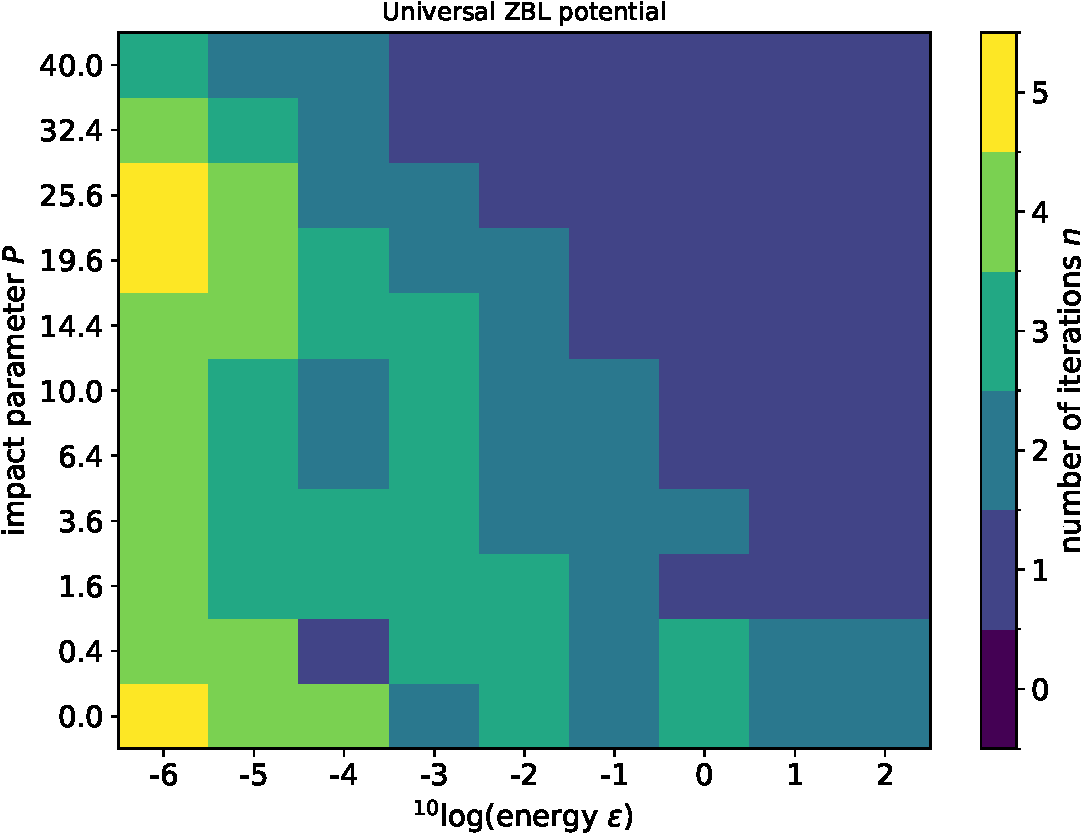
\includegraphics[scale=0.41]{ZBLuniv_iter_apsis_phiapprox.pdf} ~~
    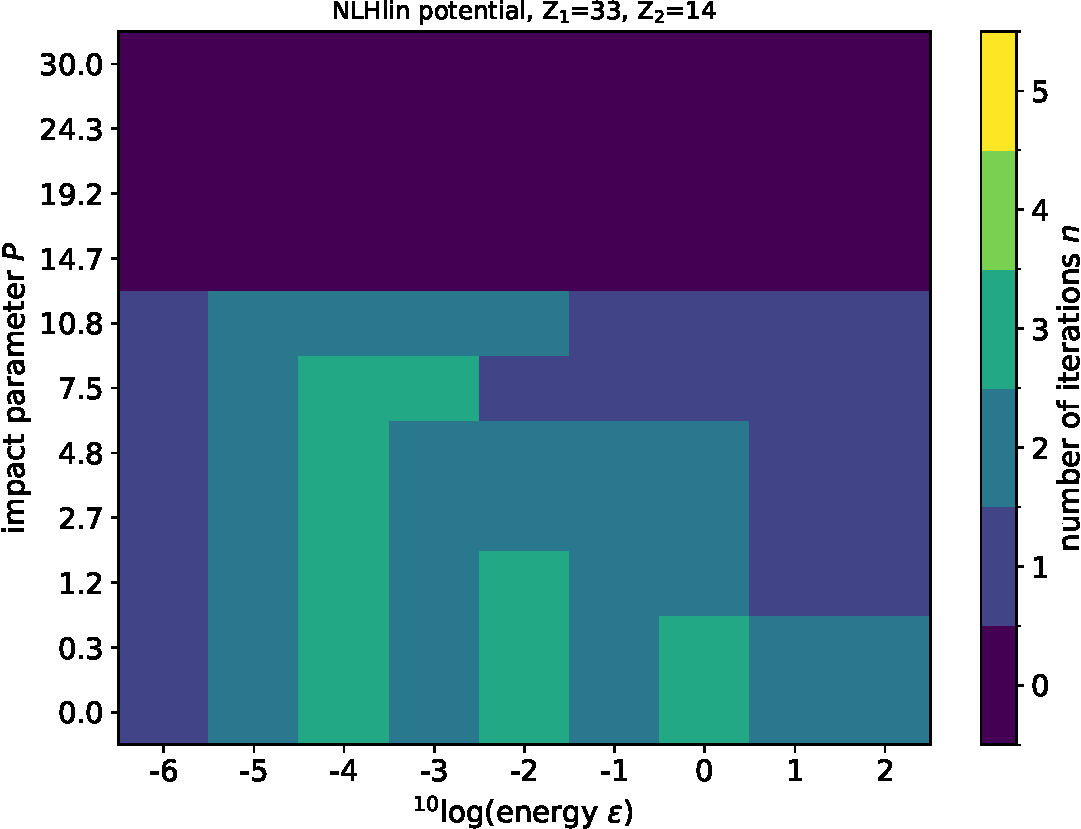
\includegraphics[scale=0.41]{NLHlin_iter_apsis_phiapprox.pdf}
    \caption{Number of iterations required to reach a relative accuracy of \(10^{-3}\) in \(R_0\) as a function of energy and impact parameter.
    Left: Universal ZBL potential.
    Right: NLHlin potential for As-Si using \cref{eq:sn_aNLH} as the screening length.
    The reduced impact parameters $P$ have been chosen as to cover the same range of unscaled impact parameters $p$.
    }
    \label{fig:iter-apsis_phiapprox}
\end{figure}
%
\Cref{fig:iter-apsis_phiapprox} shows the number of iterations required to reach a relative accuracy of \(10^{-3}\) between the last two calculated values of \(R_0\) for the universal ZBL and the NLHlin potential, using the approximations to $\Phi(R)$ described in this section for obtaining an initial condition.
Usually this means that the last value is accurate to \(10^{-6}\), assuming quadratic convergence has been reached.

From \cref{fig:iter-apsis_phiapprox} it is apparent that the NLHlin potential shows better convergence behavior than the ZBL potential at low projectile energies, while the convergence is similar for higher energies.


    \section{Variants of Newtons Method for Obtaining the Apsis of Collision (legacy)}
    \label{s:apsis_legacy}
    % Variants of Newtons Method for Obtaining the Apsis of Collision

\subsection{Iterating towards the Exact Solution}
%%%%%%%%%%%%%%%%%%%%%%%%%%%%%%%%%%%%%%%%%%%%%%%%%
\label{s:sn_apsis_iterating}
%
We consider three options for iteration:
%
\subsubsection{Newton’s method}
%
Newton's method to solve \cref{eq:sn_apsis_eq} for $R = R_0$ is given by \cref{eq:sn_apsis_newton}.
The initial condition \cref{eq:sn_apsis_ic} guarantees convergence of the iterations for screening functions with $\Phi'(R) < 0$ and $\Phi''(r) > 0$.

\subsubsection{Modified Newton's method}
%
Newton's method applied to \cref{eq:sn_apsis_eq} can also be interpreted as constructing the tangent lines to the terms $\Phi(R)/\varepsilon$ and $R - P^2/R$ and intersecting the two tangents, see the dashed lines in \cref{fig:apsis-iteration}.
%
\begin{figure}[htbp]
    \centering
    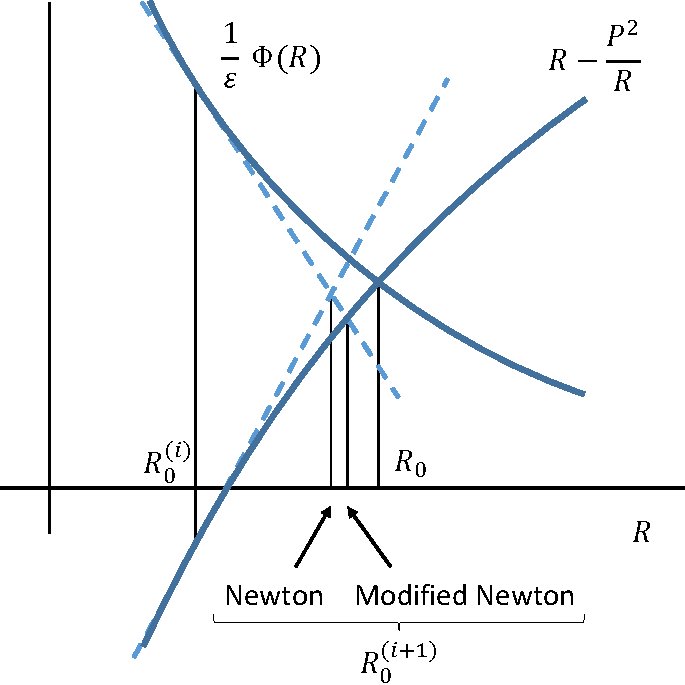
\includegraphics[scale=0.6]{apsis_iteration.pdf}
    \caption{Illustration of Newton’s method (linearization of both \(\Phi(R)\) and \(R-P^2/R\)) and the method based on linearization of \(\Phi(R)\) only.
    The latter comes closer to the actual solution \(R_0\).
    For both methods \(R_0^{(i)} < R_0^{(i+1)} < R_0\) provided \(R_0^{(i)} < R_0\).}
    \label{fig:apsis-iteration}
\end{figure}

Instead, one could also intersect the tangent to $\Phi(R)/\varepsilon$ with the function $R - P^2/R$.
The resulting quadratic equation has the solution%
%
\footnote{The other sign in front of the square root is not possible since all coefficients $a$, $b$, and $c$ are positive, which would result in a negative value of $R_0^{(i+1)}$.
}
%
\begin{equation}
    \label{eq:sn_apsis_linphi}
    R_0^{(i+1)} = \frac{ b + \sqrt{ b^2 + 4ac } }{ 2a }
\end{equation}
%
with
%
\begin{equation}
    \label{eq:sn_apsis_linphi_params}
    a = \varepsilon-\Phi'(R_0^{(i)}), \quad
    b = \Phi(R_0^{(i)}) - R_0^{(i)} \Phi'(R_0^{(i)}), \quad
    c = \varepsilon P^2
\end{equation}
%
As shown in \cref{fig:apsis-iteration}, both methods warrant \(R_0^{(i)} < R_0^{(i+1)} < R_0\) provided \(R_0^{(i)} < R_0\), as long as $\Phi''(R) > 0$.
In addition, \cref{fig:apsis-iteration} demonstrates that \cref{eq:sn_apsis_linphi} is a better approximation to \(R_0\) than \cref{eq:sn_apsis_newton}. This comes at the expense of another square root evaluation.

\subsubsection{Newton's method applied to $\log(f(R))$}
%
Instead of using \cref{eq:sn_apsis_newton} with \(f(R)\) from \cref{eq:sn_apsis_eq}, one can move the first and third term of $f(R)$  to the right-hand side of $f(R) = 0$, take the logarithm, and move the right-hand side back to the left-hand side.
One then obtains

\begin{equation}
    \label{eq:sn_apsis_newton_log}
    f_{\log}(R) = \log \left[ \frac{ 1 }{ \varepsilon } \Phi(R) \left/
        \left( R - \frac{ P^2 }{ R } \right)
        \right. \right]
        = 0
\end{equation}
%
The function \(f_{\log}(R)\) can be used with Newton’s method \cref{eq:sn_apsis_newton}.
It maintains the properties \(f_{\log}'(R) < 0\) and \(f_{\log}''(R) > 0\) for screening functions that are given by a sum of exponentials.
Therefore, Newton’s method is guaranteed to converge if one starts with an initial condition to the left of the solution.
The idea of taking the logarithm is to reduce the nonlinearity of \(f(R)\), but obviously comes at the expense of the evaluation of another special function.

\subsection{Convergence}
%%%%%%%%%%%%%%%%%%%%%%%%
\label{s:sn_apsis_performance}
%
\Cref{fig:iter-apsis-legacy} evaluates the perfomance of the combinations of initial condition and iteration algorithm for the ZBL screening function.
It shows the number of iterations required to reach a relative accuracy of \(10^{-3}\) between the last two calculated values of \(R_0\).
Usually this means that the last value is accurate to \(10^{-6}\), assuming quadratic convergence has been reached.

\begin{figure}[htbp]
    \centering
    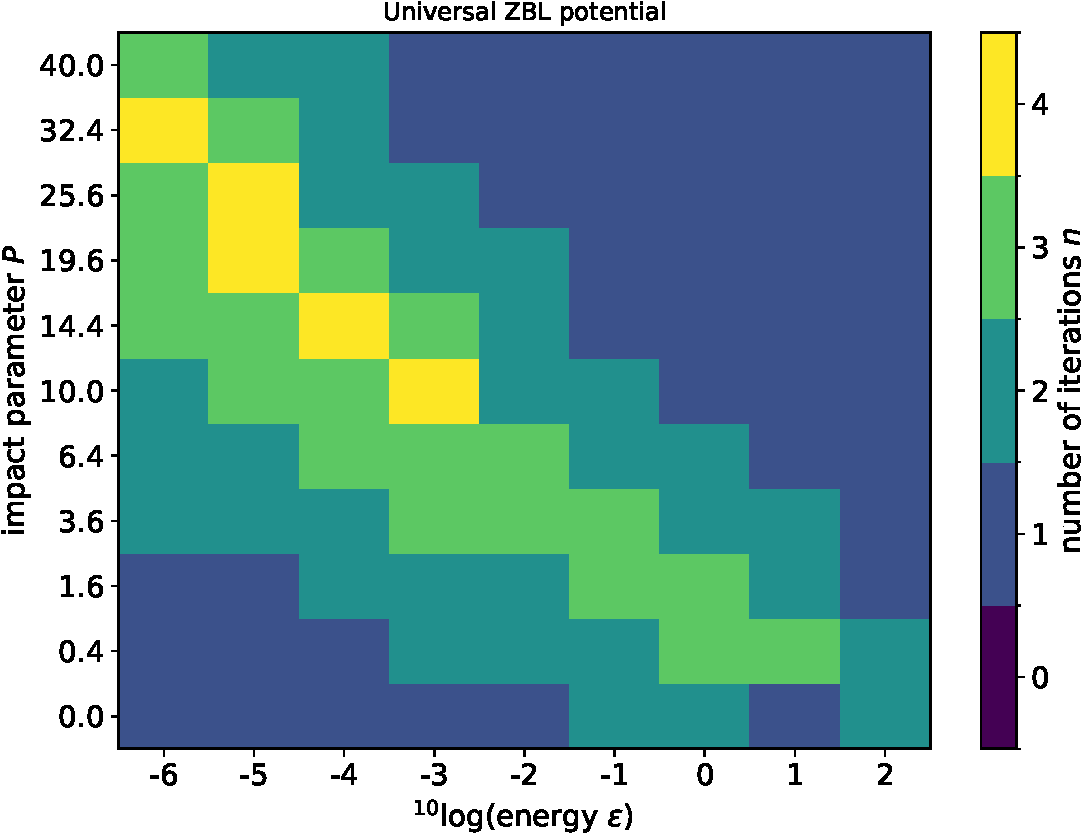
\includegraphics[scale=0.8]{iter_apsis_zbl.pdf}
    \caption{Number of iterations required to reach a relative accuracy of \(10^{-3}\) in \(R_0\) as a function of energy and impact parameter.
    Left column: using \(R_0^{(0)} = P\) \cref{eq:sn_apsis_ic_p} as initial condition.
    Right column: using \cref{eq:sn_apsis_ic} as initial condition.
    The columns differ by the iteration method used:
    First row: Newton.
    Second row: \cref{eq:sn_apsis_linphi} in the first iteration, then Newton.
    Third row: \cref{eq:sn_apsis_linphi} for all iterations.
    Fourth row: \cref{eq:sn_apsis_linphi} in the first iteration, then logarithmic Newton \cref{eq:sn_apsis_newton_log}.
    The interatomic potential used was the universal ZBL potential.}
    \label{fig:iter-apsis-legacy}
\end{figure}

In the left column, results for the initial condition \cref{eq:sn_apsis_ic_p} (\(R_0^{(0)} = P\)) are shown.
As expected, fewer iterations are required for large energies and large impact parameters (small deflection angles) than for small energies and small impact parameters (large deflection angles), since \(R_0\) is closer to \(P\).
For large deflection angles, more than 10 iterations may be required using ordinary Newton or \cref{eq:sn_apsis_linphi}.
Significant improvement is obtained by using the logarithmic function \cref{eq:sn_apsis_newton_log}, limiting the number of iterations to 6.
Note that Newton’s method with the logarithmic function cannot be started with \(R_0^{(0)} = P\), since this would lead to \(f_{\log}(R \rightarrow P) \rightarrow \infty\).
Therefore, \cref{eq:sn_apsis_linphi} has been used in the first iteration.

In the right column, the table of \(R_0^{(0,\varepsilon)}(\varepsilon)\) for head-on collisions has been used as described above.
Compared to the left column, the number of iterations at low energies and small impact parameters is significantly reduced (not couting the iterations necessary to obtain the table).
There are only slight differences in the iteration counts between the different iteration methods.
Using \cref{eq:sn_apsis_linphi} and \cref{eq:sn_apsis_newton_log} save one iteration in rare cases (compare first, second, and fourth row), while using \cref{eq:sn_apsis_linphi} beyond the first collision has no benefit (compare second and third row).
Since convergence is only marginally improved by using \cref{eq:sn_apsis_linphi} and \cref{eq:sn_apsis_newton_log}, while additional evaluations of a square root or a logarithm is necessary, using ordinary Newton’s method seems to be sufficient.

In summary, when no table of \(R_0^{(0,\varepsilon)}(\varepsilon)\) for head-on collisions is used, it is recommended to use \cref{eq:sn_apsis_linphi} in the first iteration and Newton’s method with the logarithmic function \cref{eq:sn_apsis_newton_log} for the remaining iterations. Significant acceleration is obtained by using the table of \(R_0^{(0,\varepsilon)}(\varepsilon)\) for head-on collisions to obtain an initial condition.
Then it is sufficient to use ordinary Newton’s method.
Note that the table needs to be calculated only once for a given interatomic potential.


    %\section{Scattering Angle in the CM System (legacy)}
    %\label{s:cmangle_legacy}
    %% Scattering Angle in the CM System
%
\subsubsection{Change of variables}
%%%%%%%%%%%%%%%%%%%%%%%%%%%%%%%%%%%
%
The integral in \cref{eq:sn_reduced_theta} is of the form
%
\begin{equation}
    \label{eq:sn_legacy_integration_integral_R}
    \int_{R_0}^\infty F(R) \, \mathrm{d}R .
\end{equation}
%
where \(R_0\) is a pole of $F(R)$, which is obtained by solving \cref{eq:sn_apsis}, see Section~\ref{s:apsis}.
Having a numerically determined pole of the integrand as an integration boundary is inconvenient, so the first step of calculating the scattering integrals is to apply a change of variable.
One possibility is \cite{Eck91}
%
\begin{equation}
    \label{eq:sn_legacy_transform1}
    R = \frac{ R_0 }{ (1-u^2) } .
\end{equation}
%
yielding
%
\begin{equation}
    \label{eq:sn_legacy_integration_integral_u1}
    \int_{R_0}^\infty F(R) \, \mathrm{d}R =
        2 R_0 \int_0^1 F \left( \frac{ R_0 }{ 1-u^2 } \right)
        \frac{ u \, \mathrm{d}u }{ (1-u^2)^2 } .
\end{equation}
%
With \cref{eq:sn_reduced_theta} we obtain
%
\begin{equation}
    \label{eq:sn_legacy_cmangl_legendre_theta_u}
    \theta = \pi - \frac{ 4 P }{ R_0 } \int_0^1
        \frac{ u \, \mathrm{d}u }{ g \left( \frac{ R_0 }{ 1-u^2 } \right) } .
\end{equation}
%
where $g(R)$ is given by \cref{eq:sn_reduced_g}.

\subsubsection{The integrand at the limits of integration}
%%%%%%%%%%%%%%%%%%%%%%%%%%%%%%%%%%%%%%%%%%%%%%%%%%%%%%%%%%
%
First, we show that the integrand is well-behaved.
For that, we write \(g(R_0/(1-u^2))\) explicitly
%
\begin{equation}
    \label{eq:sn_legacy_cmangl_legendre_g_u}
    g \left( \frac{ R_0 }{ 1-u^2 } \right) =
    \sqrt{ 1 - \frac{ 1 }{ \varepsilon R_0 }
        \Phi\left( \frac{ R_0 }{ 1-u^2 } \right) (1-u^2)
        - \frac{ P^2 }{ R_0^2 } (1-u^2)^2 } .
\end{equation}
%
By subtracting \cref{eq:sn_apsis} from the expression under the square root, \cref{eq:sn_legacy_cmangl_legendre_g_u} may be rewritten
%
\begin{equation}
    \label{eq:sn_legacy_cmangl_legendre_g_chi}
    g\left( \frac{ R_0 }{ 1-u^2 } \right) =
        \frac{ u }{ \sqrt{ \varepsilon R_0 } } \sqrt{ \chi(u) + \rho (2-u^2) }
\end{equation}
%
with
%
\begin{equation}
    \label{eq:sn_legacy_cmangl_legendre_chi}
    \chi(u) = \frac{ \Phi(R_0) - \Phi\left( \frac{ R_0 }{ 1-u^2 } \right) \, (1-u^2) }{ u^2 }
\end{equation}
%
and
%
\begin{equation}
    \label{eq:sn_legacy_cmangl_legendre_rho}
    \rho = \frac{ \varepsilon P^2 }{ R_0 } .
\end{equation}

\(\chi(u)\) is well-behaved with
%
\begin{equation}
    \label{eq:sn_legacy_cmangl_legendre_chi_lim}
    \chi(1) = \Phi(R_0), \qquad
        \lim_{u \rightarrow 0} \chi(u) = \Phi(R_0) - R_0 \Phi'(R_0) .
\end{equation}
%
The latter is obtained using l’Hospital’s rule.
\(\chi(u)\) is plotted in \cref{fig:sn-cmangl-legendre-chi-plot} for the universal ZBL potential and some values of \(R_0\).
%
\begin{figure}[htbp]
    \centering
    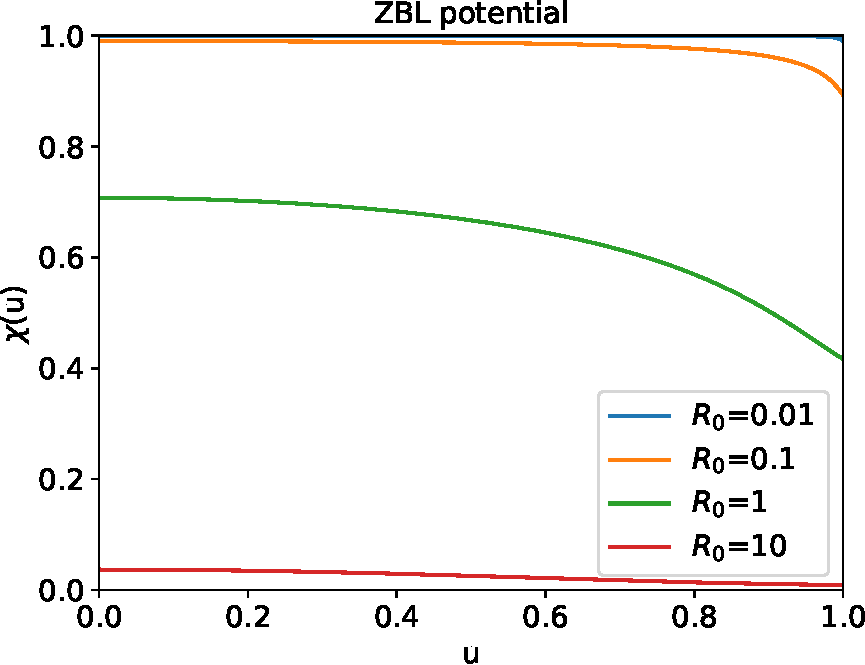
\includegraphics[scale=0.6]{chi_ZBL.pdf}
    \caption{Function \(\chi(u)\) according to \cref{eq:sn_legacy_cmangl_legendre_chi} for the ZBL universal potential.}
    \label{fig:sn-cmangl-legendre-chi-plot}
\end{figure}

\Cref{eq:sn_legacy_cmangl_legendre_theta_u} may now be rewritten
%
\begin{equation}
    \label{eq:sn_legacy_cmangl_legendre_theta_chi}
    \theta = \pi - 4 \int_0^1
    \sqrt{ \frac{ \rho }{ \rho \, (2-u^2) + \chi(u) } }
    \, \mathrm{d}u .
\end{equation}
%
Since \(\chi(u)\) is well-behaved, so is the term under the square root.
The integrand of \cref{eq:sn_legacy_cmangl_legendre_theta_chi} therefore has no poles, and the integral is amenable to standard methods of numerical quadrature.

\subsubsection{Integration using Gauss-Legendre quadrature}
%%%%%%%%%%%%%%%%%%%%%%%%%%%%%%%%%%%%%%%%%%%%%%%%%%%%%%%%%%%
%
Using Gauss-Legendre quadrature, we can approximate \cref{eq:sn_legacy_cmangl_legendre_theta_chi} by
%
\begin{equation}
    \label{eq:sn_legacy_cmangl_legendre_theta_chi_approx_plain}
    \theta \approx
        \pi - 4 \sum_{i=1}^n \tilde{w}_i
        \sqrt{ \frac{ \rho }{ \rho \, (2-\tilde{u}_i^2) + \chi(\tilde{u}_i) } }
\end{equation}
%
with \(\tilde{u}_i\) and \(\tilde{w}_i\) defined in \cref{eq:sn_legacy_legendre_transform} of Appendix~\ref{s:gauss-legendre}.

\Cref{eq:sn_legacy_cmangl_legendre_theta_chi_approx_plain}, however, has the problem that it does not tend to zero exactly as \(P \rightarrow \infty\).
Note that for \(\rho \rightarrow \infty\) the integral in \cref{eq:sn_legacy_cmangl_legendre_theta_chi} becomes
%
\begin{equation}
    \label{eq:sn_legacy_cmangl_legendre_pi}
    \int_0^1 \frac{ 1 }{ \sqrt{ 2-u^2 } } \, \mathrm{d}u = \frac{ \pi }{ 4 } ,
\end{equation}
%
and \(\theta \rightarrow 0\) as it should.
However, since the integrand is not a polynomial, the Legendre approximation of the integral will not evaluate exactly to \(\pi/4\), and \cref{eq:sn_legacy_cmangl_legendre_theta_chi_approx_plain} will not tend to zero as \(\rho \rightarrow \infty\).
This may be fixed by scaling the integral to the correct value of \(\pi/4\):
%
\begin{equation}
    \label{eq:sn_legacy_cmangl_legendre_theta_chi_approx}
    \theta \approx
        \pi \left( 1
        - \frac{ 4 }{ \pi_\mathrm{num} }
        \sum_{i=1}^n \tilde{w}_i \sqrt{
            \frac{ \rho
            }{ \rho \, (2-\tilde{u}_i^2) + \chi(\tilde{u}_i) } }
        \right)
\end{equation}
%
with
%
\begin{equation}
    \label{eq:sn_legacy_cmangl_legendre_pinum}
    \pi_\mathrm{num} =
        4 \sum_{i=1}^n \tilde{w}_i \frac{ 1 }{ \sqrt{ (2-\tilde{u}_i^2) } }
\end{equation}
%
Since the sum in \cref{eq:sn_legacy_cmangl_legendre_theta_chi_approx} evaluates to \(\pi_\mathrm{num}/4\) for \(\rho \rightarrow \infty\), \(\theta \rightarrow 0\).
At the same time, for \(\rho \rightarrow 0\) (i.e., \(P \rightarrow 0\)) the sum goes to zero and \(\theta \rightarrow \pi\) as it should.

One can also apply this correction to the Legendre approximation of \cref{eq:sn_legacy_cmangl_legendre_theta_u}:
%
\begin{equation}
    \label{eq:sn_legacy_cmangl_legendre_theta_g_approx}
    \theta \approx
        \pi \left( 1 - \frac{ 4 }{ \pi_\mathrm{num} } \frac{ P }{ R_0 }
        \sum_{i=1}^n
        \frac{ \tilde{w}_i \tilde{u}_i
        }{ g \left( \frac{ R_0 }{ 1-\tilde{u}_i^2 } \right) } \right).
\end{equation}
%
\Cref{eq:sn_legacy_cmangl_legendre_theta_g_approx} is not numerically equivalent to \cref{eq:sn_legacy_cmangl_legendre_theta_chi_approx}.
It does not require the evaluation of \(\Phi(R_0)\), which might represent a non-negligible saving of computation time if few abscissas are used.
For few abscissas, the results of \cref{eq:sn_legacy_cmangl_legendre_theta_g_approx} and \cref{eq:sn_legacy_cmangl_legendre_theta_chi_approx} are very similar.
With increasing number of abscissas, the result is increasingly dependent on the accuracy of the apsis \(R_0\).
The term under the square root may even become negative, if the accuracy of \(R_0\) is low and the number of abscissas is large.

The integrand of \cref{eq:sn_legacy_cmangl_legendre_theta_chi} is shown in \cref{fig:integrand-legendre-theta} for the limiting cases \(\rho \gg \Phi, \chi\) and \(\rho \ll \Phi, \chi\).
It is smooth, although not completely polynomial (note the long flat parts of most curves).%
%
\footnote{Alternatively, one may insert \cref{eq:sn_legacy_cmangl_legendre_pinum} in \cref{eq:sn_legacy_cmangl_legendre_theta_chi_approx_plain} instead of \(\pi\), and one gets after some manipulation and correction with \(\pi / \pi_\mathrm{num}\)
%
\begin{equation*}
    \theta \approx 4 \frac{ \pi }{ \pi_\mathrm{num} } \sum_{i=1}^n
        \tilde{w}_i
        \frac{ \chi(\tilde{u}_i)
        }{ \sqrt{ 2-\tilde{u}_i^2 } \,
            ( S_1(\tilde{u}_i) + S_2(\tilde{u}_i) ) \,
            S_2(\tilde{u}_i) } .
\end{equation*}
%
with
%
\begin{equation*}
    S_1(u) = \sqrt{ \rho \, (2-u^2) }, \qquad
    S_2(u) = \sqrt{ \rho \, (2-u^2) + \chi(u) } .
\end{equation*}
%
This also guarantees \(\theta \rightarrow 0\) as \(\rho \rightarrow \infty\), and due to the correction also \(\theta \rightarrow \pi\) as \(\rho \rightarrow 0\).
While this has, in principle, better roundoff behavior, the improvement is insignificant for the small numbers of abscissas investigated here.}
%
\begin{figure}[htbp]
    \centering
    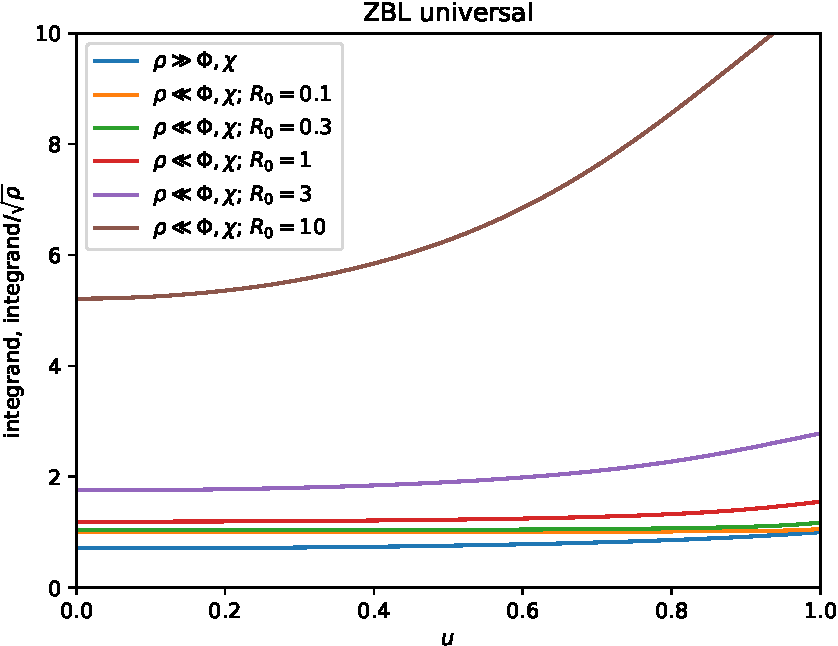
\includegraphics[scale=0.6]{integrand_legendre_theta.pdf}
    \caption{Integrand of \cref{eq:sn_legacy_cmangl_legendre_theta_chi} for \(\rho \gg \Phi, \chi\) and \(\rho \ll \Phi, \chi\).
    For \(\rho \gg \Phi, \chi\) the function is independent of \(R_0\).
    For \(\rho \ll \Phi, \chi\) the integrand divided by \(\sqrt{\rho}\) is plotted for some \(R_0\) values.}
    \label{fig:integrand-legendre-theta}
\end{figure}

\subsubsection{Convergence}
%%%%%%%%%%%%%%%%%%%%%%%%%%%
%
In \cref{fig:error-legendre-theta-1e-6}, the relative errors in \(\theta\) as calculated by \cref{eq:sn_legacy_cmangl_legendre_theta_chi_approx_plain}, \cref{eq:sn_legacy_cmangl_legendre_theta_chi_approx}, and \cref{eq:sn_legacy_cmangl_legendre_theta_g_approx} are shown as a function of impact parameter for \(\varepsilon = 10^{-4}\), \(\varepsilon = 10^{-1}\), and \(\varepsilon = 100\).
The curves obtained from \cref{eq:sn_legacy_cmangl_legendre_theta_chi_approx} (solid lines) and \cref{eq:sn_legacy_cmangl_legendre_theta_g_approx} (dotted lines) are indistinguishable.
The lines corresponding to \cref{eq:sn_legacy_cmangl_legendre_theta_chi_approx_plain} (dashed lines) show significantly larger errors for small numbers of abscissas and large impact parameters (small scattering angles), demonstrating the significance of the scaling with the numerical value of \(\pi\).
%
\begin{figure}[htbp]
    \centering
    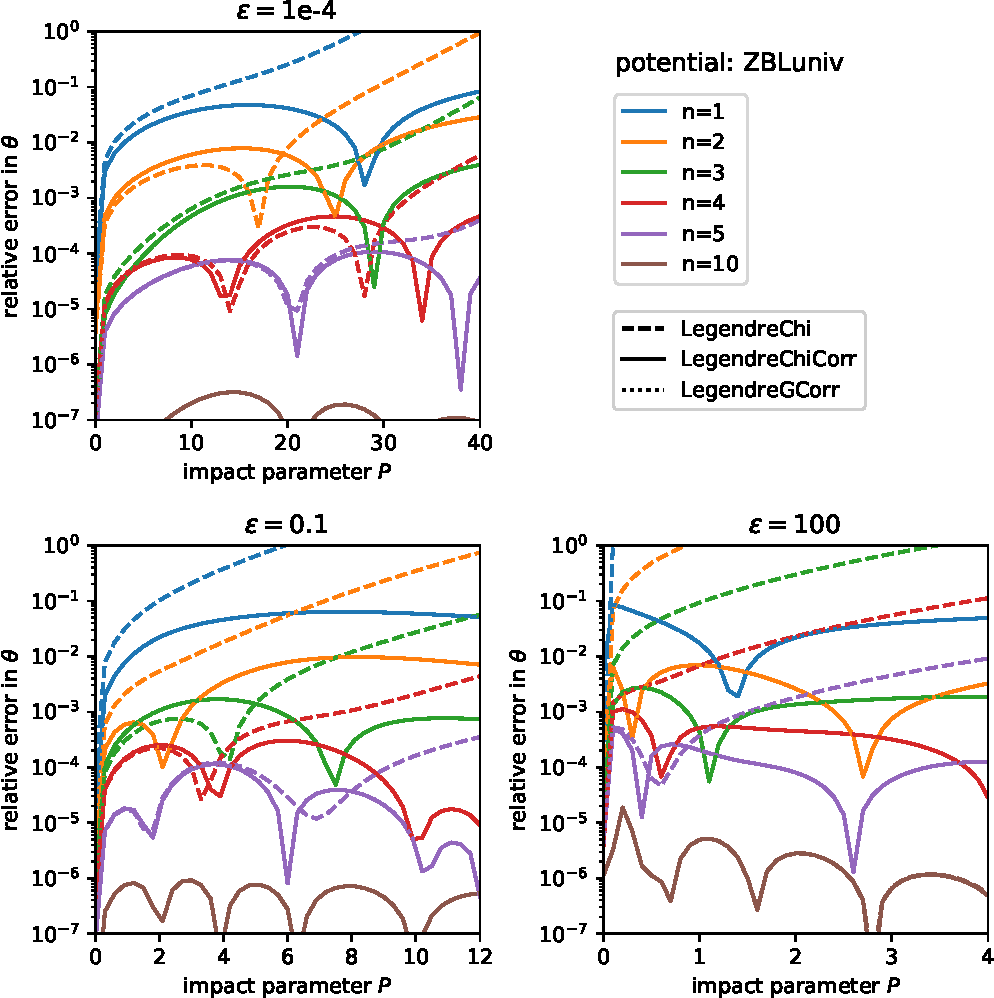
\includegraphics[scale=0.6]{error_legendre_theta_1e-6.pdf}
    \caption{Relative errors in \(\theta\) of n-point Gauss-Legendre quadrature as a function of reduced impact parameter for three energies.
    Dashed lines: \cref{eq:sn_legacy_cmangl_legendre_theta_chi_approx_plain},
    solid lines: \cref{eq:sn_legacy_cmangl_legendre_theta_chi_approx},
    dotted lines: \cref{eq:sn_legacy_cmangl_legendre_theta_g_approx}.
    The reference simulation evaluated \cref{eq:sn_legacy_cmangl_legendre_theta_chi_approx} with 100-point Gauss-Legendre quadrature.
    The relative accuracy of the apsis is better than \(10^{-6}\).}
    \label{fig:sn_legacy_error-legendre-theta-1e-6}
\end{figure}

In \cref{fig:error-legendre-theta-1e-6}, a relative accuracy of \(10^{-6}\) was imposed on the apsis \(R_0\).
In \cref{fig:error-legendre-theta-1e-3}, the same results for the relative error are shown for a relative accuracy of \(10^{-3}\).
Now the results for \cref{eq:sn_legacy_cmangl_legendre_theta_g_approx} clearly deteriorate.
So, the saving of the evaluation of \(\Phi(R_0)\) in calculating \cref{eq:sn_legacy_cmangl_legendre_theta_g_approx} is approximately compensated for by another iteration required for obtaining \(R_0\).
Considering the risk of producing negative arguments of the square root in \cref{eq:sn_legacy_cmangl_legendre_theta_g_approx}, \cref{eq:sn_legacy_cmangl_legendre_theta_chi_approx} seems preferable.
%
\begin{figure}[htbp]
    \centering
    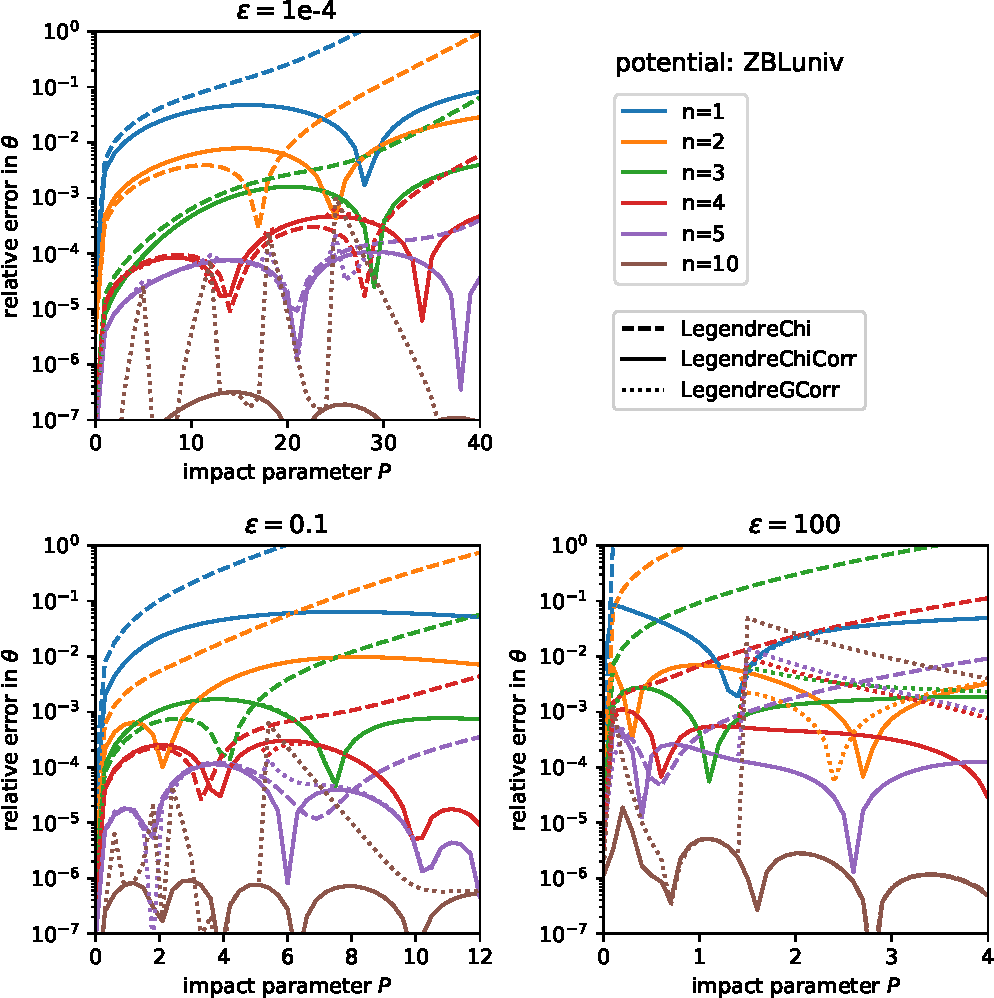
\includegraphics[scale=0.6]{error_legendre_theta_1e-3.pdf}
    \caption{Relative errors in \(\theta\) of n-point Gauss-Legendre quadrature as a function of reduced impact parameter for three energies.
    Dashed lines: \cref{eq:sn_legacy_cmangl_legendre_theta_chi_approx_plain},
    solid lines: \cref{eq:sn_legacy_cmangl_legendre_theta_chi_approx},
    dotted lines: \cref{eq:sn_legacy_cmangl_legendre_theta_g_approx}.
    The reference simulation evaluated \cref{eq:sn_legacy_cmangl_legendre_theta_chi_approx} with 100-point Gauss-Legendre quadrature.
    The relative accuracy of the apsis is better than  \(10^{-3}\).}
    \label{fig:sn_legacy_error-legendre-theta-1e-3}
\end{figure}

\end{subappendices}
%
%%%%%%%%%%%%%%
% Literature %
%%%%%%%%%%%%%%
%
\bibliography{nuclear_scattering}
%
\end{document}
